% !TEX root = ../thesis.tex
\graphicspath{{Chapter2/Chapter2Figs/}{Chapter2/Chapter2Figs/}}
 
% \chapter{Use a Fine-Tuned Large Language Model to Generate Consistent and Sufficient Synthetic Texts}\label{ch:chapter:2}
\chapter{Synthetic Texts Generation with a Fine-tuned Large Language Model}\label{ch:chapter:2}



\begin{Abstract}
This study proposes a framework for generating structured synthetic policy communication by post-training a large language model (LLM) on Federal Open Market Committee (FOMC) materials and macro-financial indicators. We first adapt a reasoning-capable backbone to produce domain-consistent economic and financial analysis, and then align selected outputs with the institutional tone and section structure of official FOMC Minutes. Empirically, we evaluate the resulting checkpoints along four dimensions: (i) textual fidelity to reference sections, (ii) input grounding under leave-one-out masking, (iii) exploratory sentiment--return regressions, and (iv) decision prediction benchmarked against historical, econometric, and market-implied baselines where data coverage permits. The Chapter 2 v2 pipeline is organized around meeting-level fixed random 80/10/10 splits, so the reported evidence should be interpreted as held-out meeting validation rather than as a chronological forecasting design.
\end{Abstract}


\section{Introduction}\label{ch2:sec:introduction}


Government announcements materially influence interest-rate markets (\cite{vergote2012}; \cite{rosa2013financial}; \cite{jubinski2013fomc}). Among these, the Federal Open Market Committee (FOMC) plays a particularly critical role in shaping both the U.S. and global economic outlook through its monetary policy decisions—most notably, adjustments to the target range of the federal funds rate, which have direct and immediate effects on the government bond market. Moreover, U.S. government bond derivatives, such as the 10-Year Treasury Note futures and options, are traded nearly continuously, with only a one-hour pause from 4 p.m. to 5 p.m. Central Time (CT). This trading structure permits high-frequency studies of market responses to policy communication. The empirical diagnostic in this chapter, however, uses release-day closes and does not isolate an instantaneous intraday response.


A related text-as-data literature documents associations between textual
sentiment and financial outcomes (\cite{bollen2011twitter}; \cite{ding2015deep}; \cite{ding2016knowledge}; \cite{xu2018stock}). Such associations do not establish that sentiment is a single causal driver of market movements. Central-bank communication is multidimensional, and a document can convey policy-path or economic-information news that a scalar tone score does not recover.


Policy meetings and institutional documents also form a sparse historical record, motivating controlled synthetic-data exercises. 


However, unlike quantitative data, these qualitative data are inherently discontinuous, making historical data insufficient for analyzing a wide range of potential scenarios. For instance, the Federal Reserve has adjusted the federal funds rate only 130 times since the 1990s. To address this challenge, we propose leveraging a fine-tuned large language model (LLM) to generate synthetic texts across a variety of scenarios, thereby enhancing the capability of volatility models to incorporate qualitative inputs.



On the other hand, recent advances in neural networks and LLMs have led to remarkable performance improvements across a broad range of natural language processing (NLP) tasks. LLMs are pre-trained on vast and diverse text corpora, which can be adapted to domain-specific tasks and have already been used for synthetic data generation in multiple settings (\cite{schick2021generating}; \cite{peng2023instruction}; \cite{yu2024large}; \cite{li2021synthetic}; \cite{meoni2024generating}). In finance, synthetic datasets are also used for robustness testing (\cite{cao2022synthetic}; \cite{carvajal2022synthetic}).



Moreover, synthetic data have been widely accepted by financial researchers as powerful tools for robustness testing. For instance, \cite{cao2022synthetic} created a synthetic limit order book to evaluate forecasting models, while \cite{carvajal2022synthetic} used synthetic stock prices to train trading algorithms. Beyond time-series data, the financial industry manages vast volumes of structured documents, such as financial reports, Bank of England Monetary Policy Committee (MPC) meeting minutes, and Federal Reserve FOMC meeting minutes. The simulation capabilities of LLMs make them ideal for generating synthetic structured textual data in these contexts.


This chapter studies a shared-parent, two-branch post-training design on LLM. First, \textit{Model chk-1} maps point-in-time macro-financial evidence into analytical narratives and provides the common analytical representation. From this parent, \textit{Model chk-2} is trained to rewrite a supplied analysis as source-preserving FOMC-Minutes-style prose, whereas \textit{Model chk-3} is trained separately to map a target-neutral pre-meeting analysis into a monetary-policy action.

After that, we then evaluate whether the synthetic text is stylistically faithful, input-grounded, and economically meaningful through prompt-contribution tests, sentiment-return regressions, and policy-decision prediction.



\subsection*{Research Motivation}

The motivation for this research arises from the critical importance of accurately forecasting monetary policy decisions and the well-recognized limitations of traditional econometric models in capturing qualitative and contextual signals. Firstly, monetary-policy forecasting remains important for asset pricing and risk management. Secondly, conventional quantitative models do not fully exploit textual policy signals from minutes, statements, and staff discussions. As a result, they may miss informative cues about policy direction.


LLMs provide a practical route to close this gap by integrating structured
indicators with unstructured text. Furthermore, evidence on using LLMs to simulate committee-style policy communication and decision-relevant reasoning is still limited. Hence, this chapter addresses that gap through a scenario-based simulation framework. More specifically, the framework is designed to (i) generate Minutes-style synthetic texts under alternative macro-financial conditions and (ii) evaluate whether such synthetic communications preserve policy-relevant signals, including the ability to infer the direction of policy-rate changes



\subsection*{Research Questions}

This chapter investigates whether large language models can be used as simulation tools for monetary-policy communication and decision support. The main research question is:

\textit{Can a fine-tuned, reasoning-capable LLM generate FOMC-Minutes-style sections grounded in macroeconomic and financial indicators, and do those synthetic texts preserve policy-relevant signals such as market impact and policy-rate outcomes?}

To address this central question, we study the following sub-questions:

\begin{itemize}
\item[1.] To what extent can a fine-tuned LLM reason over macro-financial indicators and extract policy-relevant insights?

\item[2.] Can the framework replicate the structured deliberation and trade-off language observed in FOMC discussions?

\item[3.] How closely do generated sections match the tone, format, and information content of authentic Minutes?

\item[4.] How does model-based decision prediction on historical FOMC actions?
\end{itemize}

These questions concern observable output fidelity, semantic alignment,
prompt sensitivity, classifier-score closeness, historical association,
policy-action accuracy, and delivery. 



\subsection*{Contribution}

This study makes several important contributions to the literature at the intersection of central banking, financial economics, and artificial intelligence:

\begin{itemize}
\item[] \textbf{Shared-Parent, Two-Branch Design:} We develop a common analytical model followed by two independently evaluated downstream branches: analysis-to-FOMC-Minutes-style paragraph rewriting and analysis-to-policy-action prediction. The decision branch is a separate post-training comparison.

\item[] \textbf{Extension of LLM Applications:} This study applies
domain-specific LLM post-training to controlled institutional-text rewriting and policy-action diagnostics, extending its use beyond conventional text classification and information retrieval.


\item[] \textbf{Minutes-Style Text Rewriting:} We compare raw-best-effort semantic similarity to synthetic teacher references across the base, analytical-SFT, and Minutes-SFT checkpoints on 391 released samples from 124 meetings. This is a training-release reconstruction diagnostic; similarity scores alone do not establish numerical fidelity, source preservation, or held-out generalization.


\item[] \textbf{Independent Decision-Branch Diagnostic:} We compare decision SFT with its post-GRPO descendant under a common action and response contract, reporting policy-action quality, native structured delivery, and the engineered proxy score separately.


\item[] \textbf{Multi-Dimensional Evaluation:} We evaluate synthetic Minutes not only with text-based similarity metrics, but also with grounding (prompt-contribution) tests and economics-based validations (market relevance and decision prediction), thereby providing a more comprehensive notion of ``realism'' than surface-level textual resemblance alone.
\end{itemize}


Finally, our findings offer actionable insights for central banks, financial market participants, and policymakers by demonstrating the potential of LLMs to augment human decision-making under conditions of uncertainty and information overload.




\subsection*{Chapter Structure}

This chapter is organized as follows. Section~\ref{ch2:sec:lr} reviews the related literature on synthetic data and large language models. Section~\ref{ch2:sec:2-step-training} outlines the shared-parent, two-branch post-training design. Section~\ref{ch2:sec:the-dataset} describes the dataset construction process and prompt templates. Section~\ref{ch2:sec:base_model} introduces the base model, while Sections~\ref{ch2:sec:training} and~\ref{ch2:sec:parameter} describe the fine-tuning method and hyperparameter settings. Section~\ref{ch2:sec:application} presents the evaluation dimensions and empirical tests, and Section~\ref{ch2:sec:result} reports the training and evaluation results. Finally, Section~\ref{ch2:sec:conclusion} concludes the chapter and discusses future research.



\section{Literature Review}\label{ch2:sec:lr}

\subsection*{Related Works on Synthetic Data}\label{ch2:sec:lr:related work}
Current literature on synthetic data generation has shown remarkable improvement with the significant advancement of the Generative Artificial Intelligence (AI) technologies. 


The Royal Society (\cite{jordon2022synthetic}) defines synthetic data as \textit{``... data that has been generated using a purpose-built mathematical model or algorithm, with the aim of solving a (set of) data science task(s)''}. Traditional approaches to generating synthetic data focus on quantitative data and rely on numerical procedures based on specific assumptions and random numbers drawn from distributions such as the normal or uniform distribution. Examples include the Autoregressive Moving Average model (ARMA; \cite{whittle1951hypothesis}) and the Generalized Autoregressive Conditional Heteroskedasticity model (GARCH; \cite{Bollerslev:1986}). However, recent advances in Artificial Neural Networks (ANNs) and Large Language Models (LLMs) have introduced new approaches to generating not only numerical data but also textual data. LLMs, which are pre-trained on a wide range of existing textual data, can successfully capture various linguistic features and generate human-like text.



Prior surveys (\citet{potluru2023synthetic}; \citet{assefa2020generating}; \citet{guo2024generative}) summarize LLM-based synthetic text generation and emphasize three persistent issues: controllability, privacy, and evaluation. In macro-finance, the small number of major policy episodes further motivates simulation-based methods in which text is generated conditionally on counterfactual indicator paths.


A parallel literature studies the informational content of FOMC communications using text mining and sentiment methods. \citet{huang2021economic} show predictive value in FOMC text, and event-study evidence finds market effects around Minutes releases (\cite{jubinski2013fomc}; \cite{tadle2022fomc}). Emerging studies on generative AI for policy analysis provide additional motivation for Minutes-style synthetic generation and for evaluation designs that test economic relevance rather than style alone (\cite{dunn2024using}).

\subsection*{Large Language Models (LLMs) for Structured Text Generation}\label{ch2:sec:lr:llm}


Transformer-based LLMs are the dominant architecture for text generation and representation learning. Chapter~\ref{ch:ch0} (Section~\ref{sec:ch0:ml-finance}) reviews Transformer foundations, GPT/BERT model families, and fine-tuning strategies. In this chapter, we treat the LLM as a conditional generator: given prompts that encode macro-financial indicators and policy context, the model generates section-level policy narratives. This maps naturally to scenario analysis, where each indicator path corresponds to one scenario and the generated Minutes-style text acts as a document-level representation of that scenario.


\subsection*{Consistent Texts}\label{ch2:sec:lr:text}


LLMs can generate human-like text, but ensuring \textit{consistency} remains challenging, especially for long-form and structured documents. In this chapter, consistency has two dimensions: (i) internal coherence across paragraphs and sections, and (ii) faithfulness to conditioning inputs (macroeconomic and financial indicators). A common failure mode is hallucination, where generated claims are unsupported by inputs or conflict with external facts (\cite{huang2025survey}).

Because base LLMs are optimized for broad-domain and general-purpose text, their default behavior may not match the style constraints and evidence standards required in specialized domains. Fine-tuning addresses this mismatch by aligning the model with task-specific constraints. For instance, the Llama family has been fine-tuned into variants optimized for different use cases, such as dialogue-oriented chat models and code-focused models (\cite{llama-recips}). In our setting, fine-tuning is used to align the model with (i) macro-financial reasoning grounded in numerical indicators and (ii) the formal, section-structured writing conventions of FOMC Minutes, thereby reducing inconsistency and unsupported generation.

These considerations motivate both the sequential supervised fine-tuning framework in Section~\ref{ch2:sec:training-plan} and the evaluation design in Section~\ref{ch2:sec:application}.




\section{2-Step Training Plan}\label{ch2:sec:2-step-training}

To develop a model that can (i) conduct macro-financial analysis from structured indicators and (ii) support downstream FOMC-style generation and policy-simulation tasks, we separate the workflow into one \textit{core} two-step post-training pipeline and two \textit{task-specific} downstream adaptations. The core pipeline consists of Supervised Fine-Tuning (SFT) followed by Reinforcement Learning (RL) using Group Relative Policy Optimization (GRPO). The downstream adaptations then specialize the analysis checkpoint for either Minutes-style rewriting or decision prediction.

In Step 1 (SFT), we adapt the backbone model to map macroeconomic and financial indicators into structured analytical outputs. SFT provides a stable reference-guided objective and establishes the domain-specific analysis style used throughout the rest of the chapter.

In Step 2 (GRPO), we refine reasoning quality with task-specific rewards. In the reported analysis run, the reward signal is derived from answer-level analytical quality and reasoning consistency rather than token-level supervised references. This step is intended to reduce unsupported generation and improve the logical consistency of the analytical response.

The key modeling point is that not every empirical table in this chapter uses the same checkpoint. The reported experiments draw from four archived checkpoints, summarized in Table~\ref{tab:ch2:checkpoint_map}. This mapping closes the model lineage that would otherwise remain ambiguous if ``baseline model'', ``fine-tuned model'', and ``Minutes-aligned model'' were used interchangeably.

\begin{table}[htbp]
    \centering
    \footnotesize
    \begin{tabular}{p{0.17\textwidth} p{0.18\textwidth} p{0.25\textwidth} p{0.3\textwidth}}
        \toprule
        \textbf{Checkpoint} & \textbf{Parent} & \textbf{Primary Role} & \textbf{Archived Evidence in Repository} \\
        \midrule
        Backbone-0 & --- & Reasoning-capable experimental backbone & \texttt{models/DeepSeek-R1-Distill-Llama-8B} \\
        Checkpoint-1 & Backbone-0 & Analysis SFT checkpoint for domain adaptation & \texttt{output/training/main/merged/analysis\_sft} \\
        Checkpoint-2 & Checkpoint-1 & Analysis GRPO checkpoint for reward-refined reasoning & \texttt{output/training/main/merged/analysis\_grpo} \\
        Checkpoint-3 & Checkpoint-1 & Minutes-style alignment checkpoint for rewriting analytical summaries into official FOMC style & \texttt{output/training/main/merged/minutes\_alignment\_sft} \\
        Checkpoint-4 & Checkpoint-1 & Decision-specific GRPO checkpoint for policy-action prediction & \texttt{output/training/main/merged/decision\_grpo} \\
        \bottomrule
    \end{tabular}
    \caption{Checkpoint Mapping for the Reported Chapter 2 Experiments}
    \label{tab:ch2:checkpoint_map}
\end{table}

Table~\ref{tab:ch2:checkpoint_map} also clarifies an important scope boundary. Checkpoint-3 is used only for Minutes-style rewriting tasks, while Checkpoint-4 is a separate decision-specific branch. Consequently, a result reported for Checkpoint-3 should not be interpreted as evidence about Checkpoint-4, and vice versa.

Overall, the two-step analysis pipeline (Checkpoint-1 and Checkpoint-2) should be interpreted as the common analytical foundation. The Minutes-style generation task and the decision-prediction task then build separate downstream branches on top of that foundation. This separation is essential for interpreting the empirical results with the correct attribution.




\newcommand{\inputtag}[1]{**\textless #1\textgreater**}



\section{Dataset Construction}\label{ch2:sec:the-dataset}

This section describes the construction of the training corpus. The raw text comes from Federal Open Market Committee (FOMC) Minutes and is paired with macroeconomic and financial indicators. We then process these sources into structured samples for model training and evaluation.


\subsection*{FOMC Minutes and Indicators}\label{ch2:sec:raw_data}


The Federal Open Market Committee (FOMC) meetings have been recorded since the committee's formation under the Banking Act of 1935 (\cite{todd2016corollary}). Initially, from 1936 to 1967, the minutes were released only once a year in these early years. Between 1967 and 1992, the minutes were named as ``the Minutes of Actions''. combined with ``the Record of Policy Actions'', these documents provided detailed insights not only into the policies but also the reasoning and proceedings behind them. Starting in 1993, a timely record of all policy issues and decisions made by the Committee was published after each meeting, although the documentation lacked a structured format. After 2009, the minutes were organized into distinct sections, including "Economic Situation," "Financial Situation," "Economic Outlook," and "Committee Policy Action," and the Committee has continued to use this structure to the present day. 

Because early records were less frequent and less standardized, while post-2009 Minutes adopted a relatively stable section structure and section-level consistency is essential for supervised alignment, we use post-2009 Minutes as the primary source corpus.




We downloaded Minutes from January 2009 to January 2025 from the Federal Reserve website as the \textbf{main text corpus}. Given the stable section structure after 2009, we parsed major sections ( ``Staff Review of the Economic Situation'', ``Staff Review of the Financial Situation'', ``Staff Economic Outlook'', ``Participants' Views on Current Conditions and Economic Outlook'', and ``Committee Policy Actions'') when available, yielding 486 section-level samples. We also collected Minutes from February 1993 to December 2008 as a \textbf{supplementary corpus}. Because these earlier files lack stable section headings, they require additional processing described below.

Table~\ref{tab:ch2:summary_statis} reports token-level summary statistics for both full Minutes and extracted sections under the tokenizer used in our experiments. Across the sample, Minutes length ranges from roughly 8,000 to 25,000 tokens, while most individual analytical sections fall below 4,096 tokens.


In this chapter, ``word'' does not necessarily mean a full lexical word. LLMs operate on tokens (often sub-word units). For example, ``Negative'' may be split into smaller units such as ``Neg'' and ``ative''. This tokenization is controlled by the model-specific tokenizer. Larger models often use larger vocabularies; for example, GPT-4 class models use larger token vocabularies, while LLaMA 3 uses a 128,000-token vocabulary. Table~\ref{tab:ch2:summary_statis} reports token-level summary statistics.


\begin{table}[htbp]
    \scriptsize
    \centering
    \begin{tabular}{p{3.8cm}cccccccc}
        \toprule
        Names&                                                Count&	    Mean&	    Std&	 Min&	   25\%&	  50\%&	   75\%&	Max \\
        \hline
        Total Minutes&	                                        123&	15119.50&	5136.89&	8144&	  10545&	 13117&	  20234&	25106 \\
        Total Sections&	                                        486&	 2883.71&	2921.00&	 294&	 1391.5&	1729.5&	3014.75&	13621\\
        Staff Economic Outlook&	                                123&	 3002.20&	 779.20&	 294&	   2556&	  3076&	   3481&	5080 \\
        Staff Review of the Economic Situation&	                120&	 1348.81&	 314.13&	 653&	1178.25&	  1356&	   1490&	2929 \\
        Staff Review of the Financial Situation&	            119&	 1491.61&	 291.48&	 903&	   1293&	  1479&	 1643.5&	2461 \\
        Committee Policy Action&	                            122&	 5625.28&	4646.81&	1262&	   1770&	2448.5&	  11118&	13621 \\
        Staff Review of the Economic and Financial Situation&	  2&	    3286&	 200.82&	3144&	   3215&	  3286&	   3357&	3428 \\
        \bottomrule
    \end{tabular}
    \caption{Summary Statistics for Tokens of Different Sections and Minutes}
    \label{tab:ch2:summary_statis}
\end{table}


Because most major sections are shorter than 4,096 tokens (except ``Committee Policy Action''), we cap the assistant output length at 4,096 tokens to control memory usage.




\subsection*{From FOMC Minutes to Analysis}


Because our prompts are constructed from macroeconomic and financial indicators, we must map unstructured Minutes paragraphs to the corresponding indicator topics. We use an LLM (ChatGPT-4o) as a \textit{weakly supervised classifier} to assign indicator labels to Minutes paragraphs, which enables systematic alignment between numerical inputs and textual targets. Since LLM-based labeling can introduce noise or bias, we mitigate this risk by (i) manually cleaning and standardizing the label ontology and (ii) relabeling with a constrained reference list after cleaning. Importantly, we exclude administrative paragraphs and the ``Committee Policy Action'' content from the \textit{analysis-generation} dataset to avoid leaking realized policy decisions into training, which is crucial for a fair decision-prediction evaluation later in the chapter.


To construct candidate indicator labels, we first asked the LLM to label paragraphs without a predefined reference list. These model-generated tags are treated as \textit{raw labels}. We then identified several quality issues that required cleaning and standardization.

First, some of the raw labels were too general or lacked measurable indicators—for example, labels like ``Housing'', ``International Markets'', ``Swap Arrangements'', and ``Liquidity Facilities''. These categories do not correspond to specific economic indicators.

Second, different labels were often used for the same underlying indicator. For instance, ``PCE Price Index'', ``Consumer Spending'', and ``Personal Consumption Expenditures (PCE)'' all refer to the same economic concept and were consolidated under ``Personal Consumption Expenditures (PCE)''.


Finally, some labels represented subcomponents of broader constructs. For example, ``Total Assets of the Federal Reserve'' and ``Total Liabilities of the Federal Reserve'' were consolidated under ``Federal Reserve Balance Sheet''.


Therefore, we manually cleaned the \textit{raw labels} and created a list of \textit{reference labels} based on them. We then asked the LLM to relabel the paragraphs using this refined set of reference labels.

Our raw corpus contains 18,957 paragraphs. We removed paragraphs related to ``Secretary'', ``Attendance'', and ``Voting for this action'' because they contain no substantive analytical content. We also removed ``Committee Policy Action'' paragraphs from the analysis-generation dataset, because these paragraphs primarily summarize realized decisions rather than the underlying discussion; excluding them also reduces the risk of decision-information leakage when we later evaluate the model’s ability to infer policy actions from analytical context. After filtering, 6,266 paragraphs remained for indicator labeling.



Next, we introduced two fallback tags: ``Non-Core'' for paragraphs without analytical content, and ``Other'' when no relevant indicator could be mapped. Because some paragraphs refer to multiple indicators, the model was allowed to assign multiple labels separated by commas. This stage produced 5,290 labeled analytical paragraphs, which expanded to 5,397 rows across 37 raw labels.


We then manually standardized the raw labels into 26 \textit{reference-label} categories and relabeled all 6,266 filtered paragraphs using this controlled taxonomy. ``Other'' was assigned when no indicator matched, and ``Non-Core'' when the paragraph contained no analytical content.




Finally, we extracted 4,889 analytical paragraphs with a total of 5,781 corresponding standardized labels for our \textbf{main dataset}. We applied the same cleaning process to our \textbf{supplementary dataset}, resulting in 4,464 analytical paragraphs associated with 44,178 standardized labels. Table~\ref{tab:ch2:indicator_count} summarizes the frequency distribution of the reference labels for both datasets. Notably, the supplementary dataset contains significantly more labels than the main dataset. This discrepancy arises because the FOMC Minutes prior to 2009 were less structured, often referencing multiple indicators within a single paragraph. Consequently, for these earlier Minutes, we instructed the model to assign all relevant labels to each paragraph. In contrast, Minutes published after 2009 typically focused on one indicator per paragraph. Thus, we asked the model to assign only the single most relevant label in these cases.




\begin{table}[htbp]
\centering
\footnotesize
\begin{tabular}{lcc}
\toprule
\textbf{Indicator} & \textbf{Main Dataset} & \textbf{Supplementary Dataset} \\
\hline
GDP Growth & 623 & 2339 \\
Federal Funds Rate & 614 & 2859 \\
Personal Consumption Expenditures (PCE) & 592 & 3517 \\
Bank Credit to Private Sector & 506 & 1683 \\
Federal Reserve Balance Sheet & 324 & 1381 \\
Consumer Price Index (CPI) & 295 & 2383 \\
Unemployment Rate & 287 & 2276 \\
Business Investment & 232 & 2300 \\
Labour Market & 225 & 1893 \\
Government Purchases & 203 & 1070 \\
Treasury Yields & 200 & 1557 \\
Industrial Production & 164 & 2234 \\
Equity Market Indices & 135 & 1723 \\
Others & 927 & 16901 \\
% Housing Starts & 130 & 2121 \\
% Trade Balance & 115 & 2560 \\
% Exchange Rate & 96 & 2125 \\
% Overnight Rate & 94 & 82 \\
% International Equity Markets & 93 & 349 \\
% Corporate Bond Yields & 82 & 964 \\
% Market Volatility (VIX) & 80 & 514 \\
% Mortgage Rates & 56 & 1586 \\
% Home Prices & 47 & 1067 \\
% Commodity Prices & 45 & 1750 \\
% Money Supply & 39 & 2128 \\
% Bank Capital & 37 & 26 \\
% Consumer Confidence Index & 13 & 1629 \\
\midrule
~\\
Total & 5327 & 44116 \\
\bottomrule
\end{tabular}
\caption{Indicators for Main and Supplementary Datasets}
\label{tab:ch2:indicator_count}
\end{table}




    



\subsection*{Economic and Financial Market Indicators}


After processing the Minutes, we extracted numerical series to build model prompts. Guided by the reference-label taxonomy, we collected macroeconomic series from the FRED database and financial-market series from WRDS. FRED offers country-level macroeconomic data, while WRDS provides standardized access to widely used asset-pricing variables and benchmark series.

For macroeconomic coverage, we include GDP growth, Consumer Price Index measures, Federal Funds Rate series, unemployment measures, trade indicators, and Treasury yields. For financial coverage, we include equity indices, commodity prices, volatility indices, Federal Reserve balance-sheet measures, overnight-rate series, and corporate-bond yields.


Overall, the dataset spans 102 indicators in 26 categories that are relevant for monetary-policy analysis. Table~\ref{tab:ch2:extracted_data} lists the indicators used in this chapter.


\begin{center}
\begin{singlespace}    
\begin{scriptsize}
\begin{longtable}{p{0.33\textwidth}|p{0.66\textwidth}}
        \toprule
        \textbf{Category}  & \textbf{Indicator} \\
        \hline
        Labour Market  & All Employees, Total Nonfarm (Thousands of Persons, Seasonally Adjusted) \\
        \hline
        Labour Market  & Job Openings, Total Nonfarm(Level in Thousands, Seasonally Adjusted) \\
        \hline
        Labour Market  & Labor Force Participation Rate(Percent, Seasonally Adjusted) \\
        \hline
        Labour Market  & Total Nonfarm Private Payroll Employment(Persons, Seasonally Adjusted) \\
        \hline
        Money Supply  & Total Monetary Base( currency in circulation plus reserve balances, Billions of Dollars, Not Seasonally Adjusted) \\
        \hline
        Money Supply  & M2SL(Billions of Dollars, Seasonally Adjusted) \\
        \hline
        Unemployment Rate  & Unemployment Rate (Seasonal adjusted) \\
        \hline
        International Equity Markets  & MSCI WORLD \\
        \hline
        International Equity Markets  & MSCI Emerging Markets Index(future) \\
        \hline
        Housing Starts  & Annual Rate for Housing Units Authorized in Permit-Issuing Places in United States (Seasonally Adjusted Total Units [Thousands of Units]) \\
        \hline
        Housing Starts  & New Privately-Owned Housing Units Started, Total Units(Thousands of Units, Seasonally Adjusted Annual Rate) \\
        \hline
        Home Prices  & Rental Vacancy Rate in the United States(Percent, Not Seasonally Adjusted) \\
        \hline
        Home Prices  & All-Transactions House Price Index for the United States( Index 1980Q1=100, Not Seasonally Adjusted) \\
        \hline
        Home Prices  & S\&P CoreLogic Case-Shiller U.S. National Home Price Index (Index Jan 2000=100, Seasonally Adjusted) \\
        \hline
        Federal Reserve Balance Sheet  & Balance Sheet,Total Assets(Millions of U.S. Dollars, Not Seasonally Adjusted) \\
        \hline
        Federal Reserve Balance Sheet  & Balance Sheet, Mortgage-Backed Securities(Millions of U.S. Dollars, Not Seasonally Adjusted) \\
        \hline
        Federal Reserve Balance Sheet  & Reserve Balances with Federal Reserve Banks(Billions of U.S. Dollars, Not Seasonally Adjusted) \\
        \hline
        Federal Reserve Balance Sheet  & Summary Of SOMA holdings \\
        \hline
        Exchange Rate  & U.S. Dollars to Euro Spot Exchange Rate(U.S. Dollars to One Euro, Not Seasonally Adjusted) \\
        \hline
        Exchange Rate  & U.S. Dollars to U.K. Pound Sterling Spot Exchange Rate(U.S. Dollars to One U.K. Pound Sterling, Not Seasonally Adjusted) \\
        \hline
        Exchange Rate  & Japanese Yen to U.S. Dollar Spot Exchange Rate(Japanese Yen to One U.S. Dollar, Not Seasonally Adjusted) \\
        \hline
        Exchange Rate  & Nominal Broad U.S. Dollar Index(Index Jan 2006=100, Not Seasonally Adjusted) \\
        \hline
        Exchange Rate  & Chinese Yuan Renminbi to U.S. Dollar Spot Exchange Rate(Chinese Yuan Renminbi to One U.S. Dollar, Not Seasonally Adjusted) \\
        \hline
        Consumer Confidence Index  & Advance Monthly Sales for Retail and Food Services(Seasonally Adjusted Sales - Monthly [Millions of Dollars]) \\
        \hline
        Consumer Confidence Index  & Consumer Sentiment(Index 1966Q1=100, Not Seasonally Adjusted) \\
        \hline
        Corporate Bond Yields  & ICE BofA 1-3 Year US Corporate Index Effective Yield(Percent, Not Seasonally Adjusted) \\
        \hline
        Corporate Bond Yields  & ICE BofA CCC \& Lower US High Yield Index Effective Yield(Percent, Not Seasonally Adjusted) \\
        \hline
        Corporate Bond Yields  & ICE BofA AAA US Corporate Index Effective Yield(Percent, Not Seasonally Adjusted) \\
        \hline
        Corporate Bond Yields  & ICE BofA 7-10 Year US Corporate Index Effective Yield(Percent, Not Seasonally Adjusted) \\
        \hline
        Corporate Bond Yields  & ICE BofA BBB US Corporate Index Effective Yield (Percent, Not Seasonally Adjusted) \\
        \hline
        Corporate Bond Yields  & ICE BofA 5-7 Year US Corporate Index Effective Yield(Percent, Not Seasonally Adjusted) \\
        \hline
        Corporate Bond Yields  & ICE BofA 3-5 Year US Corporate Index Effective Yield(Percent, Not Seasonally Adjusted) \\
        \hline
        Corporate Bond Yields  & ICE BofA B \& Lower US Emerging Markets Liquid Corporate Plus Index Effective Yield(Percent, Not Seasonally Adjusted) \\
        \hline
        Corporate Bond Yields  & ICE BofA 15+ Year US Corporate Index Effective Yield(Percent, Not Seasonally Adjusted) \\
        \hline
        Corporate Bond Yields  & ICE BofA BB US High Yield Index Effective Yield (Percent, Not Seasonally Adjusted) \\
        \hline
        Corporate Bond Yields  & ICE BofA AA US Corporate Index Effective Yield(Percent, Not Seasonally Adjusted) \\
        \hline
        Corporate Bond Yields  & ICE BofA 10-15 Year US Corporate Index Effective Yield(Percent, Not Seasonally Adjusted) \\
        \hline
        Corporate Bond Yields  & Moody's Seasoned Baa Corporate Bond Yield(Percent, Not Seasonally Adjusted) \\
        \hline
        Corporate Bond Yields  & Moody's Seasoned Aaa Corporate Bond Yield(Percent, Not Seasonally Adjusted) \\
        \hline
        Commodity Prices  & Producer Price Index by Commodity, Fuels and Related Products and Power (Index 1982=100, Not Seasonally Adjusted) \\
        \hline
        Commodity Prices  & Producer Price Index by Commodity, Farm Products(Index 1982=100, Not Seasonally Adjusted) \\
        \hline
        Commodity Prices  & Producer Price Index by Commodity, All Commodities(Index 1982=100, Not Seasonally Adjusted) \\
        \hline
        Commodity Prices  & Crude Oil Prices(West Texas Intermediate, Dollars per Barrel, Not Seasonally Adjusted) \\
        \hline
        Commodity Prices  & Producer Price Index by Commodity, Metals and Metal Products(Index 1982=100, Not Seasonally Adjusted) \\
        \hline
        Commodity Prices  & Crude Oil Prices(Brent,Dollars per Barrel, Not Seasonally Adjusted) \\
        \hline
        GDP Growth  & Gross domestic product ([Millions of dollars] Seasonally adjusted at annual rates) \\
        \hline
        Mortgage Rates  & 30-Year Fixed Rate Mortgage Average in the United States(Percent, Not Seasonally Adjusted, Weekly, Ending Thursday) \\
        \hline
        Mortgage Rates  & 15-Year Fixed Rate Mortgage Average in the United States(Percent, Not Seasonally Adjusted) \\
        \hline
        Equity Market Indices  & Dow Jones Industrial Average \\
        \hline
        Equity Market Indices  & NASDAQ Composite Index \\
        \hline
        Equity Market Indices  & S\&P 500 Index \\
        \hline
        Industrial Production  & industrial\_production(total manufacturing, Index 2017=100, Seasonally Adjusted) \\
        \hline
        Industrial Production  & Industrial Production( Manufacturing, Durable Goods, Semiconductor and Other Electronic Component ) \\
        \hline
        Industrial Production  & Industrial Production( Mining) \\
        \hline
        Industrial Production  & Industrial Production( Manufacturing, Nondurable Goods, Food, Beverage, and Tobacco) \\
        \hline
        Industrial Production  & Industrial Production( Utilities, Electric and Gas Utilities) \\
        \hline
        Industrial Production  & Industrial Production(Manufacturing, Durable Goods,  Motor Vehicles and Parts) \\
        \hline
        Industrial Production  & industrial\_production(total\_index, Index 2017=100, Seasonally Adjusted) \\
        \hline
        Business Investment  & Real Private Nonresidential Fixed Investment(Billions of Chained 2017 Dollars, Seasonally Adjusted Annual Rate) \\
        \hline
        Business Investment  & Real Gross Private Domestic Investment(Billions of Chained 2017 Dollars, Seasonally Adjusted Annual Rate) \\
        \hline
        Business Investment  & Commercial Paper Outstanding(Billions of Dollars, Seasonally Adjusted) \\
        \hline
        Personal Consumption Expenditures (PCE)  & Personal Consumption Expenditures Index(Index 2017=100, Seasonally Adjusted) \\
        \hline
        Personal Consumption Expenditures (PCE)  & Personal consumption expenditures by major function (Index numbers, 2017=100; quarters and months are seasonally adjusted) \\
        \hline
        Personal Consumption Expenditures (PCE)  & Personal consumption expenditures by major function(Millions of dollars; quarters and months are seasonally adjusted at annual rates) \\
        \hline
        Market Volatility (VIX)  & CBOE S\&P 500 3-Month Volatility Index(Index, Daily, Not Seasonally Adjusted) \\
        \hline
        Market Volatility (VIX)  & CBOE Gold ETF Volatility Index(Index, Not Seasonally Adjusted) \\
        \hline
        Market Volatility (VIX)  & CBOE Crude Oil ETF Volatility Index(Index, Not Seasonally Adjusted) \\
        \hline
        Market Volatility (VIX)  & CBOE DJIA Volatility Index (Index, Daily, Not Seasonally Adjusted) \\
        \hline
        Market Volatility (VIX)  & CBOE NASDAQ 100 Volatility Index(Index, Daily, Not Seasonally Adjusted) \\
        \hline
        Market Volatility (VIX)  & CBOE Volatility Index(Index, Not Seasonally Adjusted) \\
        \hline
        Market Volatility (VIX)  & CBOE Russell 2000 Volatility Index(Index, Daily, Not Seasonally Adjusted) \\
        \hline
        Trade Balance  & Foreign Transactions in the National Income and Product Accounts (Millions of dollars Seasonally adjusted at annual rates) \\
        \hline
        Federal Funds Rate  & Federal Funds Effective Rate(Percent, Not Seasonally Adjusted) \\
        \hline
        Federal Funds Rate  & Federal Funds Target Range - Upper Limit (Percent, Not Seasonally Adjusted) \\
        \hline
        Bank Capital  & Bank Total Assets, All Commercial Banks(Billions of U.S. Dollars, Seasonally Adjusted) \\
        \hline
        Bank Capital  & Bank Capital to Total Assets for United States(Percent, Not Seasonally Adjusted) \\
        \hline
        Overnight Rate  & Secured Overnight Financing Rate (Percent, Not Seasonally Adjusted) \\
        \hline
        Government Purchases  & Government current expenditures, National defense(Billions of Dollars, Not Seasonally Adjusted) \\
        \hline
        Government Purchases  & Real Government Consumption Expenditures and Gross Investment (Billions of Chained 2017 Dollars, Seasonally Adjusted Annual Rate) \\
        \hline
        Government Purchases  & Federal Government,Current Expenditures(Billions of Dollars, Seasonally Adjusted Annual Rate) \\
        \hline
        Consumer Price Index (CPI)  & Consumer Price Index for All Urban Consumers (CPI-U, seasonal adjusted) \\
        \hline
        Bank Credit to Private Sector  & SLOOS,Net Percentage of Domestic Banks Tightening Standards for Credit Card Loans(Percent, Not Seasonally Adjusted) \\
        \hline
        Bank Credit to Private Sector  & Total Consumer Credit Owned and Securitized(Millions of Dollars, Seasonally Adjusted) \\
        \hline
        Bank Credit to Private Sector  & SLOOS,Net Percentage of Domestic Banks Tightening Standards for Commercial and Industrial Loans to Large and Middle-Market Firms(Percent, Not Seasonally Adjusted) \\
        \hline
        Bank Credit to Private Sector  & SLOOS, Net Percentage of Domestic Banks Tightening Standards for Auto Loans(Percent, Not Seasonally Adjusted) \\
        \hline
        Bank Credit to Private Sector  & Personal Saving Rate(Percent, Seasonally Adjusted Annual Rate) \\
        \hline
        Bank Credit to Private Sector  & SLOOS, Net Percentage of Domestic Banks Reporting Increased Willingness to Make Consumer Installment Loans(Percent, Not Seasonally Adjusted) \\
        \hline
        Bank Credit to Private Sector  & SLOOS,Net Percentage of Domestic Banks Tightening Standards for Commercial and Industrial Loans to Small Firms(Percent, Not Seasonally Adjusted) \\
        \hline
        Bank Credit to Private Sector  & Percent Change of Total Consumer Credit(Percent Change at Annual Rate, Seasonally Adjusted Annual Rate) \\
        \hline
        Bank Credit to Private Sector  & KBW Nasdaq Bank Index \\
        \hline
        Bank Credit to Private Sector  & SLOOS, Net Percentage of Domestic Banks Tightening Standards for Commercial Real Estate Loans with Construction and Land Development Purposes(Percent, Not Seasonally Adjusted) \\
        \hline
        Treasury Yields  & Market Yield on U.S. Treasury Securities at 3-Month Constant Maturity(Percent, Not Seasonally Adjusted) \\
        \hline
        Treasury Yields  & Market Yield on U.S. Treasury Securities at 1-Month Constant Maturity(Percent, Not Seasonally Adjusted) \\
        \hline
        Treasury Yields  & Market Yield on U.S. Treasury Securities at 7-Year Constant Maturity(Percent, Not Seasonally Adjusted) \\
        \hline
        Treasury Yields  & Market Yield on U.S. Treasury Securities at 10-Year Constant Maturity(Percent, Not Seasonally Adjusted) \\
        \hline
        Treasury Yields  & Market Yield on U.S. Treasury Securities at 3-Year Constant Maturity(Percent, Not Seasonally Adjusted) \\
        \hline
        Treasury Yields  & Market Yield on U.S. Treasury Securities at 30-Year Constant Maturity(Percent, Not Seasonally Adjusted) \\
        \hline
        Treasury Yields  & Market Yield on U.S. Treasury Securities at 5-Year Constant Maturity(Percent, Not Seasonally Adjusted) \\
        \hline
        Treasury Yields  & Market Yield on U.S. Treasury Securities at 2-Year Constant Maturity(Percent, Not Seasonally Adjusted) \\
        \hline
        Treasury Yields  & Market Yield on U.S. Treasury Securities at 1-Year Constant Maturity(Percent, Not Seasonally Adjusted) \\
        \hline
        Treasury Yields  & Market Yield on U.S. Treasury Securities at 6-Month Constant Maturity(Percent, Not Seasonally Adjusted) \\
        \hline
        Treasury Yields  & Market Yield on U.S. Treasury Securities at 20-Year Constant Maturity(Percent, Not Seasonally Adjusted) \\
        \bottomrule   
        \caption{Economic and Financial Market Indicators}
        \label{tab:ch2:extracted_data}   
\end{longtable}
\end{scriptsize}
\end{singlespace}
\end{center}




\subsection*{Constructing Reasoning Process}



The next step is to link numerical indicators to the analytical narratives in FOMC Minutes. Minutes typically provide high-level conclusions intended to support policy decisions, often lacking detailed and explicit reasoning processes. As a result, large language models (LLMs) cannot infer these summaries directly from the raw data. To train the model to generate logical and reliable conclusions, we simulate the underlying reasoning by distilling intermediate reasoning traces.



Model distillation (\cite{hinton2015distilling}) trains a smaller, less powerful model using data generated by a larger, more capable teacher model. Instead of exposing the smaller model to a wide range of general data, distillation provides focused, high-quality data that encapsulates expert-level reasoning. For instance, the 8-billion-parameter LLaMA 3 model achieves comparable accuracy on Math benchmarks to OpenAI's ChatGPT-o1-mini, which has around 100 billion parameters, after fine-tuned with distilled, high-quality datasets.



More specifically, we applied the ``DeepSeek-R1'' as our teacher model for reasoning-trace generation. As shown in Table~\ref{tab:ch2:prompt_for_data_distillation}, each prompt includes the \texttt{meeting date}, \texttt{section name}, \texttt{topic} of the indicators, \texttt{table} that contains the indicators' data, and the \texttt{reference excerpt} from the FOMC Minutes. The \texttt{reference excerpt} is strictly limited to constructing distilled reasoning traces for the training set, where it serves as a teacher-side reference to keep the generated trace relevant to the target FOMC discussion. By contrast, evaluation and test samples are constructed without any \texttt{reference excerpt} input in order to avoid target leakage and maintain a fair downstream assessment of grounding and generation quality.



\begin{table}[htbp]
    \centering
    \footnotesize
    \begin{tabular}{p{0.98\textwidth}}
    \toprule
    \textbf{Prompt for Data Distillation} \\
    \midrule
You are an economist preparing briefing notes for the Federal Open Market Committee (FOMC) meeting on \texttt{**\{meeting\_date\}**}.  
Your task is to analyze recent developments in \texttt{**\{topic\}**} and related indicators, using the tone and structure of the \texttt{**\{section\_style\}**} section of the FOMC Minutes. \\

Use neutral, data-driven, and measured language throughout your response. \\

Your analysis must be based on the following indicators: \texttt{**\{emphasized\_label\}**}, using the accompanying data tables from the previous two years: \\

~\\
\texttt{\{table\_str\}} \\
~\\


Model your tone, structure, and analytical framing on the following excerpt from the FOMC Minutes:\\

~\\
\texttt{\{reference\_excerpt\}} \\
~\\

Keep your response focused, analytically rigorous, and under 4,096 tokens. \\
    \bottomrule
    \end{tabular}
    \caption{Prompt for Data Distillation}
    \label{tab:ch2:prompt_for_data_distillation}
\end{table}


Finally, this procedure produced 4,889 ``Question-Reasoning-Answer'' training samples for fine-tuning with 892 dropped due to uncollected indicators.




\subsection*{Synthetic Text Generation}


To evaluate structured-text simulation, we add a downstream alignment stage that trains the model to rewrite analysis into authentic FOMC-Minutes style.


To achieve this, we designed a pipeline that accepts individual indicator data as input and produces structured text aligned with sections from actual FOMC Minutes as output. The process comprises three main steps: analysis generation, summary creation, and section rewriting. First, the model analyzes individual economic or financial indicators and generates analytical paragraphs for each. Next, analyses for several related indicators are combined, and a concise summary is created to serve as input for the subsequent step. Finally, the model rewrites this summary into text that closely follows the format and stylistic conventions of the official FOMC Minutes. In this research, because of GPU memory constraints, we compress the intermediate analyses into a summary before the final rewriting stage.


Because the model already demonstrates baseline analytical capability from the prior stage, the objective here is style and structure alignment rather than new domain learning.

Accordingly, we reorganize Minutes data by section title, use model-generated (\textit{Model chk-2}) summaries as inputs, and use the corresponding official section text as targets. The model is then instructed to rewrite summaries into section-consistent FOMC language. Table~\ref{tab:ch2:fomc_summary_prompt} shows the prompt template for this synthetic FOMC-style text generation task.


\begin{table}[htbp]
\centering
\footnotesize
\begin{tabular}{p{0.96\textwidth}}
\toprule
\textbf{User Prompt: FOMC Minutes-Style Economic Summary Generation} \\
\midrule
You are a senior economist at the Federal Reserve responsible for drafting internal briefing materials that may be incorporated into the official \textbf{FOMC Minutes}. \\
Your task is to transform the following economic or financial analysis into a formal, institutionally appropriate paragraph aligned with the tone and structure of the \textbf{\{section\_name\}} section in the FOMC Minutes for the \textbf{\{meeting\_date\}} meeting. \\[1ex]
~\\
\textbf{\#\#\# You will be provided with:}\\
    - \textbf{\textless Raw Analysis\textgreater}: A semi-structured or informal analytical paragraph that may include market commentary, data points, or economic observations. \\
    - \textbf{\textless Target Section\textgreater}: The FOMC Minutes section in which the rewritten paragraph would appear (e.g., \textit{“Economic Outlook,” “Financial Markets,” “Monetary Policy Considerations”}). \\
~\\
\textbf{\#\#\# Your Objective:} \\
   - Rewrite the content in the formal, precise, and policy-grounded style used in FOMC Minutes. \\
   -  Use an \textbf{objective, technical, and neutral tone} — avoid informal language, first-person voice, or speculative remarks. \\
   - Where appropriate, incorporate phrases typical of FOMC drafting style, such as: \\
   \textbullet\ ``Participants noted that...'' \\
    \textbullet\ ``The Committee observed that...'' \\
    \textbullet\ ``Recent indicators suggested...'' \\
~\\
\textbf{\#\#\# Output Requirements:} \\
- Generate a \textbf{single, coherent paragraph} between \textbf{100–200 words} in FOMC Minutes style. \\
- \textbf{Do not merely summarize} — restructure and elevate the input to meet institutional standards. \\
- Avoid lists or bullet points; use complete sentences and formal syntax. \\
~\\
\textbf{\#\#\# FOMC Minutes Section Name:} \\[1ex]
\inputtag{Target Section} \\
\texttt{\{section\_name\}} \\
\inputtag{/Target Section} \\[1ex]
~\\
\textbf{\#\#\# Input Content:} \\
\inputtag{Raw Analysis} \\
\texttt{\{raw\_analysis\}} \\
\inputtag{/Raw Analysis} \\
\bottomrule
\toprule
\textbf{Target Output:} \\
\midrule
\texttt{\{Corresponding FOMC Section\}} \\
\bottomrule
\end{tabular}
\caption{Prompt for FOMC-Style Text Generation}
\label{tab:ch2:fomc_summary_prompt}
\end{table}


We then construct the reasoning component ($c_i$) for each target response. Given target answer text ($a_i$), we query a stronger reasoning model (DeepSeek-R1) with the template in Table~\ref{tab:ch2:fomc_summary_prompt}. We keep the reasoning segment as distilled $c_i$ targets.


Finally, we collected 718 section-level samples from the post-2009 Minutes corpus (128 meetings in total) used in this study (spanning meetings between January 2009 and January 2025). Table~\ref{tab:ch2:section_name_distribution} presents the most common section titles. By applying the prompt template shown in Table~\ref{tab:ch2:fomc_summary_prompt}, we constructed 1,392 corresponding Q\&A pairs, each accompanied by two distinct distilled reasoning processes for the same target section.



\begin{table}[ht]
    \centering
    \footnotesize
    \begin{tabular}{p{0.65\textwidth} r}
        \toprule
        \textbf{Section Name} & \textbf{Count} \\
        \midrule
        Staff Review of the Financial Situation & 125 \\
        Staff Economic Outlook & 124 \\
        Staff Review of the Economic Situation & 124 \\
        Participants' Views on Current Conditions and the Economic Outlook & 116 \\
        Developments in Financial Markets and Open Market Operations & 70 \\
        Developments in Financial Markets and the Federal Reserve's Balance Sheet & 45 \\
        \bottomrule
    \end{tabular}
    \caption{Distribution of Major Section Names in FOMC Minutes}
    \label{tab:ch2:section_name_distribution}
\end{table}


The post-2009 section-aligned sample is relatively small for fine-tuning. To expand coverage, we incorporate pre-2009 Minutes in empirical tests, which do not provide stable section headers. We therefore infer section labels paragraph by paragraph using the section taxonomy in Table~\ref{tab:ch2:section_name_distribution} and the prompt in Table~\ref{tab:ch2:section_name_prompt}.


\begin{table}[htbp]
\centering
\footnotesize
\begin{tabular}{p{0.96\textwidth}}
\toprule
\textbf{User Prompt: Create Section Name} \\
\hline
You are a policy editor at the Federal Reserve responsible for organizing **FOMC Minutes** content. \\

Given a paragraph from the FOMC Minutes, assign it to the **single most appropriate section title** from the official list below: \\

**Available Section Titles**: \\

\texttt{**\{Section Names\}**}

--- \\
~\\
\#\#\# Instructions: \\

- Read the paragraph carefully and select **one** section title that best reflects its content and purpose. \\
- Choose the **closest thematic match** based on subject matter, phrasing, and policy focus. \\
- If multiple titles appear plausible, select the one that best reflects **official FOMC categorization**.\\
- Your output must follow this format:   \\
  `\textbackslash boxed\{\{section\_title\}\}` \\

--- \\
~\\
\#\#\# FOMC Paragraph: \\
\inputtag{Paragraph}\\
\texttt{\{fomc\_paragraph\}}  \\
\inputtag{/Paragraph}\\

--- \\
~\\
\#\#\# Output: \\
\textbackslash \\boxed\{\{Your selected section title from the list above\}\} \\

Also provide a brief rationale (1--2 sentences) below the boxed output. \\

\bottomrule
\end{tabular}
\caption{Prompt for Section Name Creation}
\label{tab:ch2:section_name_prompt}
\end{table}








\subsection*{Dataset Allocation}

Finally, we split the dataset into training, evaluation, and test subsets. To avoid the leakage of decision-related information from the Action section to other sections, we split the dataset in meeting-level rather than section-level.

The full set contains 4,889 question-answer pairs (January 2009 to January 2025) from 128 meetings with 718 sections, each Q\&A pair contains analysis for an indicator.

Then, the dataset is partitioned as 80\% training (102 meetings with 3,911 pairs), 10\% evaluation (13 meetings with 489 pairs), and 10\% test (13 meetings with 489 pairs). Within training, 80\% is used for SFT and 20\% for GRPO. Because GRPO is more computationally expensive than SFT, it uses a smaller subset, additionally, 10\% of \texttt{train\_sft} is mixed into \texttt{train\_grpo} to reduce forgetting of SFT-learned style and domain alignment. As part of this protocol, \texttt{reference excerpt} conditioning is permitted only during training-set distillation and is excluded from evaluation and test preparation to avoid target leakage and preserve a fair assessment of grounding and generation quality. Table~\ref{tab:ch2:dataset_partition_stage1} summarizes the split. 



\begin{table}[htbp]
\centering
\footnotesize
\begin{tabular}{l p{0.42\textwidth} r r}
\toprule
\textbf{Subset Name} & \textbf{Description} & \textbf{Meeting Count}&\textbf{Q\&A Pair Count} \\
\midrule
\texttt{train} & 80\% of total dataset & 102& 3,911 \\
\texttt{train\_sft} & 80\% of training dataset & 81& 3,129 \\
\texttt{train\_grpo} & 20\% of training dataset + 10\% of \texttt{train\_sft} & 21& 1,095 \\
\midrule
\texttt{evaluation} & 10\% of total dataset & 13& 489 \\
\texttt{test} & 10\% of total dataset & 13& 489 \\
\midrule
\texttt{total} &  & 128& 4,889 \\
\bottomrule
\end{tabular}
\caption{Dataset Partitioning for Training}
\label{tab:ch2:dataset_partition_stage1}
\end{table}


For the downstream tasks, we use the full dataset for the additional SFT and GRPO stages. For SFT on synthetic Minutes generation, we group the data at the section level and combine each section with its corresponding response as a single input. This yields 578 sections for training, 72 for evaluation, and 72 for testing. By contrast, for GRPO on decision-making, we group the indicators at the meeting level. This yields 102 meetings for training, 13 for evaluation, and 13 for testing.

 























\section{The Base Model}\label{ch2:sec:base_model}



\subsection*{Architectural Lineage: LLaMA 3-8B}
The archived experimental backbone used throughout this chapter is not \textbf{LLaMA 3-8B-Instruct} itself, but a reasoning-distilled derivative built on the LLaMA 3-8B architecture. We therefore distinguish between the \textit{architectural lineage} and the \textit{experimental backbone}. The LLaMA 3 family remains relevant because it defines the attention, activation, and positional-encoding choices inherited by the distilled model. Within the family, the 8B scale is small enough to be used in a single 24 GB GPU setup for local deployment and evaluation.


Furthermore, compared with the original Transformer architecture (\cite{vaswani-etal2018}), LLaMA 3 includes several modifications for stability and generation quality.

First of all, the model adopted Grouped-Query Attention (GQA, \cite{ainslie2023gqa}) in place of Multi-Query Attention (MQA) and Multi-Head Attention (MHA). While MHA can produce high-quality outputs, it demands significant memory capacity. Conversely, MQA significantly reduces memory usage but at the cost of lower generation quality. However, GQA can generate outputs comparable to MHA with similar memory requirements to MQA, making it suitable for processing long contexts.

% SwiGLU
Additionally, the model uses Swish Gated Linear Unit (SwiGLU, Eq. \eqref{eq:ch2:swiglu}, \cite{shazeer2020glu}) rather than the Rectified Linear Unit (ReLU, Eq. \eqref{eq:ch2:relu}, \cite{glorot2011deep}) in the activation function. Extra gate layers are introduced in the model to enhance performance, particularly in managing long contexts.



\begin{equation}\label{eq:ch2:relu}
    ReLU (\mathbf {x} )=\max(0,\mathbf {x} '\mathbf{W} + \mathbf{b})
\end{equation}


\begin{equation}\label{eq:ch2:swiglu}
    \begin{split}
        Swish_{\beta}(\mathbf{y}) &= \mathbf{y} \cdot sigmoid(\mathbf{y}' \mathbf{\beta}) = \frac{\mathbf{y}}{1 + exp(-\mathbf{y}' \mathbf{\beta})} \\
        SwiGLU(\mathbf{x}, \mathbf{W_1}, \mathbf{W_2}, \mathbf{b}, \mathbf{c}) &= Swish_{1}(\mathbf{x}' \mathbf{W_1} + \mathbf{b}) \otimes (\mathbf{x}' \mathbf{W_2} + \mathbf{c})
    \end{split}
\end{equation}


where $\mathbf{x} \in \mathbb{R}^{n \times m}$ is the output from previous layer, $\mathbf{W_1} \in \mathbb{R}^{k \times m \times n}$, $\mathbf{W_2} \in \mathbb{R}^{k \times m \times n}$, $\mathbf{b} \in \mathbb{R}^{n}$, and $\mathbf{c} \in \mathbb{R}^{n}$ are trainable parameters, with $\mathbf{W_1}$ and $\mathbf{W_2}$ are weights, $\mathbf{b}$ and $\mathbf{c}$ are bias terms. $\mathbf{W_2}$ and $\mathbf{c}$ serve as parameters for the gate layer.

% where $\mathbf{x}\in\mathbb{R}^{n\times m}$ is the previous-layer output; $\mathbf{W_1}$, $\mathbf{W_2}$, $\mathbf{b}$, and $\mathbf{c}$ are trainable parameters; and $\mathbf{W_2}$ with $\mathbf{c}$ parameterizes the gating branch.




% \cite{su2024roformer}
% rotary positional embeddings (RoPE)

Finally, the model incorporates Rotary Positional Embeddings (RoPE, \cite{su2024roformer}), which encodes both absolute and relative token-position information though a rotation matrix, unlike the original Transformer with a sinusoidal function designed to encode absolute position only.


Overall, the combined use of GQA, SwiGLU, and RoPE improves efficiency and long-context handling, making the LLaMA 3-8B architecture an appropriate foundation for the reasoning-distilled backbone used in this chapter.


\subsection*{Experimental Backbone: DeepSeek-R1-Distill-Llama-8B}


Prompt engineering is important for eliciting the reliable response from language models. There are three ways in prompting the model, zero-shot direct prompting, zero-shot Chain-of-Though prompting (zero-shot CoT; \cite{kojima2022large}), and few-shot Chain-of-Though prompting (few-shot CoT; \cite{wei2022chain}).

%
First of all, the zero-shot direct prompting involves instructing the model to generate the output directly in response to an input prompt. The generated results will be fully replied on the knowledge that the model learned. This approach is effective for straightforward tasks, where the model can do the predict without additional guidance and context. And it shows the model's ability to apply the learned concepts in new scenarios. However, for complex reasoning tasks, such as solving mathematical problems or creating an article with interconnected subsections, the Chain of Though (CoT) method yield provide more precise outcomes. CoT prompting necessitates the inclusion of guiding instructions within the prompt to aid the model in generating outputs that are more coherent and rational, broken down into manageable steps. For instance, for logical reasoning, few-shot CoT prompting requires a series of interaction between user and the model, dividing the task into several sub-tasks, and addressing each sub-task at each talk.


However, creating logical and coherent CoT prompts is challenging due to requirements for multi-step reasoning, consistency across intermediate steps, and domain-specific expertise. A well-constructed CoT must not only segment the problem into intermediate steps but also ensure that each step is logically sound and contributes meaningfully toward the final solution. Recently developed \textbf{Reasoning Large Language Models (RLLMs)}, such as ChatGPT-o1 (\cite{jaech2024openai}) and DeepSeek-R1 (\cite{shao2024deepseekmath}), mitigate this challenge by pre-training on dedicated CoT datasets, teaching the model to approach questions step by step prior to producing the final answer. These models generate extensive intermediate reasoning processes, explicitly marked as reasoning chains, resulting in improved analytical and problem-solving performance, even with relatively small model sizes. This design motivates our choice of a reasoning-capable distilled base model.


Therefore, we select the \textit{DeepSeek-R1 Distilled} variant of \textit{LLaMA 3-8B} (known as \textbf{DeepSeek-R1-Distill-Llama-8B}) as \textbf{Backbone-0}, the common starting point for all reported checkpoints in Table~\ref{tab:ch2:checkpoint_map}. This model was itself distilled from DeepSeek-R1, a much larger reasoning model, and is able to generate explicit step-by-step reasoning prior to the final answer. Unless otherwise stated, any ``backbone'' comparison in the empirical sections refers to this model rather than to LLaMA 3-8B-Instruct.




% section for model training
\newcommand{\prompttag}[1]{\textcolor{blue}{\texttt{<|#1|>}}}

\section{Model Training Details}\label{ch2:sec:training}

The final training lineage contains four named models. The pretrained base
model is denoted \textit{Model chk-0}. Supervised fine-tuning (SFT) on
point-in-time evidence-to-analysis pairs produces \textit{Model chk-1}, which
serves as the common parent for two downstream branches. Analysis-to-FOMC-
Minutes-style paragraph-rewriting SFT produces \textit{Model chk-2}; decision
SFT followed by Group Relative
Policy Optimization (GRPO) produces \textit{Model chk-3}. This paper-level
naming maps the experimental Minutes model to \textit{Model chk-2} and the
experimental decision model to \textit{Model chk-3}. Figure~\ref{fig:ch2:training_stage1} summarizes the lineage.

\begin{figure}[htbp]
    \centering
    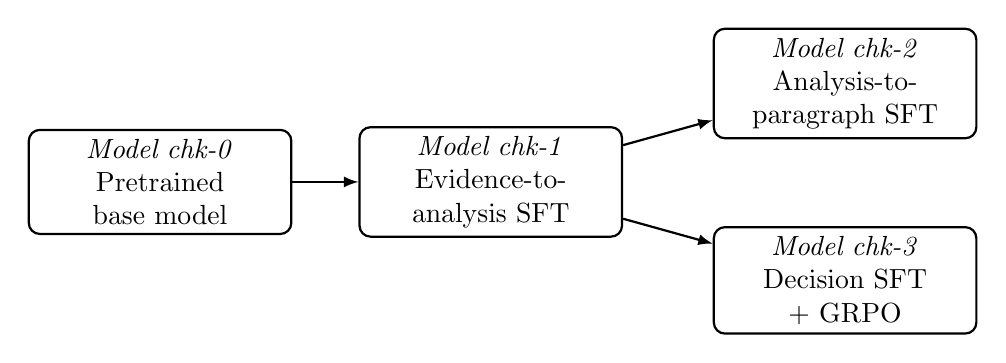
\begin{tikzpicture}[
        >=latex,
        model/.style={draw, rounded corners, align=center, text width=3.1cm,
            minimum height=1.25cm},
        every path/.style={->, thick}
    ]
        \node[model] (chk0) at (0,0)
            {\textit{Model chk-0}\\Pretrained base model};
        \node[model] (chk1) at (4.2,0)
            {\textit{Model chk-1}\\Evidence-to-analysis SFT};
        \node[model] (chk2) at (8.7,1.25)
            {\textit{Model chk-2}\\Analysis-to-paragraph SFT};
        \node[model] (chk3) at (8.7,-1.25)
            {\textit{Model chk-3}\\Decision SFT + GRPO};
        \draw (chk0) -- (chk1);
        \draw (chk1) -- (chk2);
        \draw (chk1) -- (chk3);
    \end{tikzpicture}
    \caption{Final paper-level training lineage.}
    \label{fig:ch2:training_stage1}
\end{figure}

Figure~\ref{fig:ch2:training_process} expands the lineage into the data and
optimization flows for analytical SFT and the two downstream tasks. The
retained diagrams use the original experimental identifiers: the
\textit{Model chk-3} and \textit{Model chk-4} labels printed in the graphics
correspond, respectively, to the paper-level \textit{Model chk-2} and
\textit{Model chk-3}. In addition, the ``Minutes'' box in the decision panel is
an earlier project-side shorthand; the finalized decision model receives the
target-neutral, pre-meeting analysis specified later in this section.

\begin{figure}[H]
    \centering
    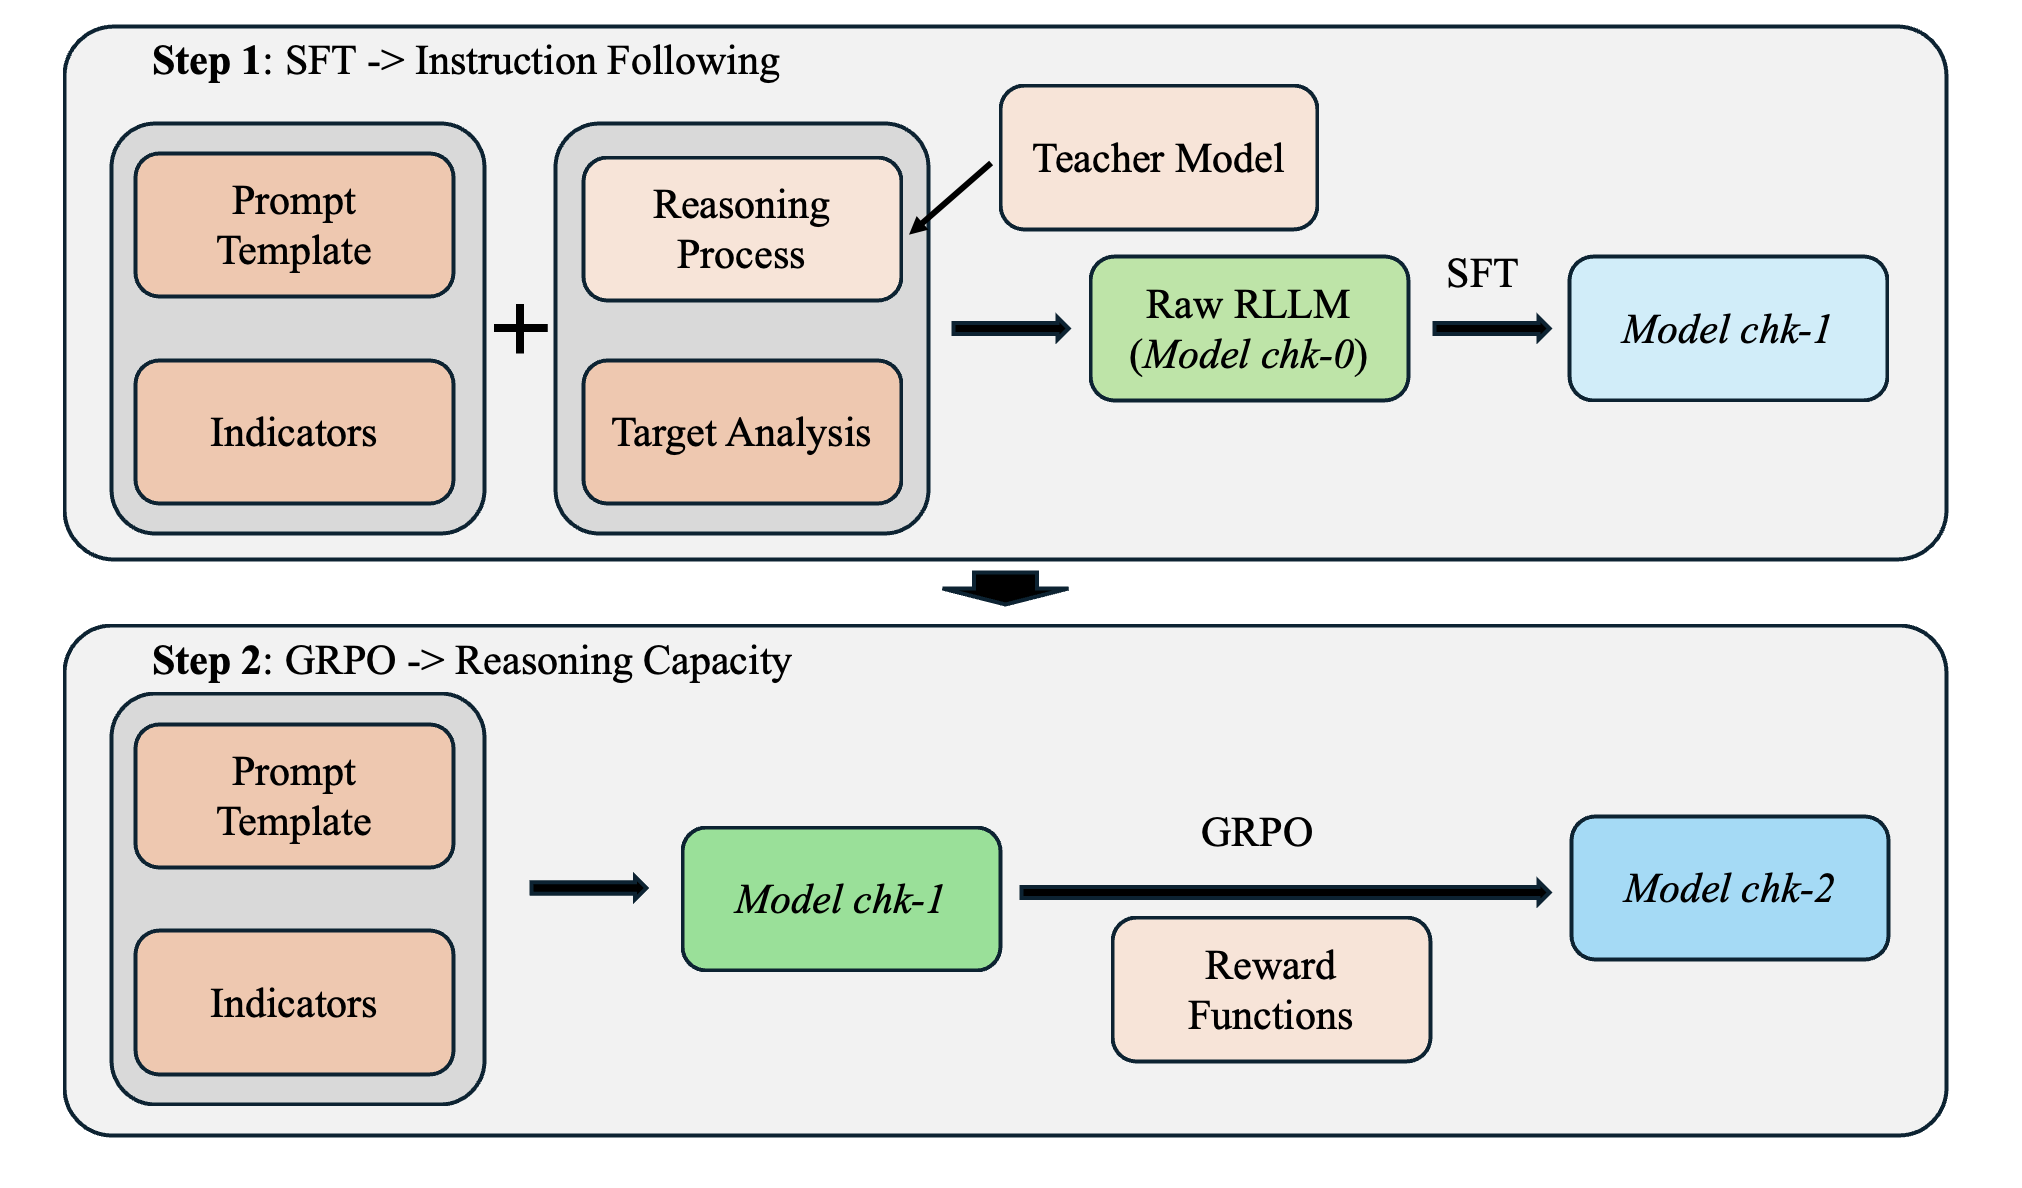
\includegraphics[width=\textwidth]{train/stage1.png}
    \par\medskip
    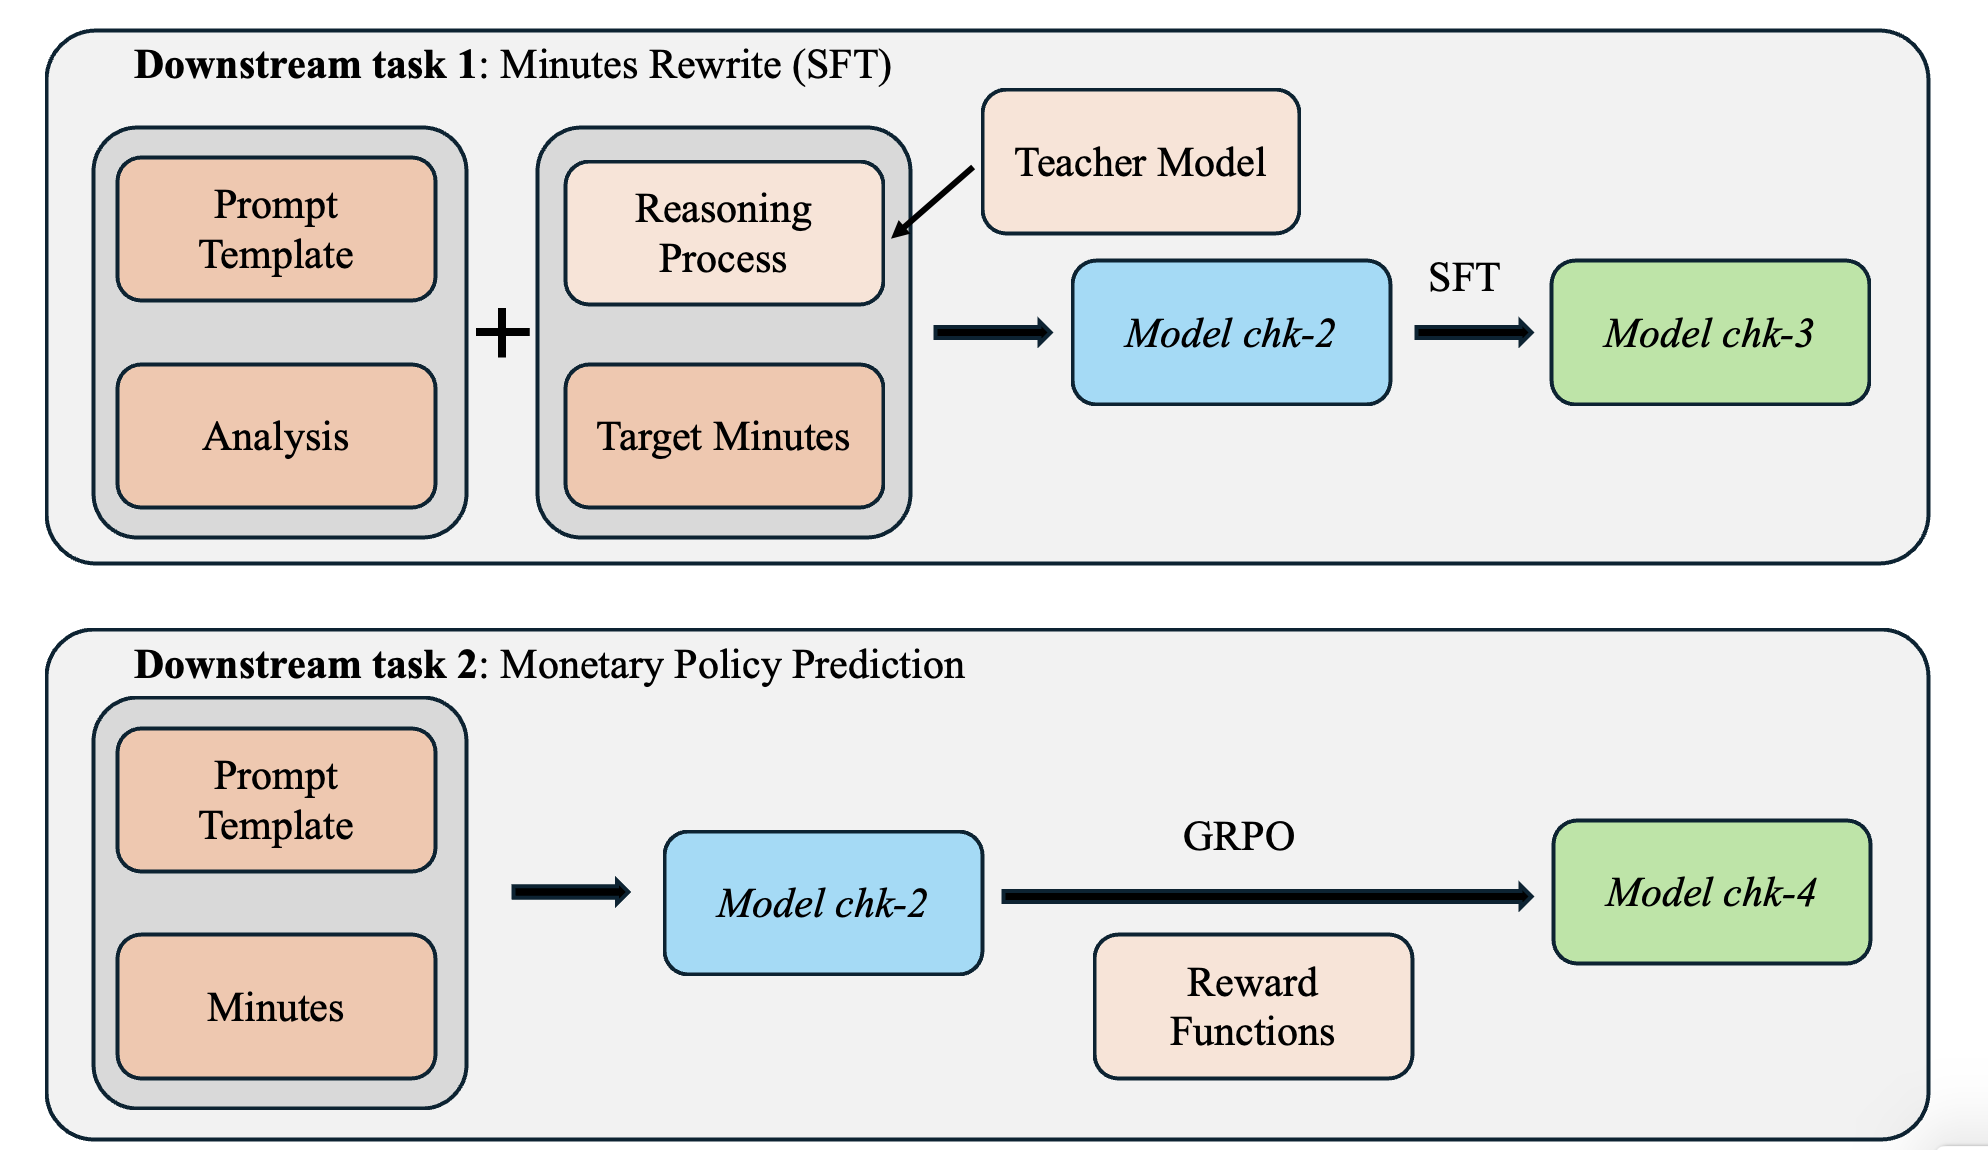
\includegraphics[width=\textwidth]{train/stage2.png}
    \caption{Overview of Two-step Training Process}
    \label{fig:ch2:training_process}
\end{figure}


%SFT
\paragraph*{Supervised fine-tuning.}
SFT adapts the model to the macro-financial tasks by learning from paired
prompts and reference completions. Each training example contains a system
instruction, a user prompt, and a target assistant response. The model is
optimized under teacher forcing, while parameter-efficient adapters reduce
the number of trainable parameters. Figure~\ref{fig:ch2:ft_detail} summarizes
this workflow.


\begin{figure}
    \begin{center}
        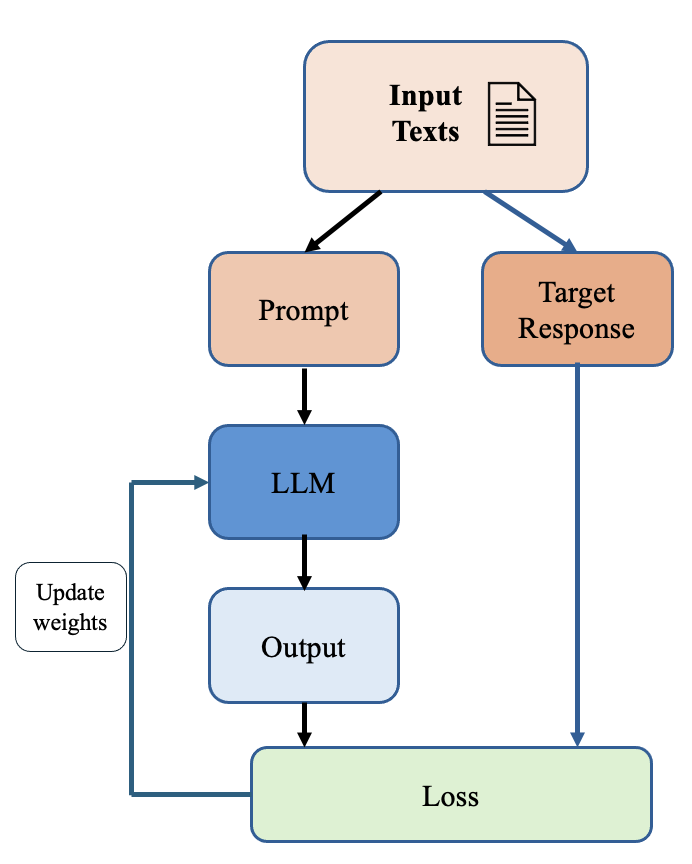
\includegraphics[width=0.3\textwidth]{Chapter2/Chapter2Figs/ft_detail.png}
      \end{center}
      \caption{Supervised fine-tuning workflow.}
      \label{fig:ch2:ft_detail}
\end{figure}



During SFT, let $x=(x_1,\ldots,x_M)$ denote the serialized prompt and
$y=(y_1,\ldots,y_N)$ the target assistant completion. At each target
position, the model predicts a distribution over the vocabulary conditional
on the prompt and preceding target tokens. The mean token-level negative
log-likelihood is
\begin{equation}
    \mathcal{L}_{\mathrm{SFT}}(\theta)
    =
    -\frac{1}{W}
    \sum_{t=1}^{N}
    w_t
    \log \pi_\theta\!\left(y_t\mid x,y_{<t}\right),
    \qquad
    W=\sum_{t=1}^{N}w_t,
\end{equation}
where $w_t\in\{0,1\}$ masks padding and any positions excluded from the
supervised objective. If every completion token is trained, $w_t=1$ and
$W=N$. Thus, SFT minimizes the negative log-probability assigned to the
reference completion; it does not compare a separately decoded response with
the target text.


%RL
\paragraph*{Reinforcement learning.}
Unlike SFT, policy optimization does not require a token-level reference
completion. In the decision task, however, the reference action remains
available to the deterministic reward function: the policy sees the prompt,
whereas the target direction and magnitude are used only to score sampled
completions.

Proximal Policy Optimization (PPO; \cite{schulman2017proximal}) stabilizes
policy-gradient updates by clipping the importance-sampling ratio. Let
$s_t=(q,o_{<t})$ be the token-generation state and define
\begin{equation*}
    \rho_t(\theta)
    =
    \frac{\pi_\theta(o_t\mid s_t)}
         {\pi_{\theta_{\mathrm{old}}}(o_t\mid s_t)}.
\end{equation*}
The clipped policy objective is
\begin{equation}
    \mathcal{J}_{\mathrm{PPO}}(\theta)
    =
    \mathbb{E}_t\!\left[
        \min\!\left(
            \rho_t(\theta)\widehat{A}_t,
            \operatorname{clip}
            \bigl(\rho_t(\theta),1-\epsilon,1+\epsilon\bigr)
            \widehat{A}_t
        \right)
    \right].
\end{equation}
Here, $\widehat{A}_t$ is an advantage estimate rather than the reward itself;
clipping constrains the policy ratio rather than rescaling the reward.




GRPO (\cite{shao2024deepseekmath}) removes the learned value function. For
each prompt $q$, the behavior policy samples a group
$\{o_i\}_{i=1}^{G}$, and the task reward assigns one terminal score
$R_i=R(q,y,o_i)$ to each completion. The group-relative advantage is
\begin{equation}
    \widehat{A}_i
    =
    \begin{cases}
    \displaystyle\frac{R_i-\overline{R}}{s_R+\eta}, & s_R>0,\\[7pt]
    0, & s_R=0,
    \end{cases}
    \qquad
    \overline{R}=\frac{1}{G}\sum_{j=1}^{G}R_j,
\end{equation}
where $s_R$ is the within-group reward standard deviation and $\eta>0$ is a
numerical stabilizer. The same completion-level advantage is applied to every
generated token in $o_i$. A group whose completions all receive the same
reward therefore supplies no group-relative learning signal.




For token $t$ of completion $i$, define
\begin{equation*}
    \rho_{i,t}(\theta)
    =
    \frac{\pi_\theta(o_{i,t}\mid q,o_{i,<t})}
         {\pi_{\theta_{\mathrm{old}}}(o_{i,t}\mid q,o_{i,<t})}.
\end{equation*}
A sampled per-token estimator for the KL regularizer is
\begin{equation*}
    \widehat{D}_{\mathrm{KL},i,t}
    =
    \frac{\pi_{\mathrm{ref}}(o_{i,t}\mid q,o_{i,<t})}
         {\pi_\theta(o_{i,t}\mid q,o_{i,<t})}
    -\log
    \frac{\pi_{\mathrm{ref}}(o_{i,t}\mid q,o_{i,<t})}
         {\pi_\theta(o_{i,t}\mid q,o_{i,<t})}
    -1.
\end{equation*}
Using
\begin{equation*}
    \ell_{i,t}(\theta)
    =
    \min\!\left(
        \rho_{i,t}(\theta)\widehat{A}_i,
        \operatorname{clip}
        \bigl(\rho_{i,t}(\theta),1-\epsilon,1+\epsilon\bigr)
        \widehat{A}_i
    \right)
    -\beta\widehat{D}_{\mathrm{KL},i,t},
\end{equation*}
the original sequence-normalized GRPO objective can be written as
\begin{equation}
    \mathcal{J}_{\mathrm{GRPO}}(\theta)
    =
    \mathbb{E}\!\left[
        \frac{1}{G}\sum_{i=1}^{G}
        \frac{1}{|o_i|}\sum_{t=1}^{|o_i|}
        \ell_{i,t}(\theta)
    \right].
\end{equation}

The completed decision run instead sets \texttt{loss\_type=dapo}. In this
trainer setting, DAPO denotes token-level loss aggregation: the losses are
normalized by the number of active completion tokens in the accumulated
training batch rather than separately by each completion length. If
$\mathcal{C}$ is the set of unmasked completions in that batch, the realized
aggregation is
\begin{equation}
    \mathcal{J}_{\mathrm{DAPO}}(\theta)
    =
    \mathbb{E}\!\left[
        \frac{\displaystyle
            \sum_{i\in\mathcal{C}}\sum_{t=1}^{|o_i|}\ell_{i,t}(\theta)}
             {\displaystyle
            \sum_{i\in\mathcal{C}}|o_i|}
    \right].
\end{equation}
This setting is related to the token-level aggregation proposed in DAPO
(\cite{yu2025dapo}), but it does not imply that the run adopted the complete
DAPO recipe. The realized configuration retained symmetric clipping and a KL
penalty; its numerical settings are reported with the decision-training
configuration below.





\subsection*{Analytical and Downstream Training}

\subsubsection*{Supervised Fine-tuning for the Analytical Model}

\paragraph*{Model chk-1.}
The first SFT stage adapts \textit{Model chk-0} to point-in-time
macro-financial analysis. Each supervised example is a pair
$(q_i,o_i^{\mathrm{SFT}})$, where $q_i$ is the model-visible prompt and
$o_i^{\mathrm{SFT}}=(c_i,a_i)$ is the reference assistant completion. Here,
$c_i$ denotes the reasoning prefix and $a_i$ the concise final analysis. This
distinction separates the model input from the supervision target. Training
for a small number of epochs limits, but does not eliminate, the risk that the
model memorizes task-specific wording.



Moreover, each LLM requires a model-specific message format, because tokenizers encode role boundaries differently. Explicit role labels are used specifically to distinguish the sections: the ``\texttt{System Prompt}'', ``\texttt{User Prompt}'', and ``\texttt{Assistant Response}''. Table. \ref{tab:ch2:input_template_for_llama3} presents the labels used by LLAMA3, where ``\prompttag{start\_header\_id}'' and ``\prompttag{end\_header\_id}'' wrap around the role labels indicating the message type. The label ``\prompttag{begin\_of\_text}'' signals the start of the conversation, while ``\prompttag{end\_id}'' denotes its end.



\begin{table}[h]
    \centering
    \footnotesize
    \begin{tabular}{p{0.98\textwidth}}
    \toprule
    \textbf{Special Labels for LLaMA 3:} \\
    \midrule
    \prompttag{begin\_of\_text} \\
    \prompttag{start\_header\_id} \textcolor{red}{system}\prompttag{end\_header\_id} \\
    \texttt{... System Prompts ...} \\
    \prompttag{start\_header\_id} \textcolor{red}{user}\prompttag{end\_header\_id} \\
    \texttt{... User Prompts ...} \\
    \prompttag{start\_header\_id} \textcolor{red}{assistant}\prompttag{end\_header\_id} \\
    \texttt{... Assistant Response ...} \\
    \prompttag{end\_id} \\
    \bottomrule
    \end{tabular}
    \caption{Input Template for LLAMA3}
    \label{tab:ch2:input_template_for_llama3}
\end{table}



\paragraph*{Reasoning boundary and final answer.}
The supervised completions follow the model's native reasoning-boundary
convention. A nonempty reasoning prefix $c_i$ is followed by exactly one
literal \texttt{</think>} marker and a nonempty final
answer $a_i$. Writing the boundary token as $b_{\mathrm{think}}$, the
serialized completion is
\begin{equation*}
    o_i=c_i\;\Vert\;b_{\mathrm{think}}\;\Vert\;a_i,
\end{equation*}
where $\Vert$ denotes string concatenation,$b_{\mathrm{think}} = \texttt{</think>} $. The semantic form of $a_i$ is task-specific: prose for \textit{Models chk-1} and \textit{chk-2}, and a decision object for \textit{Model chk-3}. 






\subsubsection*{Further Training for Downstream Tasks}

We adapt \textit{Model chk-1} separately for two downstream tasks. SFT on
analysis-to-FOMC-Minutes-style paragraph pairs produces \textit{Model chk-2}.
A separate branch uses decision SFT followed by GRPO to produce
\textit{Model chk-3}, which
predicts the direction and magnitude of a federal funds rate action.


\paragraph*{FOMC-Minutes-Style Paragraph Rewriting (\textit{Model chk-2})}

The Minutes-rewriting branch begins from the exact-merged \textit{Model chk-1}  and applies task-specific supervised fine-tuning to learn an analysis-to-paragraph transformation. 

First of all, because official FOMC Minutes often contain substantial details absent from the corresponding economic-analysis passages used as training inputs, treating the Minutes directly as targets would create misaligned supervision. We therefore used a teacher model to reconstruct a factually complete, de-styled analysis from each Official Minutes paragraph, ensuring that the student learns stylistic rewriting rather than supplying missing facts.

Then, for each training instance, the student model receives a fixed system instruction and a user message containing the analysis to be rewritten. Under teacher forcing, the target completion consists of a fidelity-planning reasoning section, one literal \texttt{</think>} boundary, and a single rewrote formal FOMC Minutes paragraph. The optimization objective therefore emphasizes the preservation of claims, quantities, dates, directions, comparisons, and uncertainty while adapting the output to the institutional style and structure of the FOMC Minutes. 




\paragraph*{Monetary Policy Decision Making (\textit{Model chk-3})}

The monetary-policy decision branch begins independently from the exact-merged \textit{Model chk-1} and proceeds through decision-specific SFT followed by GRPO. During SFT, the model receives a fixed system instruction and a user message containing a target-neutral pre-meeting analysis. The supervised completion consists of a qualitative dual-mandate rationale, one literal \texttt{</think>} boundary, and a terminal object specifying the policy direction and magnitude. GRPO then initializes from decision SFT checkpoint, retains the same model-facing prompt, action space, and response contract, and optimizes the parser-contingent decision proxy reward. 



\subsection*{Technique for Parameter-Efficient Fine-Tuning (PEFT)}

Full-parameter fine-tuning updates every model parameter and must retain the
associated gradients and optimizer states. Parameter-efficient fine-tuning
instead freezes the pretrained weights and optimizes a much smaller set of
task-specific parameters.

We use Low-Rank Adaptation (LoRA; \cite{hu2021lora}). For a pretrained linear
transformation with weight
$W\in\mathbb{R}^{d_{\mathrm{out}}\times d_{\mathrm{in}}}$, LoRA represents
the trainable update as
\begin{equation}
    W'=W+\Delta W,
    \qquad
    \Delta W=\frac{\alpha}{r}BA,
\end{equation}
where $A\in\mathbb{R}^{r\times d_{\mathrm{in}}}$,
$B\in\mathbb{R}^{d_{\mathrm{out}}\times r}$, and
$r\ll\min(d_{\mathrm{in}},d_{\mathrm{out}})$. The pretrained matrix $W$
remains frozen; only the low-rank factors are optimized.

Quantized Low-Rank Adaptation (QLoRA; \cite{dettmers2024qlora}) combines LoRA
with a quantized frozen base model; its 4-bit NormalFloat (NF4) representation
is distinct from generic FP4. The final training record for \textit{chk-2}
checkpoint 50 verifies NF4 QLoRA training with double quantization and
BF16 compute and storage, using a rank-32, $\alpha=64$ LoRA adapter with
dropout 0.05 on \texttt{q\_proj},
\texttt{k\_proj}, \texttt{v\_proj}, \texttt{o\_proj},
\texttt{gate\_proj}, \texttt{up\_proj}, and \texttt{down\_proj}. The main
text-similarity evaluation loads this adapter over the exact-merged
\textit{chk-1} checkpoint 200 parent in BF16 without inference quantization;
the \textit{chk-2} adapter itself remains active rather than being merged.
An adapter may remain
separate from its parent model or be merged for deployment; merging does not
by itself reduce the size of the resulting base-sized model.




\subsection{Training Hyperparameters}\label{ch2:sec:parameter}

Table~\ref{tab:ch2:training_hyperparameters_archive} reports checkpoint
identities and configuration values. 

\begin{table}[H]
    \centering
    \footnotesize
    \setlength{\tabcolsep}{3pt}
    \renewcommand{\arraystretch}{1.16}
    \begin{tabularx}{\textwidth}{@{}
        >{\centering\arraybackslash}p{0.08\textwidth}
        >{\centering\arraybackslash}p{0.08\textwidth}
        >{\raggedright\arraybackslash}p{0.18\textwidth}
        >{\raggedright\arraybackslash}p{0.18\textwidth}
        >{\raggedright\arraybackslash}X
    @{}}
        \toprule
        \textbf{Model} & \textbf{Stage} & \textbf{Initialization} &
        \textbf{Selected Point} &
        \textbf{Configuration} \\
        \midrule
        \textit{chk-1} & SFT & \textit{chk-0} & Checkpoint 200 selected and
        exact-merged & Final evaluation records fix the artifact identity;
        full training settings are not bound in the current record set. \\
        \textit{chk-2} & SFT & Exact-merged \textit{chk-1} checkpoint 200 &
        Checkpoint 50 selected by the validation-probe rule; active adapter &
        NF4 QLoRA $r=32$, $\alpha=64$, dropout 0.05; learning rate
        $10^{-6}$; three epochs (60 optimizer steps); completion-only loss.
        Selection evidence is reported in Appendix~\ref{app:checkpoint_selection}. \\
        \textit{chk-3} & SFT & Exact-merged \textit{chk-1} checkpoint 200 &
        Checkpoint 38 initializes GRPO & 211 unique meetings, 312 physical
        training rows. \\
        \textit{chk-3} & GRPO & Decision SFT checkpoint 38 & Run completed at
        step 468; checkpoint 450 used for evaluation &
        \texttt{loss\_type=dapo}; within-group scaling; four generations per
        prompt; generation batch 8; temperature 0.7; top-$p$ 0.9;
        $\beta=0.04$; $\epsilon=0.2$; prompt/completion limits 2,560/1,536;
        truncated completions masked; sole proxy reward
        \texttt{decision\_dense\_v3} with external weight 1.0. \\
        \bottomrule
    \end{tabularx}
    \caption{Paper-level model lineage and verified subset of the training configuration.}
    \label{tab:ch2:training_hyperparameters_archive}
\end{table}




% we are able to construct two types of mandate-specific sentiment indicators: PN and Tone indicators 
% predicting important economic variables. An adaptive Bayesian approach


% Estimation results show that both policy decisions and communication have economically large
% and highly significant effects on the exchange rates, with the surprise component of statements account-
% ing for most of the explainable variation in exchange rate returns in response to monetary policy

% induce “higher than
% normal” volatility across different asset classes. 

% I find that minutes sentiments have a statistically significant
% association with the fed funds futures rate and the U.S. dollar’s valuation.


% First,
% I examine the financial market effect of the release of FOMC
% minutes on U.S. asset prices (Treasury rates, stock prices, and
% U.S. dollar exchange rates) using a high-frequency, event-study
% analysis.



% as Rosa (2013) explains, the minutes, however, still receive a
% significant amount of attention because they are longer and contain more information and nuances about the policy meetings.

% examining their importance also offers a more independent analysis compared to the policy statements since minutes releases do not
% overlap with announcements about monetary policy changes.

% how the sentiments of these policy documents impact the predictability of financial market changes.



\section{Model Evaluation Methods}\label{ch2:sec:application}


In this section, we evaluate the archived model outputs with a focus on reliability and evidence boundaries. Because LLMs are probabilistic generators, a central concern is hallucination: content that is unsupported by the provided inputs or misaligned with real-world facts. \citet{huang2025survey} distinguish between factuality hallucination and faithfulness hallucination. This chapter mainly targets the latter, asking whether generated policy text remains grounded in the conditioning indicators and whether downstream validation results justify the claims attached to each checkpoint.




LLM evaluation can be broadly classified as reference-based or reference-free. Firstly, reference-based evaluation compared the model's outputs with the target outputs under the same prompts. Scores are used to quantitatively measure the difference, for instance, F1 Score measures the accuracy for classification tasks, BLEU(\cite{papineni2002bleu}) measures string match accuracy and BERTScore (\cite{zhang2019bertscore}) measures the token embeddings' similarity. Noticeably, reference outputs are required for reference-based evaluation. For reference-free evaluation, no reference is needed for this method. The evaluation is usually model-based, such as regression-based validation result between the input prompts and the outputs, LLM-as-Judge scoring, and human assessment.


LLM evaluation can be broadly classified into reference-based and reference-free evaluation. First, reference-based evaluation compares the model’s outputs with target outputs generated under the same prompts. Scores are then used to quantitatively measure the differences between them. For example, the F1 score measures classification accuracy, BLEU \cite{papineni2002bleu} measures string-level overlap, and BERTScore \cite{zhang2019bertscore} measures semantic similarity based on token embeddings. Notably, reference outputs are required for reference-based evaluation. By contrast, reference-free evaluation does not require predefined target outputs. It is usually model-based or judgement-based, including regression-based validation between input prompts and outputs, LLM-as-Judge scoring, and human assessment.


Because high-quality reference answers are available for several tasks in this study, we primarily use reference-based evaluation. More specifically, we examine four dimensions: 1) \textbf{textual similarity}, 2) \textbf{input grounding under leave-one-out masking}, 3) \textbf{exploratory sentiment--return validation}, and 4) \textbf{decision prediction benchmarked against historical, econometric, and market-implied baselines}.

The first two dimensions address faithfulness to the conditioning inputs. The latter two provide downstream checks on whether the synthetic texts preserve economically meaningful signals. Because the canonical split is meeting-level but random rather than chronological (Section~\ref{ch2:sec:the-dataset}), these downstream results should be interpreted as held-out meeting validation rather than as definitive evidence about forward-only time-series generalization.

\begin{table}[htbp]
    \centering
    \footnotesize
    \begin{tabular}{p{0.18\textwidth} p{0.18\textwidth} p{0.17\textwidth} p{0.18\textwidth} p{0.22\textwidth}}
        \toprule
        \textbf{Experiment} & \textbf{Checkpoint(s)} & \textbf{Evaluation Data} & \textbf{Main Metrics} & \textbf{Conclusion Boundary} \\
        \midrule
        Textual similarity & Checkpoint-3 vs. Checkpoint-2 & Held-out Minutes test meetings & Cosine Similarity, BERTScore & Evidence about stylistic/semantic closeness on a meeting-level random holdout, not chronological extrapolation \\
        Leave-one-out masking & Backbone-0 or Checkpoint-3 depending on generation setup & Held-out masking prompts derived from test meetings & $\Delta_i$ under leave-one-out masking & Evidence about local prompt sensitivity, not exact Shapley attribution \\
        Sentiment--return validation & Synthetic Minutes generated from Checkpoint-3 & Synthetic Minutes produced from the held-out Minutes split & Bootstrap coefficient distributions, $t$-statistics & Exploratory directional validation only; weak significance still limits stronger market-relevance claims \\
        Decision prediction & Backbone-0, Checkpoint-4, majority baseline, lag-1 baseline, multinomial logit, market-implied baseline & Deduplicated held-out decision meetings & Exact match, accuracy, balanced accuracy, macro-F1, confusion matrix & Comparison to LLM, historical, econometric, and market-implied baselines on the same held-out meetings \\
        \bottomrule
    \end{tabular}
    \caption{Experiment Scope and Interpretation Boundaries}
    \label{tab:ch2:experiment_scope}
\end{table}



\subsection*{Evaluation Methods}


\subsubsection*{Textual Similarity}

% Cosine Similarity
To start with, the textual similarity targets comparing the similarity between the target output and the generated output using mathematical distance, such as the Levenshtein Similarity Ratio (\cite{levenshtein1966binary}) and Cosine Similarity (\cite{tanguy2016natural}). The Levenshtein Similarity Ratio replies on the Levenshtein Distance to measure the minimum number of strings that need to be edited from the generated output to the required output. Furthermore, some other metrics driven from the idea of ``n-grams'', such as the Recall-Oriented Understudy for Gisting Evaluation score (ROGUE score, \cite{lin2004rouge}), provide an grammatical-level measurement than the word-level Levenshtein Similarity Ratio. These methods are useful at the age of ``Bag-Of-Word (BOG)''.

However, with the development of LLM, researchers can take advantage of the embeddings from the LLM rather than the one-hot key of ``BOG''. The embeddings can convert the ``word'' into tokens that encoded more semantic information than the one-hot key. Therefore, the Cosine Similarity provides a more accurate estimation of the semantic similarity between two texts. Here, we will use the \textit{sentence-level} \textbf{Cosine Similarity} as our first metric to evaluate the text similarity of outputs. Cosine Similarity ranges from 0 to 1, where a value of 1 indicates a perfect similarity between the two texts, while a value of 0 signifies that the texts are highly different from each other.

The metric helps in determining how well the generated text aligns with the expected content in terms of both meaning and context. For example, \cite{aynetdinov2024semscore}, \cite{kim2024comparison}, and \cite{yauney2023data} used the Cosine Similarity as a benchmark when evaluating the LLM's performance.

Cosine similarity is estimated by the cosine of the angle between two non-zero vectors. It is defined as the dot product of the two vectors divided by the product of their magnitudes. This mathematical operation helps in quantifying how closely the generated text aligns with the target text in terms of meaning and content. We utilize the ``tokenizer'' and the ``hidden layers'' from the LLAMA3 model to convert the response texts into vector representations, denoted as $Y$ for the target text and $\hat{Y}$ for the generated text.


%%% text embedding calculation

% tokens = [2, 1, 3]
% text_embedding = [[0.111, 0.232131, 0.41414, 0.2412424, 0.1424, 0.444, 0.99]
%                     [0.5151, 0.52215, 0.232132, 0.223232, 0.535151, 0.23231, 0.515151]
%                     [0.2155252, 0.2223, 0.54331, 0.321313, 0.14222, 0.421555, 0.535252]]
% mean pooling = [0.23131, 0.222, 0.23213, 0.325325, 0.532555, 0.535325, 0.23232, 0.424141]

% | 模型          | hidden_size | num_hidden_layers |
% | ----------- | ----------- | ----------------- |
% | BERT-base   | 768         | 12                |
% | Llama-7B    | 4096        | 32                |
% | GPT-3 small | 12288       | 96                |

% google-bert 768, [https://huggingface.co/google-bert/bert-base-uncased/blob/main/config.json]
% gemini3-27b 5376,, [https://huggingface.co/google/gemma-3-27b-it/blob/main/config.json]
% Deepseek-r1 7168,[https://huggingface.co/deepseek-ai/DeepSeek-R1/blob/main/config.json]
% llama3.1-70b  8192,




Compared with the ``one-hot encoding'' used in the ``Bag-of-Words'' model, the text embeddings employed in large language models (LLMs) offer two significant advantages. On the one hand, text embeddings employ a tokenizer to map the input text into a sequence of dense vectors, $\mathbf{h}_i \in \mathbb{R}^{m\times 1}$, where $i = 1, 2, ..., n$ corresponds to each token in the text, and $m$ denotes the hidden-layer dimension, rather than high-dimensional binary representations. On the other hand, the hidden layers within the LLM transform each token vector into a contextualized embedding by encoding both semantic meaning and positional information.

Noticeably, the hidden layer size ($m$) is different for different models. Generally, a larger hidden dimension allows the model to capture more fine-grained semantic information. For example, Google BERT (110M parameters) has a hidden size of 768 \cite{googlebert}, Gemini 3-27B has a hidden size of 5,376 \cite{googlegemini3}, and LLaMA 3.1-70B uses a hidden size of 8,192 \cite{metallama3}.


Furthermore, after the encoding stage, there is a pooling stage aimed at adjusting the dimension of text embedding matrix ($\mathbf{H} \in \mathbb{R}^{M\times N} = [\mathbf{h_1}, \mathbf{h_2}, ..., \mathbf{h_N}]$) to 1 ($\mathbf{H'} \in {\mathbb{R}^{M\times 1}}$). Then, this adjusted text embedding is a vector representation of the input text. Common pooling strategies include mean pooling, max pooling, and weighted-sum pooling. 

% During the pooling stage, token embeddings are aggregated—typically by averaging across all tokens—to produce a single fixed-length vector representing the entire input text. Common pooling strategies include mean pooling, max pooling, and weighted-sum pooling. 

% First, mean pooling computes the average embedding across all tokens:

% \begin{equation}\label{eq:ch2:mean_pooling}
%     h'_{j} = \frac{1}{N} \sum_{i=1}^{N} h_{ij}
% \end{equation}

% where $h_{ij}$ denotes the j-th dimension of the i-th token embedding.

% Second, max pooling selects the maximum value across all tokens for each embedding dimension:

% \begin{equation}\label{eq:ch2:max_pooling}
%     h'_{j} = Max(h_{1j}, h_{2j}, ..., h_{Nj})
% \end{equation}


% Finally, weighted-sum pooling computes a weighted average of token embeddings:

% \begin{equation}\label{eq:ch2:weight_sum_pooling}
%         h'_{j} = \frac{1}{N} \sum_{i=1}^{N} w_{i,j}h_{ij} 
% \end{equation}
% where $w_{ij}$ are non-negative weights satisfying $\sum_{i=1}^{N} w_{ij} = 1$ . In practice, attention weights from a pre-trained transformer are often used as $w_{ij}$.
 
To balance the effect of all the tokens, in this study, we adopt mean pooling. Max pooling tends to overemphasize a small number of highly activated tokens, while weighted-sum pooling can be dominated by tokens with disproportionately large attention weights. Mean pooling therefore provides a more stable and balanced document representation for the cosine-similarity calculations used in this chapter. 


Therefore, the cosine similarity score, denoted as $Cos_{Y, \hat{Y}}$, is then calculated as follows:


\begin{equation*}
    Cos_{Y, \hat{Y}} = \frac{Y \cdot \hat{Y}}{\|Y\|_2 \|\hat{Y}\|_2}
\end{equation*}


where $Y$ and $\hat{Y}$ are sentence embeddings for the reference and generated texts, and $\|\cdot\|_2$ denotes the Euclidean norm (e.g., $\|Y\|_2=\sqrt{y_1^2+y_2^2+\cdots+y_N^2}$).


% According to the distribution theory, 
Finally, drawing from distributional semantics theory (\cite{firth1957linguistics}, \cite{sahlgren2008distributional}), words with similar meanings tend to occur in similar contexts and thus have similar distributions in the vector space. Therefore, we hypothesize that texts with higher semantic likeness will exhibit a greater cosine similarity. 
% This theory, first proposed by \cite{firth1957linguistics} and later expanded upon in the context of distributional semantics by \cite{sahlgren2008distributional}, suggests that words can be represented as real-valued vectors that encapsulate their linguistic meanings. 

% For instance, 


% BERTScore 

% On the other hand, in addition to Cosine Similarity, which serves as a \textit{sentence-level} metric measuring the similarity between entire texts, we also employ \textbf{BERTScore} (\cite{zhang2019bertscore}), a metric designed to capture \textit{token-level} semantic similarity using cosine similarity as its underlying distance measure.
%
% Specifically, for each token $\hat{y}_j$ in the target (reference) output $\hat{Y}$, BERTScore identifies the maximum cosine similarity with respect to all candidate tokens $y_i$ in the generated response $Y$. These maximal token-level similarities are then aggregated to construct three complementary evaluation metrics: \textit{Recall} ($BertScore^{Recall}$), \textit{Precision} ($BertScore^{Precision}$), and the harmonic mean of the two, the \textit{F1 score} ($BertScore^{F1}$).
%
% Firstly, Recall (Eq.(\ref{eq:ch2:bert_recall})) quantifies the proportion of tokens in the reference text that are semantically represented in the generated response. Then, Precision (Eq.(\ref{eq:ch2:bert_precision})) measures the proportion of tokens in the generated response that semantically match those in the reference text. Finally, the F1 Score (Eq.(\ref{eq:ch2:bert_f1})) is calculated as the harmonic mean of precision and recall, thereby providing a balanced measure of semantic alignment between the generated and reference texts.
%
% \begin{equation}\label{eq:ch2:bert_recall}
%     BertScore^{Recall} = \frac{1}{\|Y\|}\sum_{y_i \in Y} \underset{\hat{y}_j \in \hat{Y}}{\text{max }}y_i ^{\text{T}}\hat{y}_j
% \end{equation}
%
% \begin{equation}\label{eq:ch2:bert_precision}
%     BertScore^{Precision} = \frac{1}{\|\hat{Y}\|}\sum_{\hat{y}_i \in Y} \underset{y_j \in \hat{Y}}{\text{max }}\hat{y}_i ^{\text{T}}y_j
% \end{equation}
%
% \begin{equation}\label{eq:ch2:bert_f1}
%     BertScore^{F1} = 2 \frac{BertScore^{Recall} + BertScore^{Precision}}{BertScore^{Recall}\cdot BertScore^{Precision}}
% \end{equation}
% [CH2-109][Original Start]
% On the other hand, in addition to Cosine Similarity (a sentence-level metric), we also employ \textbf{BERTScore} (\cite{zhang2019bertscore}), which measures \textit{token-level} semantic similarity using contextual embeddings and cosine similarity.
%
% Let $Y=\{y_i\}$ denote the set of token embeddings in the generated response and $\hat{Y}=\{\hat{y}_j\}$ denote the set of token embeddings in the reference (target) text. BERTScore computes \textit{Precision} by matching each candidate token to its most similar reference token, and \textit{Recall} by matching each reference token to its most similar candidate token. The \textit{F1 score} then balances the two.
%
% \begin{equation}\label{eq:ch2:bert_precision}
%     BertScore^{Precision} = \frac{1}{\|Y\|}\sum_{y_i \in Y} \max_{\hat{y}_j \in \hat{Y}} y_i^{\text{T}}\hat{y}_j
% \end{equation}
%
% \begin{equation}\label{eq:ch2:bert_recall}
%     BertScore^{Recall} = \frac{1}{\|\hat{Y}\|}\sum_{\hat{y}_j \in \hat{Y}} \max_{y_i \in Y} \hat{y}_j^{\text{T}}y_i
% \end{equation}
%
% \begin{equation}\label{eq:ch2:bert_f1}
%     BertScore^{F1} = \frac{2\cdot BertScore^{Precision}\cdot BertScore^{Recall}}{BertScore^{Precision}+BertScore^{Recall}}
% \end{equation}
%
%
% \begin{equation*}
%     \begin{split}
%         &Cos_{FT} - Cos_{Base} > 0 \\
%         &BertScore^{Recall}_{FT} - BertScore^{Recall}_{Base} > 0 \\
%         % &BertScore^{Precsion}_{FT} - BertScore^{Precision}_{Base} > 0\\
%         % [Codex 修改版] 2026-02-26: 修正拼写。
%         &BertScore^{Precision}_{FT} - BertScore^{Precision}_{Base} > 0\\
%         &BertScore^{F1}_{FT} - BertScore^{F1}_{Base} >0 
%     \end{split}
% \end{equation*}
% [CH2-109][Original End]
On the other hand, in addition to Cosine Similarity, which serves as a \textit{sentence-level} metric, we also employ \textbf{BERTScore} (\cite{zhang2019bertscore}), a metric designed to capture \textit{token-level} semantic similarity using cosine similarity as its underlying distance measure.

More specifically, for each token $\hat{y}_j$ in the target (reference) output $\hat{Y}$, BERTScore identifies the maximum cosine similarity with respect to all candidate tokens $y_i$ in the generated response $Y$. These maximal token-level similarities are then aggregated to construct three complementary evaluation metrics: \textit{Recall} ($BertScore^{Recall}$), \textit{Precision} ($BertScore^{Precision}$), and the harmonic mean of the two, the \textit{F1 score} ($BertScore^{F1}$).


Let $Y=\{y_i\}$ denote the set of token embeddings in the generated response and $\hat{Y}=\{\hat{y}_j\}$ denote the set of token embeddings in the reference (target) text. BERTScore computes \textit{Precision} by matching each candidate token to its most similar reference token, and \textit{Recall} by matching each reference token to its most similar candidate token. Finally, the F1 Score (Eq.(\ref{eq:ch2:bert_f1})) is calculated as the harmonic mean of precision and recall, thereby providing a balanced measure of semantic alignment between the generated and reference texts:

\begin{equation}\label{eq:ch2:bert_precision}
    BERTScore^{Precision} = \frac{1}{\|Y\|}\sum_{y_i \in Y} \max_{\hat{y}_j \in \hat{Y}} y_i^{\text{T}}\hat{y}_j
\end{equation}

\begin{equation}\label{eq:ch2:bert_recall}
    BERTScore^{Recall} = \frac{1}{\|\hat{Y}\|}\sum_{\hat{y}_j \in \hat{Y}} \max_{y_i \in Y} \hat{y}_j^{\text{T}}y_i
\end{equation}

\begin{equation}\label{eq:ch2:bert_f1}
    BERTScore^{F1} = \frac{2\cdot BERTScore^{Precision}\cdot BERTScore^{Recall}}{BERTScore^{Precision}+BERTScore^{Recall}}
\end{equation}


Overall, we propose the following hypotheses for cosine similarity and BERTScore:

\begin{equation*}
    \begin{split}
        &Cos_{FT} - Cos_{Base} > 0 \\
        &BERTScore^{Recall}_{FT} - BERTScore^{Recall}_{Base} > 0 \\
        &BERTScore^{Precision}_{FT} - BERTScore^{Precision}_{Base} > 0\\
        &BERTScore^{F1}_{FT} - BERTScore^{F1}_{Base} > 0
    \end{split}
\end{equation*}


% [CH2-119][Original Start]
% where subscripts $FT$ and $Base$ denote the fine-tuned and baseline models. The hypothesis is that fine-tuning increases semantic alignment with the target text. A statistically significant result would indicate that the fine-tuned model has effectively learned additional semantic and contextual information through the fine-tuning process.
% [CH2-119][Original End]
where subscripts $FT$ and $Base$ denote the two archived checkpoints being compared in a given experiment. In the textual-similarity results below, these correspond to Checkpoint-3 and Checkpoint-2. A statistically significant positive difference indicates that the adapted checkpoint is semantically closer to the target text than its archived comparator.


%%%%% end of text similarity


\subsubsection*{Input Grounding under Leave-one-out Masking}

Apart from similarity, we also want the generated output to reflect the conditioning indicators rather than generic policy language. The archived repository does not contain an exact subset-based Shapley attribution implementation for this chapter's reported tables. Instead, the implemented test is a \textbf{leave-one-out masking similarity test}: one indicator is removed from the prompt, the section is regenerated, and the change in similarity to a target text is recorded.

Formally, let $\mathcal{P}=\{p_1,\ldots,p_n\}$ denote the full set of indicator prompts and let $o(\cdot)$ denote the generated section under a given prompt set. For indicator $p_i$, we define the leave-one-out masking score as:

\begin{equation}\label{eq:ch2:loo_masking}
    \Delta_i = Cos\big(o(\mathcal{P}), o_{target}\big) - Cos\big(o(\mathcal{P}\setminus\{p_i\}), o_{target}\big)
\end{equation}

where $Cos(\cdot)$ is computed on sentence embeddings of the generated section and $o_{target}$ denotes the target text used for evaluation. In this chapter, $o_{target}$ is either (i) the synthetic section generated under the full prompt or (ii) the corresponding actual FOMC Minutes section. A positive $\Delta_i$ means that removing the indicator lowers similarity to the target, while a negative $\Delta_i$ means that removing the indicator moves the output \textit{closer} to the target. The latter case is substantively important because it signals that some indicators may be noisy, redundant, or used in a direction that does not improve the target section.

Operationally, we hold all non-masked prompt content fixed and generate one additional output for each masked indicator. This is therefore a local sensitivity test, not an expected-marginal-contribution estimator over all possible prompt subsets. The interpretation is correspondingly narrower: the exercise reveals which indicators the model appears to rely on under the archived prompt template, but it does not provide a full cooperative-game attribution.

Because we compare both synthetic targets and actual-Minutes targets, the interpretation differs across the two cases. Against synthetic targets, a positive $\Delta_i$ indicates reliance on the indicator for reproducing the model's own unmasked output. Against actual Minutes, both positive and negative values are informative: a positive value suggests that the indicator helps recover the reference section, while a negative value indicates that the model's use of that indicator may not improve fidelity to the historical text.

\begin{equation*}
\Delta_i > 0
\end{equation*}


%%%% end of shapley

\subsubsection*{Exploratory Validation using Synthetic Texts}

% [CH2-081][Original Start]
% In this test, we evaluate the model’s simulation capacity by conducting empirical analyses on the synthetic text it generates. The current literature has confirmed the impact of the release of FOMC Minutes on the financial market, for instance, \cite{rosa2013financial} found that the release of the Minutes significantly increases the volatility of the U.S. asset prices, including treasury rate, equity market index and the exchange rate. \cite{rosa2011high} found that both the statements and the policy decisions have significant effects on the exchange rate market. \cite{huang2021economic} applied an adaptive Bayesian text mining approach, and confirmed the predictive power of the sentiments of FOMC's text in important economic variables. \cite{tadle2022fomc} confirmed the sentiments contained in the Minutes have significantly impacts on the fed funds futures rate and U.S. dollars exchange rate. Therefore, to confirmed the statistically significant of our fine-tuned LLM, we conduct empirical tests on our synthetic Minutes.
% [CH2-081][Original End]
This test evaluates simulation quality through downstream empirical models. Prior studies show that FOMC communication affects financial markets (\cite{rosa2013financial}; \cite{rosa2011high}; \cite{huang2021economic}; \cite{tadle2022fomc}). Here, however, the role of the regression is more modest: we use it as an exploratory check on whether sentiment extracted from synthetic Minutes moves coefficients in the direction of the benchmark estimates. Given the random meeting-level split design and the weak conventional significance levels reported later, this exercise should not be read as a definitive validation of market relevance.


% [CH2-082][Original Start]
% To assess this, we adopt the empirical strategy from \cite{tadle2022fomc}, which examines how FOMC Minutes influence market expectations regarding monetary policy. Specifically, first of all, we apply the main regression model (Eq.\ref{eq:ch2:sentiment_reg})from their study, which investigates the relationship between sentiment scores derived from FOMC communications and movements in interest and exchange rates. In our case, we use the same regression framework to test whether sentiment extracted from our synthetic minutes yields similar effects on financial market variables.
% [CH2-082][Original End]
We follow the empirical design in \citet{tadle2022fomc} and estimate Eq.~\ref{eq:ch2:sentiment_reg}, which links communication sentiment to interest-rate and exchange-rate movements. In our setting, sentiment is extracted from synthetic Minutes.


\begin{equation}\label{eq:ch2:sentiment_reg}
    p^f_t = \lambda p^f_{t-1} + \alpha + \beta_{Z_t^M} Z_t^M+ \beta_{Z_{t-1}^M} Z_{t-1}^M + \beta_{Z_t^S} {Z_t}^S + \beta_{VIX_t}VIX_t + \beta_{Y_t}Y_t + \phi_t 
\end{equation}


% [CH2-083][Original Start]
% where $p^f_t$ is the price for the Federal Fund Rate Future contract $f$ at time $t$. $VIX_t$ is the log change of the Volatility Index (VIX), $Z_t^M$ and $Z_t^S$ are the sentiment scores extracted from the Minutes and Statements, $Y_t$ is the monthly time effect, and $\phi_t$ is the error term.
% [CH2-083][Original End]
where $p_t^f$ is the price of Federal Funds futures contract $f$ at time $t$, $VIX_t$ is the log change in VIX, $Z_t^M$ and $Z_t^S$ are sentiment scores from Minutes and statements, $Y_t$ captures month effects, and $\phi_t$ is the error term. In the empirical implementation, futures prices and related market series are obtained from WRDS and Refinitiv DataScope Select; the DataScope component is retrieved programmatically using \texttt{datascope\_apis} with token-managed asynchronous extraction and file-integrity checks (Section~\ref{ch2:sec:the-dataset}).



% where pft is the asset price in period t of the daily futures contract f. VIXt is the log percentage change of the adjusted closing price of VIX on day t. It serves as a measure of the perceived financial market riskiness and therefore has been found to have significant influence on the changes in asset prices. Furthermore, Y is a vector of month-of-year indicator variables used to implement month of year fixed effects while ϕt is the error term of the specification.


% Our second empirical test focuses on the effect of the “words” used in the FOMC Minutes on the equity market. \cite{cieslak2021economics} found that the FOMC incorporates information from stock market performance into its monetary policy decisions. Their study confirmed that language in the Minutes related to equity market conditions is significantly correlated with subsequent changes in the Federal Funds Rate. Therefore, we analyze whether the textual content of the synthetic Minutes can similarly predict FFR changes. More specifically, we will employ the following regression for our analysis:


% \begin{equation}\label{eq:ch2:word_reg}
%     \begin{split}
%             \Delta FFR_m &= \alpha + \beta_{FFR_{m-1}}FFR_{m-1} + \beta_{FFR_{m-2}}FFR_{m-2} + \beta_{FFR_{m-3}}FFR_{m-3} \\
%             &+ \beta_{\#Stocks_{m}^{-}}\#Stocks_{m}^{-} + \beta_{\#Stocks_{m-1}^{-}}\#Stocks_{m-1}^{-} \\
%             &+ \beta_{\#Stocks_{m}^{+}}\#Stocks_{m}^{+} + \beta_{\#Stocks_{m-1}^{+}}\#Stocks_{m-1}^{+} \\
%             & + \beta_{Doc.length_m} + \phi_m \\
%     \end{split}
% \end{equation}


% where $\Delta FFR_m$ denotes the change in the Federal Funds Rate at FOMC meeting $m$, which is measured in basis points (BPS), and $FFR_{m-1}$, $FFR_{m-2}$, and $FFR_{m-3}$ represent the Federal Funds Rates from the three preceding meetings. $\#Stocks_{m}^{-}$ and $\#Stocks_{m}^{+}$ indicate the number of “Negative” and “Positive” equity-related tones identified in the Minutes for meeting $m$, respectively. Finally, $Doc.length_m$ refers to the total word count of the Minutes document, included to normalize for document length.



Following the empirical test, we conduct a bootstrap procedure to estimate the distribution of the $\beta$ coefficients. In the present chapter, these bootstrap distributions are used to compare direction and relative magnitude across checkpoints, not to claim that synthetic text robustly reproduces the full market effects of historical Minutes.



%%%% end of statistical significant



% The
% relation could be coincidental in the sense that the Fed views the stock market as
% uninformative but the econometrician finds it has explanatory power for target
% changes because the stock market is correlated with variables that drive the
% Fed’s decision-making. Alternatively, the Fed may perceive stock returns as
% informative and therefore react to them. This could be due to stock returns
% being viewed as a driver of the economy, or due to them being viewed
% as a useful predictor of economic variables the Fed cares about, notably
% growth

%  the Fed does pay attention to the stock
% market directly, we perform a textual analysis of the minutes and transcripts
% of FOMC meetings

%  participants (the chair, vice-chair, other
% governors, and regional Reserve Bank presidents)

% \cite{gardner2022words}




\subsubsection*{Decision-making Accuracy}
Finally, at each Federal Open Market Committee (FOMC) meeting, the Committee votes on monetary policy decisions—most notably the target range of the Federal Funds Rate (FFR), also referred to as the Federal Funds Target Rate. Once the target rate is established, the Federal Reserve employs a range of monetary policy instruments to steer the effective FFR toward the desired level by adjusting the supply of reserves within the banking system. These instruments include open market operations (purchasing and selling U.S. government securities), the Interest on Reserve Balances (IOR), and the Overnight Reverse Repurchase Agreement (ON RRP) facility. Consequently, FOMC decisions exert a direct influence on the interest rate market, with subsequent spillover effects on exchange rates and equity markets.

The final stage of our empirical evaluation assesses the model’s simulation ability to predict monetary policy decisions, specifically changes in the Federal Funds Rate, based on macroeconomic and financial indicators. In this context, each FOMC meeting represents a decision-making instance in which the Committee determines the appropriate policy stance in response to evolving economic conditions and market developments.


A substantial body of literature has confirmed the significant impact of FOMC decisions on financial markets. For example, \cite{lucca2015pre} documented notable pre-announcement returns in the S\&P 500 Index since 1994, suggesting market anticipation of FOMC actions. \cite{cieslak2019stock} showed that unexpected policy decisions led to a pronounced decline in the equity premium between 1994 and 2016. Similarly, \cite{madeira2019effect} found that stock prices respond significantly to policy announcements. Further, \cite{bodilsen2021asset} and \cite{liu2022recovering} established a positive relationship between the equity risk premium and portfolio beta around FOMC announcements.


Furthermore, the Federal Funds Futures market plays a pivotal role in the broader financial system. For example, as of May 23, 2025, the 30-Day Federal Funds Futures contract accounted for approximately 5.97\% of total open interest in the U.S. derivatives market—representing a 37.9\% year-over-year increase amid rising economic uncertainty.

% [CH2-120][Original Start]
% Given that our fine-tuned model is capable of emulating the analytical style of the FOMC, it can also infer monetary policy actions based on meeting discussions. Therefore, we further evaluate the model’s decision-making accuracy in predicting changes to the Federal Funds Rate (FFR). This evaluation aims to provide insights into the model’s decision-making capabilities and further explore its potential to simulate realistic monetary policy behavior.
% [CH2-120][Original End]
Decision prediction is treated here as a downstream stress test rather than as a definitive forecasting claim. The objective is to examine whether analytical checkpoints retain enough policy-relevant signal to infer coarse FFR actions from meeting context, and whether that signal survives comparison with historical, econometric, and market-implied baselines on a common held-out meeting set.



% Given these findings, we evaluate the predictive accuracy of our fine-tuned model in replicating FOMC policy decisions. This evaluation aims to provide insights into the model’s decision-making capabilities and to further examine its potential for simulating monetary policy behavior.


% To this end, we first extracted historical FFR changes from the Federal Reserve Bank of New York between 2000 and 2025 (Table~\ref{tab:ch2:ffr_changes}). The changes mainly laid between increase 75 basis points (bps) and decrease 75 basis points. Therefore, we designed a list of potential changes (Table~\ref{tab:ch2:vote_choice}) and ask the model to choose one using the prompt in Table~\ref{tab:ch2:prompt_for_decision_prediction}.


% Given these findings, we evaluate the predictive accuracy of our fine-tuned model in replicating FOMC policy decisions. This evaluation aims to provide insights into the model’s decision-making capabilities and further explore its potential to simulate realistic monetary policy behavior.


% [CH2-121][Original Start]
% To this end, we first extracted historical FFR changes from the Federal Reserve Bank of New York spanning 2000 to 2025 (Table~\ref{tab:ch2:ffr_changes}). The changes mainly ranged between increases and decreases of 75 basis points (bps). Based on this historical distribution, we constructed a list of potential FFR changes (Table~\ref{tab:ch2:vote_choice}) and prompted the model to select the most appropriate option using the format outlined in Table~\ref{tab:ch2:prompt_for_decision_prediction}, where the \texttt{current\_analysis} represents the other sections from the FOMC minutes. Finally, we assessed the model’s decision-making performance by comparing its predictions to the actual FOMC outcomes, thereby evaluating its accuracy in replicating historical monetary policy decisions.
% [CH2-121][Original End]
To this end, we first extracted historical FFR changes from the Federal Reserve Bank of New York spanning 2000 to 2025 (Table~\ref{tab:ch2:ffr_changes}). Based on this historical distribution, we constructed a list of candidate actions (Table~\ref{tab:ch2:vote_choice}) and prompted the model to select one option using the format in Table~\ref{tab:ch2:prompt_for_decision_prediction}, where \texttt{current\_analysis} denotes the non-decision sections of the Minutes. In the results section, archived model outputs are then evaluated on a meeting-date-deduplicated set and compared not only with another checkpoint but also with majority-class and lag-1 action baselines.


\begin{table}[htbp]
    \centering
    \footnotesize
    \begin{minipage}[t]{0.48\textwidth}
        \centering
        \begin{tabular}{c c}
            \toprule
            Rate Change (bps) & Frequency \\
            \midrule
            0    & 6,177 \\
            25   & 31 \\
            -50  & 15 \\
            -25  & 12 \\
            75   & 4 \\
            50   & 2 \\
            -75  & 2 \\
            \bottomrule
        \end{tabular}
        % [CH2-090][Original Start]
        % \caption{Daily Federal Fund Rate Changes (in BPS) from Jan 1, 2000 to May 9, 2025}
        % [CH2-090][Original End]
        \caption{Daily Federal Funds Rate Changes (in bps), January 1, 2000 to May 9, 2025}
        \label{tab:ch2:ffr_changes}
    \end{minipage}
    \hfill
    \begin{minipage}[t]{0.48\textwidth}
        \centering
        \begin{tabular}{l}
            \toprule
            Target Vote Choices \\
            \midrule
            Raise by 100 basis points \\
            Raise by 75 basis points \\
            Raise by 50 basis points \\
            Raise by 25 basis points \\
            No change \\
            Cut by 25 basis points \\
            Cut by 50 basis points \\
            Cut by 75 basis points \\
            Cut by 100 basis points \\
            \bottomrule
        \end{tabular}
        \caption{Choices for Target Vote}
        \label{tab:ch2:vote_choice}
    \end{minipage}
\end{table}







\section{Empirical Results}\label{ch2:sec:result}
% [CH2-084][Original Start]
% In this section, we will attempt to generate the FOMC Minutes using a Large Language Model (LLM). Fine-tuning large pre-trained models is a highly effective method for adapting general-purpose LLMs to specific content tasks. This technique enables the model to conform to a particular style, affecting not only the output format but also the semantics. Furthermore, we will employ various approaches to evaluate the performance of the fine-tuned model in this specific task.
% [CH2-084][Original End]
This section reports training and downstream evaluation results for FOMC-Minutes generation. We assess both optimization dynamics (loss/reward trajectories) and task performance under text-based and economics-based criteria.


\subsection*{Model Training Results}

% \subsubsection*{Stage 1 Supervised Fine-Tuning Results}
% [Codex 修改版] 2026-02-26: 与前文 “2-Step Training Plan” 术语一致，统一用 Step 1/Step 2 描述核心训练流程。
\subsubsection*{Step 1: Supervised Fine-Tuning (SFT) Results}

% [CH2-085][Original Start]
% In this section, we will try to fine-tune the base model (\textbf{LLAMA3B-8}). The number of total trainable parameters is 3,407,872 out of 8,051,232,768 total parameters with one adopter (only 0.0423\% trainable rate).
% [CH2-085][Original End]
% [CH2-108][Original Start]
% Step 1 fine-tunes the base model (\textbf{LLaMA3-8B}). We train 3,407,872 parameters out of 8,051,232,768 total parameters (trainable ratio: 0.0423\%).
% [CH2-108][Original End]
% [CH2-122][Original Start]
% Step 1 fine-tunes the base model (\textbf{LLaMA 3-8B}). We train 3,407,872 parameters out of 8,051,232,768 total parameters (trainable ratio: 0.0423\%).
% [CH2-122][Original End]
Step 1 fine-tunes Backbone-0 (\textbf{DeepSeek-R1-Distill-Llama-8B}). We train 3,407,872 parameters out of 8,051,232,768 total parameters (trainable ratio: 0.0423\%).

% [CH2-086][Original Start]
% Firstly, we conduct Supervised Fine-Tuning on the model to enhance the instruction-following ability. We trained the model with 3 epochs and 2,346 steps. Each epoch will go though all 3,128 training dataset and the gradient will be update every 4 generations, which makes it 2,346 steps in total. Additionally, the model will calculate the loss for the evaluation dataset every 20 steps. Finally, Figure~\ref{fig:ch2:stage1_sft_loss} illustrates the training loss and the corresponding evaluation loss.
% [CH2-086][Original End]
SFT is trained for 3 epochs (2,346 optimization steps). Each epoch covers 3,128 training samples, with gradient accumulation every 4 generations. Evaluation loss is logged every 20 steps. Figure~\ref{fig:ch2:stage1_sft_loss} reports training and evaluation loss.


\begin{figure}[htbp]
    \begin{center}
            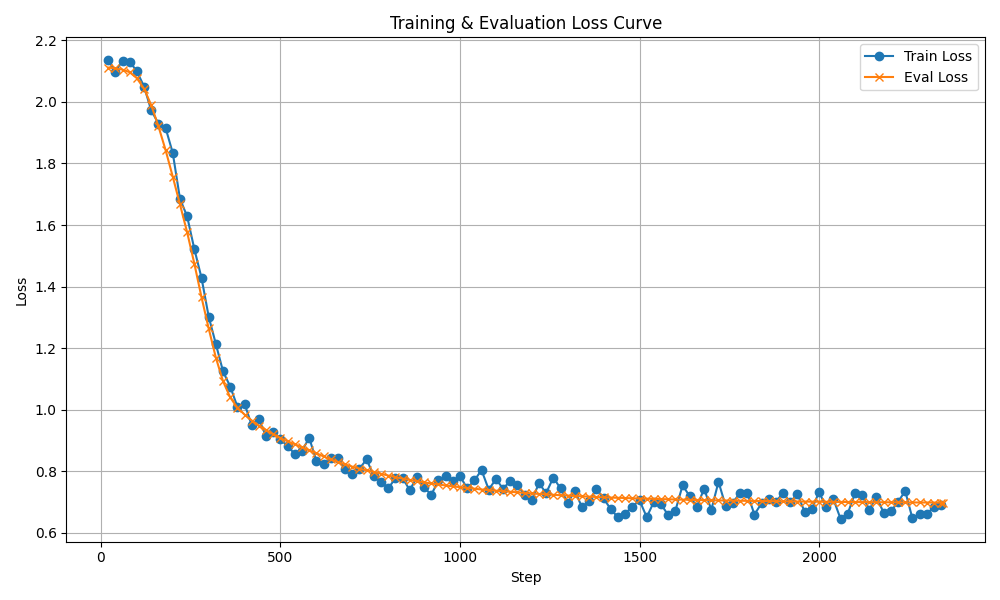
\includegraphics[width=0.9\textwidth]{Chapter2/Chapter2Figs/stage1_train/training_curve_sft_20250521.png}
            % \caption{Training Loss and Evaluation Loss for Stage 1 Supervised Fine-Tuning}
            % [Codex 修改版] 2026-02-26
            \caption{Training Loss and Evaluation Loss for Step 1 (SFT)}
            \label{fig:ch2:stage1_sft_loss}
    \end{center}
\end{figure}


% [CH2-087][Original Start]
% Initial experiment starts with 3 epochs, as shown in Figure \ref{fig:ch2:stage1_sft_loss}. During the period, the training loss decreased from 2.1504 (at Step = 20) to 0.6913 (at Step = 2340), Simultaneously, the evaluation loss converged from 2.1193 (at Step 20) to 0.7097 after 1,560 steps and remained stable ending with 0.6984 at step = 2340. Notably, while the training loss continued to decline after 1,340 iterations, the evaluation loss stabilized, indicating the potential onset of overfitting, where the model might become excessively specialized to the training data and lose its generalization capability. Overfitting can significantly degrade a model's utility outside the training environment.
% [CH2-087][Original End]
As shown in Figure~\ref{fig:ch2:stage1_sft_loss}, training loss declines from 2.1504 (step 20) to 0.6913 (step 2340). Evaluation loss decreases from 2.1193 to 0.7097 by step 1,560 and ends at 0.6984. After roughly step 1,340, training loss continues to fall while evaluation loss plateaus, which is consistent with mild overfitting risk.


% \subsubsection*{Stage 2 Group Relative Policy Optimization Results}
% After SFT, in the second stage, we conduct Reinforcement Learning (RL) via Group Relative Policy Optimization (GRPO) to the model to enhance the model's analytical ability. Followed by Section \ref{ch2:sec:model_train:rl}, we implemented the \textit{accuracy reward} to evaluate the model's answer and the \textit{reasoning reward} to track the reasoning process. We assigned same weights for both reward functions, the final reward is the weighted average of these two rewards. Figure~\ref{fig:ch2:stage2_grpo_reward} illustrates the 20-step rolling average of the total training reward during Stage 2 GRPO, along with the corresponding upper and lower bounds representing $\pm$1 standard deviation at each step.
% [Codex 修改版] 2026-02-26
\subsubsection*{Step 2: Group Relative Policy Optimization (GRPO) Results}
% [CH2-123][Original Start]
% After SFT, in Step 2, we conduct Reinforcement Learning (RL) via Group Relative Policy Optimization (GRPO) to further enhance analytical and reasoning quality. Following Section~\ref{ch2:sec:model_train:rl}, we implement an \textit{accuracy reward} to evaluate the final analysis and a \textit{reasoning reward} to evaluate the reasoning trajectory. We assign equal weights to the two reward components, and Figure~\ref{fig:ch2:stage2_grpo_reward} plots the 20-step rolling average of the total training reward during GRPO with $\pm$1 standard deviation bands.
% [CH2-123][Original End]
After SFT, Step 2 applies GRPO to further enhance analytical and reasoning quality. Following Section~\ref{ch2:sec:model_train:rl}, the canonical analysis run uses a \textit{format reward}, an \textit{answer reward}, and a \textit{reasoning reward}. The corresponding weights are $0.2$, $0.4$, and $0.4$, respectively. Figure~\ref{fig:ch2:stage2_grpo_reward} plots the 20-step rolling average of the total training reward during GRPO with $\pm$1 standard deviation bands.



\begin{figure}[htbp]
    \begin{center}
            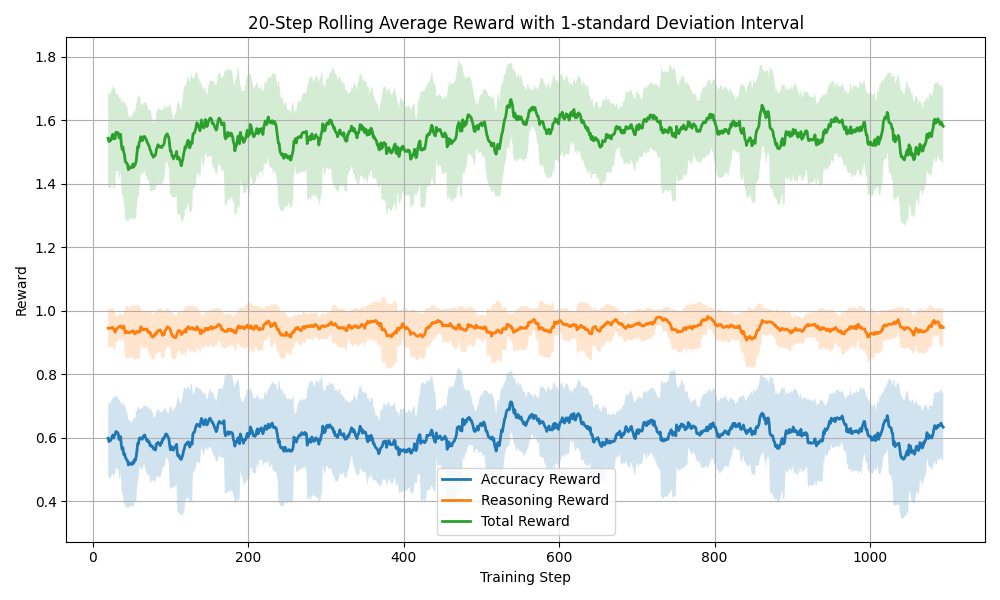
\includegraphics[width=0.9\textwidth]{Chapter2/Chapter2Figs/stage1_train/trainer_state_grpo_stage1_20250517.png}
            % \caption{20-Step Rolling Average of Training Reward for Stage 2 GRPO, with $\pm$1-Standard Deviation Intervals}
            % [Codex 修改版] 2026-02-26
            \caption{20-Step Rolling Average of Training Reward for Step 2 (GRPO), with $\pm$1-Standard Deviation Intervals}
            \label{fig:ch2:stage2_grpo_reward}
    \end{center}
\end{figure}


% [CH2-124][Original Start]
% In this step, the model was trained for one epoch. The training log over 1,094 steps demonstrates increasing stability in the reward metrics, particularly in the \textit{Accuracy Reward}. The 20-step rolling average of the \textit{Total Reward} showed a steady rise from approximately 0.70 to around 0.78, before stabilizing with minor fluctuations near 0.756, with block-level averages ranging from 0.76 to 0.79. The \textit{Reasoning Reward} remained consistently high, averaging around 0.95 and only occasionally dipping to approximately 0.85, indicating a robust and reliable chain-of-thought generation. In contrast, the \textit{Accuracy Reward} improved from 0.44 in the early stages to above 0.70, before stabilizing in the 0.60-0.65 range—suggesting enhanced precision in final responses, though with some potential for further improvement.
% [CH2-124][Original End]
In this step, the model was trained for one epoch. The training log over 1,094 steps demonstrates increasing stability in the reward metrics, particularly in the \textit{answer reward}. The 20-step rolling average of the \textit{Total Reward} rose from roughly 0.70 to around 0.78 before stabilizing near 0.756, with block-level averages ranging from 0.76 to 0.79. The \textit{reasoning reward} remained consistently high, often near 0.95, while the \textit{answer reward} improved from about 0.44 in the early stage to the 0.60--0.70 range later in training. Taken together, the logged trajectory is consistent with a more stable analytical checkpoint, although the reward plot alone does not establish out-of-sample gains.


% Moreover, reward volatilities exhibited signs of convergence. The 200-step rolling standard deviation declined from 0.0641 to 0.0584 for the \textit{reasoning reward}, from 0.1331 to 0.1250 for the \textit{accuracy reward}, and from 0.1573 to 0.1449 for the \textit{total reward}. These reductions in variability further confirm the model’s improved analytical consistency following training.

% 
% To assess the effectiveness of the Group Relative Policy Optimization (GRPO) training in Stage 1, we analyze the evolution of reward signals logged throughout the training trajectory. The reward structure comprises two components: the reasoning reward, which captures the logical coherence of the model’s generated explanation, and the answer reward, which measures the factual correctness or format alignment of the final answer.


% In this step, the model was trained for one epoch. The training log over 1,094 steps demonstrates increasing stability in the reward metrics. The 20-step rolling average of the \textit{Total Reward} showed a steady rise from approximately 0.70 to around 0.78, before stabilizing with minor fluctuations near 0.756

% After more than 1,000 recorded training steps, the reasoning reward consistently remains high, frequently exceeding 0.9 and often approaching the upper bound of 1.0. This indicates that the fine-tuned language model (LLM) rapidly acquires and maintains strong performance in producing logically structured thought processes. By contrast, the answer reward exhibits greater variance, oscillating between 0.3 and 0.8. Such variability suggests that while the model’s reasoning may be sound, its ability to render syntactically or semantically precise answers remains an area for further refinement.

% 



% [CH2-088][Original Start]
% In summary, with only 0.042\% of parameters left trainable, the \textbf{LLAMA-3-8B} model demonstrated measurable improvements following the two-step training process. Supervised Fine-Tuning (SFT) reduced the training loss to 0.69 over three epochs, while the validation loss stabilized around 0.70, which indicates strong instruction-following capability. Subsequently, the observed decline in reward volatility and the upward trend in reward scores during Group Relative Policy Optimization (GRPO) confirmed enhancements in the model's analytical performance. Overall, the combined approach of instruction tuning followed by reinforcement learning effectively improved both reasoning consistency and answer quality
% [CH2-088][Original End]
In summary, with only 0.042\% trainable parameters, the two-step process yields measurable gains. SFT improves supervised fit, and GRPO improves reward-aligned reasoning stability. Together, these stages improve both reasoning consistency and final-answer quality.

% [Codex 修改版] 2026-04-17: 恢复 Checkpoint-3 的正式训练结果段，并使用当前归档中的 loss / trainer_state 数字。
\subsubsection*{Checkpoint-3: Minutes-style Alignment Results}

Checkpoint-3 corresponds to the downstream Minutes-style SFT branch built on top of Checkpoint-1. The archived run uses 1,113 alignment-training samples and converges over 1,668 optimization steps (2.996 epochs). The archived trainer-state and train/eval summaries show a first logged training loss of 2.0127 at step 20 and a first logged evaluation loss of 2.0589. By the end of training, the merged artifact records a train loss of 1.1045, and the final logged evaluation loss declines to 0.9443 at step 1,660 (the saved evaluation summary reports 0.9442). This trajectory indicates that the Minutes-style branch learns a materially tighter mapping from analytical summaries to official-section prose than in the early iterations.

\begin{figure}[htbp]
    \begin{center}
            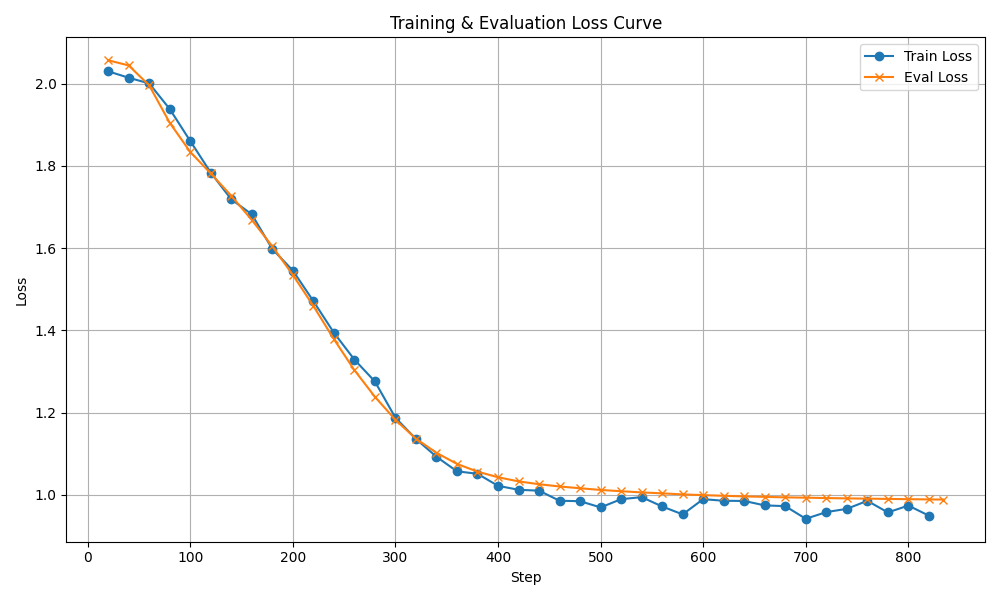
\includegraphics[width=0.9\textwidth]{Chapter2/Chapter2Figs/training_curve_synthetic_20250526.png}
            \caption{Training Loss and Evaluation Loss for Checkpoint-3 Minutes-style Alignment SFT}
            \label{fig:ch2:checkpoint3_sft_loss}
    \end{center}
\end{figure}

Figure~\ref{fig:ch2:checkpoint3_sft_loss} shows a smooth decline in both training and evaluation loss, with the evaluation curve flattening near the end of training rather than diverging sharply. This is consistent with the later textual-similarity tables: Checkpoint-3 is the branch that should be credited for the improvement in Minutes-style rewriting, not the generic analysis GRPO checkpoint.

% [Codex 修改版] 2026-04-17: 补写 Checkpoint-4 的训练归档摘要，并明确评估模型来自 checkpoint-1100。
\subsubsection*{Checkpoint-4: Decision-specific GRPO Training Summary}

The decision-specific branch evaluated later in this chapter is separate from Checkpoint-3. In the canonical pipeline, Checkpoint-4 is exported to \texttt{output/training/main/merged/decision\_grpo} after GRPO training from the decision adapter directory. The saved trainer state records the rate-accuracy reward, rate-format reward, KL term, completion length, and optimizer progress in machine-readable form, so the downstream decision results can be tied back to a specific runtime configuration rather than to an ambiguously named historical checkpoint.

Taken together, the downstream branches should be read asymmetrically: Checkpoint-3 provides the stronger evidence on textual alignment, while Checkpoint-4 is a separate policy-direction specialist whose performance must be judged only on the archived decision exports.




% \subsubsection*{Stage 2 Results}

% In this section, we further fine-tuned the model for the task of synthetic FOMC Minutes generation. The training dataset consisted of 1,113 question-answer (Q\&A) pairs. The model was trained for 3 epochs with gradient accumulation every 2 steps and an effective batch size of 1. The total number of optimization steps was 1,668.

% Training began with an initial loss of 2.0127, while the evaluation loss at step 20 was 2.0589. As training progressed, the loss steadily decreased, reaching a value of 0.9494 at step 820, accompanied by an evaluation loss of 0.9895. Figure~\ref{fig:ch2:stage2_sft} illustrates the training and evaluation loss trajectories throughout the process. These results indicate that the model successfully converged to a stable performance level.


% \begin{figure}[htbp]
%     \begin{center}
%             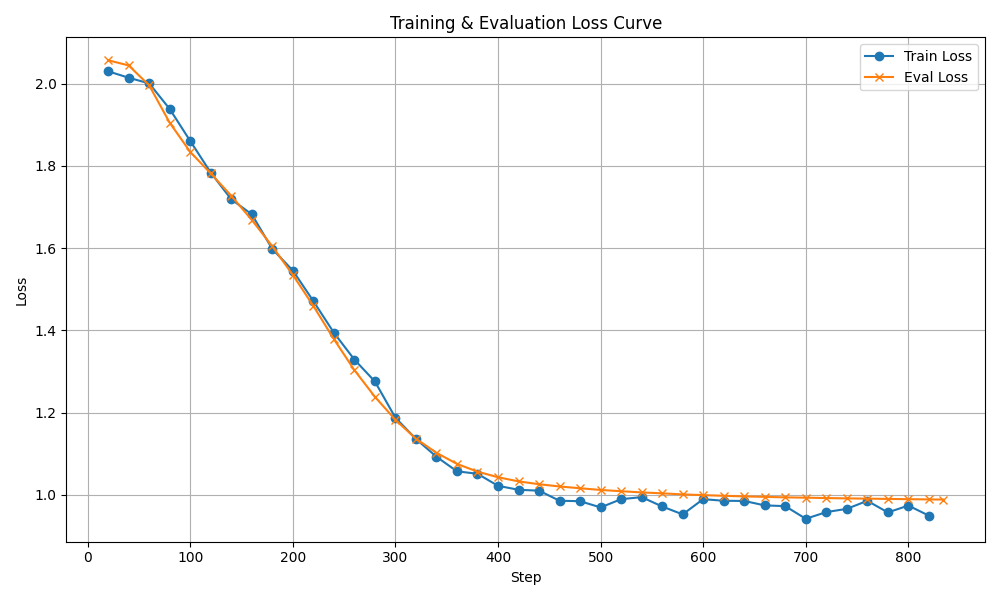
\includegraphics[width=0.9\textwidth]{Chapter2/Chapter2Figs/training_curve_synthetic_20250526.png}
%             \caption{Training Loss and Evaluation Loss for Stage 2 Synthetic Text Supervised Fine-Tuning}
%             \label{fig:ch2:stage2_sft}
%     \end{center}
% \end{figure}



% \subsection*{Policy Prediction Training Results}

% In this section, we applied Group Relative Policy Optimization (GRPO) to fine-tune the model in predicting the monetary policy decision, specifically the vote for the change of the Federal Fund Rate (FFR). Here, we employed two reward functions for optimization, \textit{``Vote Accuracy Reward''} and \textit{``Vote Format Reward''}. The \textit{``Total Reward''} is summed of these two rewards. Figure~\ref{fig:ch2:stage2_grpo} illustrated the rolling average total rewards with a window of 20 steps after 1940-step training. 


% \begin{figure}[htbp]
%     \begin{center}
%             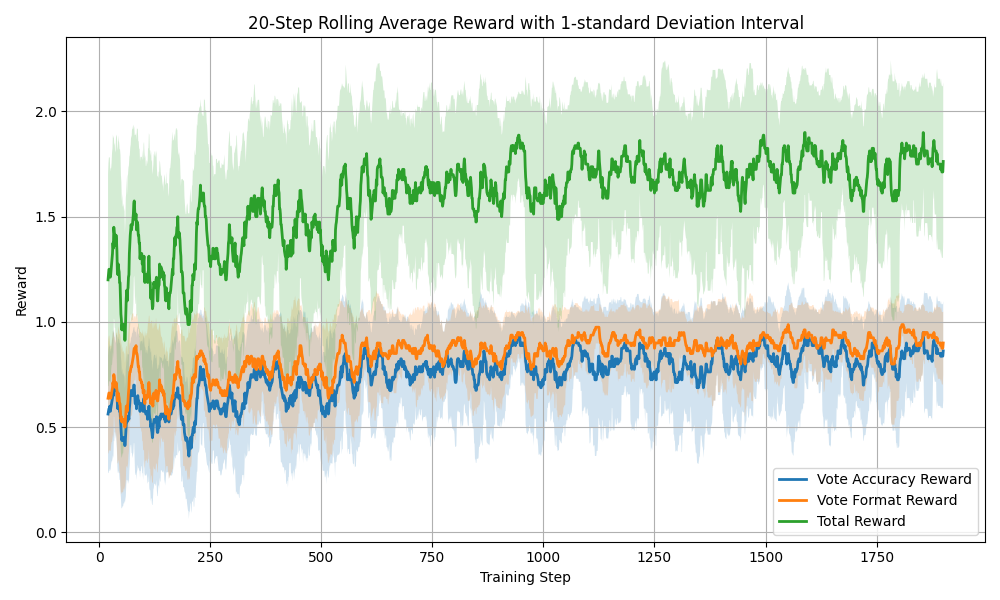
\includegraphics[width=0.9\textwidth]{Chapter2/Chapter2Figs/stage2_train/trainer_state_grpo_stage2_1900_20250527.png}
%             \caption{Rolling Average Rewards for Stage 2 Decision-Making Reinforcement Learning with $\pm$1-Standard Deviation Intervals}
%             \label{fig:ch2:stage2_grpo}
%     \end{center}
% \end{figure}



% % 
% For this stage of training, we initiated the process with a total of 5 epochs and 1,940 training steps. Throughout the training trajectory, both the format reward and accuracy reward demonstrated consistent upward trends, indicative of effective early-stage learning and successful policy optimization. By step 1,200, the rolling standard deviations for each reward component had notably decreased, reflecting improved stability in model behavior and convergence toward higher-reward regions of the parameter space. This reduction in reward volatility underscores the model’s growing consistency and reliability in generating policy-aligned voting decisions.

% Importantly, after step 1,200, the total reward plateaued, and no further significant upward trend was observed. To mitigate the risk of overfitting and ensure generalization, we selected the model checkpoint at step 1,200 (corresponding to epoch 2.0) as the final model for this training stage.






\subsubsection*{Training Results Summary}

% [CH2-133][Original Start]
% To sum up, these loss metrics suggest that the model successfully absorbed knowledge from the training data. The observed reduction in both training and evaluation losses over the course of training indicates an improvement in the model's ability to generate required texts. It's worth noting that the model's capacity to reduce the training evaluation loss, despite being trained solely on the training dataset, is indicative of its improved understanding and extrapolation of the underlying patterns for the evaluation dataset.
% [CH2-133][Original End]
% [Codex 修改版] 2026-04-17: 用 checkpointed 口径重写训练总结，避免把不同下游分支混成一个“单模型”。
To sum up, the archived training traces point to a coherent checkpointed story rather than to one monolithic ``fine-tuned model.'' Checkpoint-1 and Checkpoint-2 establish the analysis backbone through falling supervised loss and more stable reward-aligned reasoning. Checkpoint-3 then converges smoothly on the Minutes-style rewriting objective and is the branch responsible for the strongest text-fidelity results later in the chapter. Checkpoint-4 is a separate decision-specific GRPO branch whose checkpoint selection is driven by action-reward behavior rather than textual similarity. This distinction matters for interpreting the downstream tables correctly.





% \subsection*{Monetary Policy Decision Making}
% The final section in the FOMC Minutes is the committee's action on the monetary policy. Therefore, to explore the capability of LLMs in predicting government monetary policy—specifically in influencing the interest rate market, we ask the model to specialize in making decisions on the Effective Federal Funds Rate (EFFR). As the model was trained to conduct logical analyses based on provided data, the objective at this stage was to enable it to make informed decisions grounded in that analysis.



\begin{table}[htp]
    \centering
    \footnotesize
    \begin{tabular}{p{0.98\textwidth}}
    \toprule
    \textbf{Prompt for Government Decision Prediction} \\
    \midrule
You are a voting member of the Federal Open Market Committee (FOMC), responsible for setting U.S. monetary policy. 
Below is an analysis of U.S. economic and financial conditions ahead of the FOMC meeting on \texttt{**\{meeting\_date\}**}.  \\
The current Effective Federal Funds Rate is \texttt{**\{current\_rate\}\%**}. \\
~\\
Your assignment:  
1. Review the analysis and summarize the key economic and financial factors influencing the decision.  
2. Provide a step-by-step explanation of your policy recommendation for this meeting.  
3. Conclude with your \textbf{vote}. Select only one of the following:  \\
\texttt{... Voting Choices ...}
~\\
Guidelines:  \\
- Stay professional, structured, and objective.  \\
- Do not speculate beyond the information provided. \\  
~\\
\textbf{---} \\
\textbf{Current Economic and Financial Market Analysis} \\
\texttt{\{current\_analysis\}} \\
\textbf{---} \\
Please structure your response as follows:  \\
\textbf{1. Summary of Key Economic Factors} (\(\leq 150\) words)  \\
\textbf{2. Step-by-Step Policy Reasoning}  \\
\hspace*{0.5cm} - Analyze the data  \\
\hspace*{0.5cm} - Consider all policy alternatives  \\
\hspace*{0.5cm} - Justify the your final choice \\
~\\
\textbf{3. Final Vote}  \\
State your choice as: \texttt{**\textbackslash boxed\{\{your choice\}\}**} (e.g., \texttt{\textbackslash boxed\{\{No change\}\}}). \\
    \bottomrule
    \toprule
\textbf{Target Output:} \\
\midrule
\texttt{\{Federal Funds Rate Change\}} \\
\bottomrule
    \end{tabular}
    \caption{Prompt for Government Decision Prediction}
    \label{tab:ch2:prompt_for_decision_prediction}
\end{table}


% Generate many reasoning traces for the prompt.
% Use a verifier to remove reasoning traces with the wrong final answer.
% For each remaining trace, extract the set of equations appearing in it. Deduplicate the traces so that each one has a different set of equations. Add those to the dataset.




%%% end of decision making



\subsection*{Model Evaluation Results}
% \subsubsection*{Overall Performance}

% In this section, we evaluated the model's performance using the curated text dataset. To assess the effectiveness of the fine-tuned model compared to the base model, we measured performance across two levels—sentence-level and token-level—using Cosine Similarity and BERTScore metrics. These evaluations were conducted across three dimensions: the full generated text, the reasoning process ($c_i$, marked as ``think''), and the final answer ($a_i$, marked as ``answer'').

% Table~\ref{tab:ch2:result_cos} summarizes the overall results. Figure~\ref{fig:ch2:stage1-cos} illustrates the distribution of Cosine Similarity scores for both the fine-tuned and base models. Additionally, Figures~\ref{fig:ch2:stage1-f1}, \ref{fig:ch2:stage1-precision}, and \ref{fig:ch2:stage1-recall} display the BERTScore results in terms of F1 Score, Precision, and Recall, respectively.

% Notably, the fine-tuned model shows substantial improvements in generating the final answer ($a_i$). For example, $\text{Cos}{\text{answer}}$ exhibits a relative improvement of 2.872\%, while $\text{BERTScore}{\text{answer}}^{F1}$ increases by 1.5207\%. All performance gains are statistically significant at the $p < 0.001$ level.

% Overall, these results provide strong statistical evidence that the fine-tuning process significantly improves model performance at both the sentence and token levels.



% \begin{figure}[htp]
%     \centering
%     \begin{minipage}[t]{0.48\textwidth}
%         \centering
%         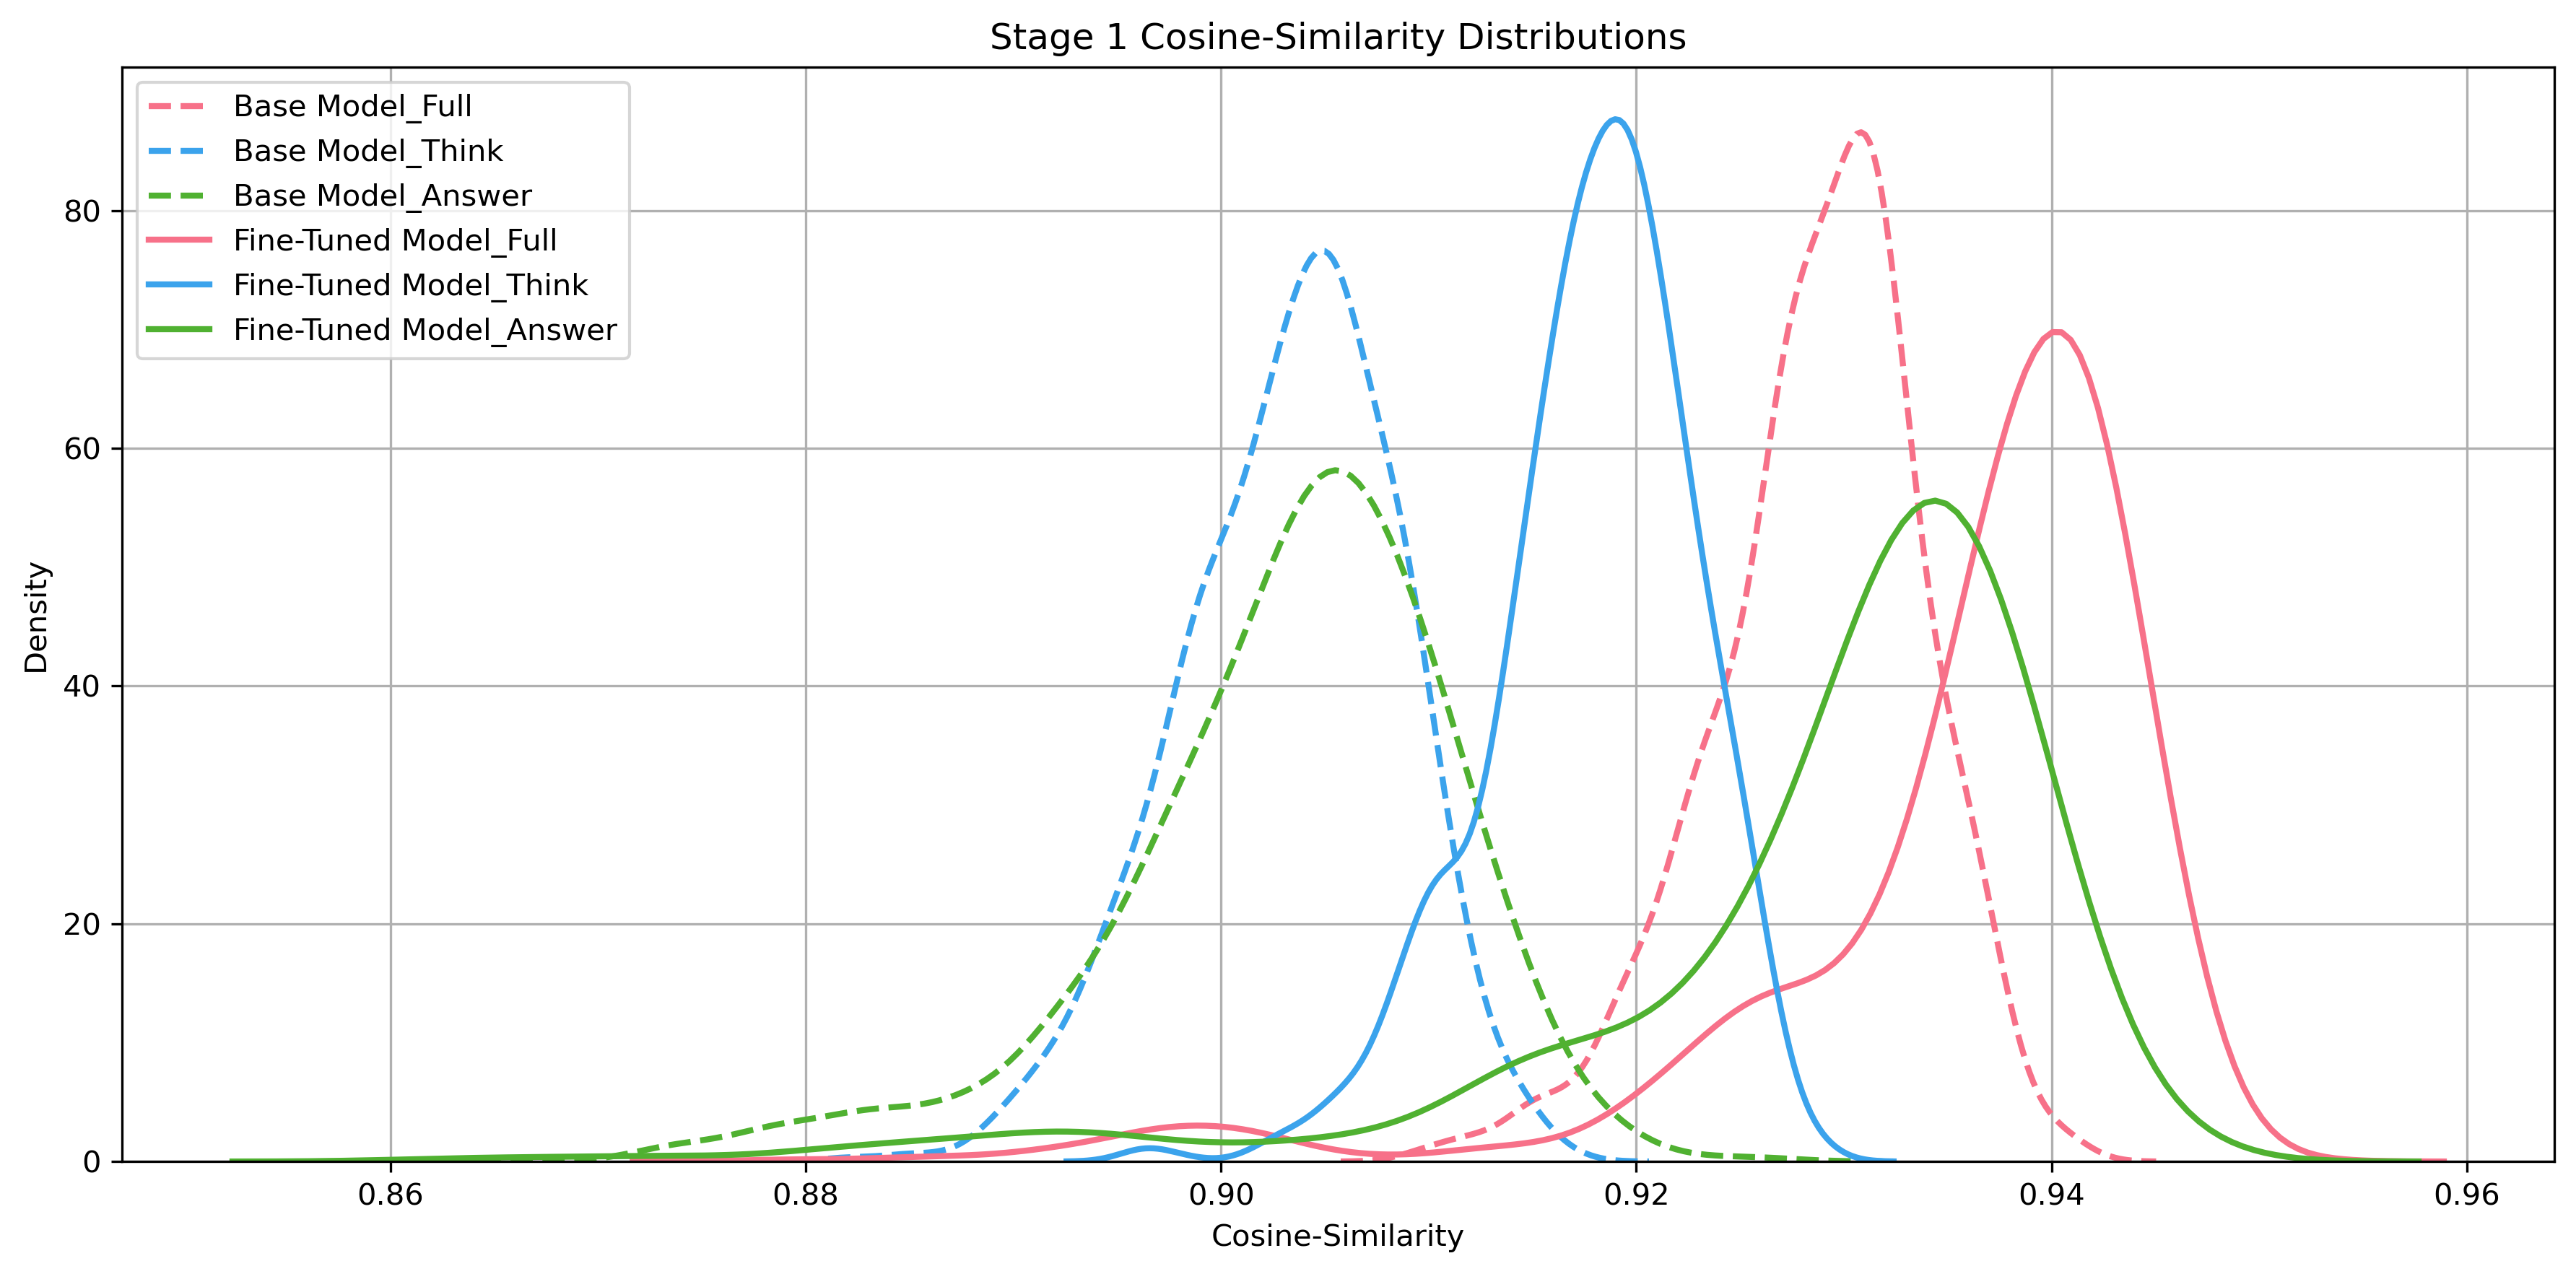
\includegraphics[width=\linewidth]{stage1_eval_figures/Cosine-Similarity_distribution.png}
%         \caption{Overall Training Results for Cosine-Similarity}
%         \label{fig:ch2:stage1-cos}
%     \end{minipage}
%     \hfill
%     \begin{minipage}[t]{0.48\textwidth}
%         \centering
%         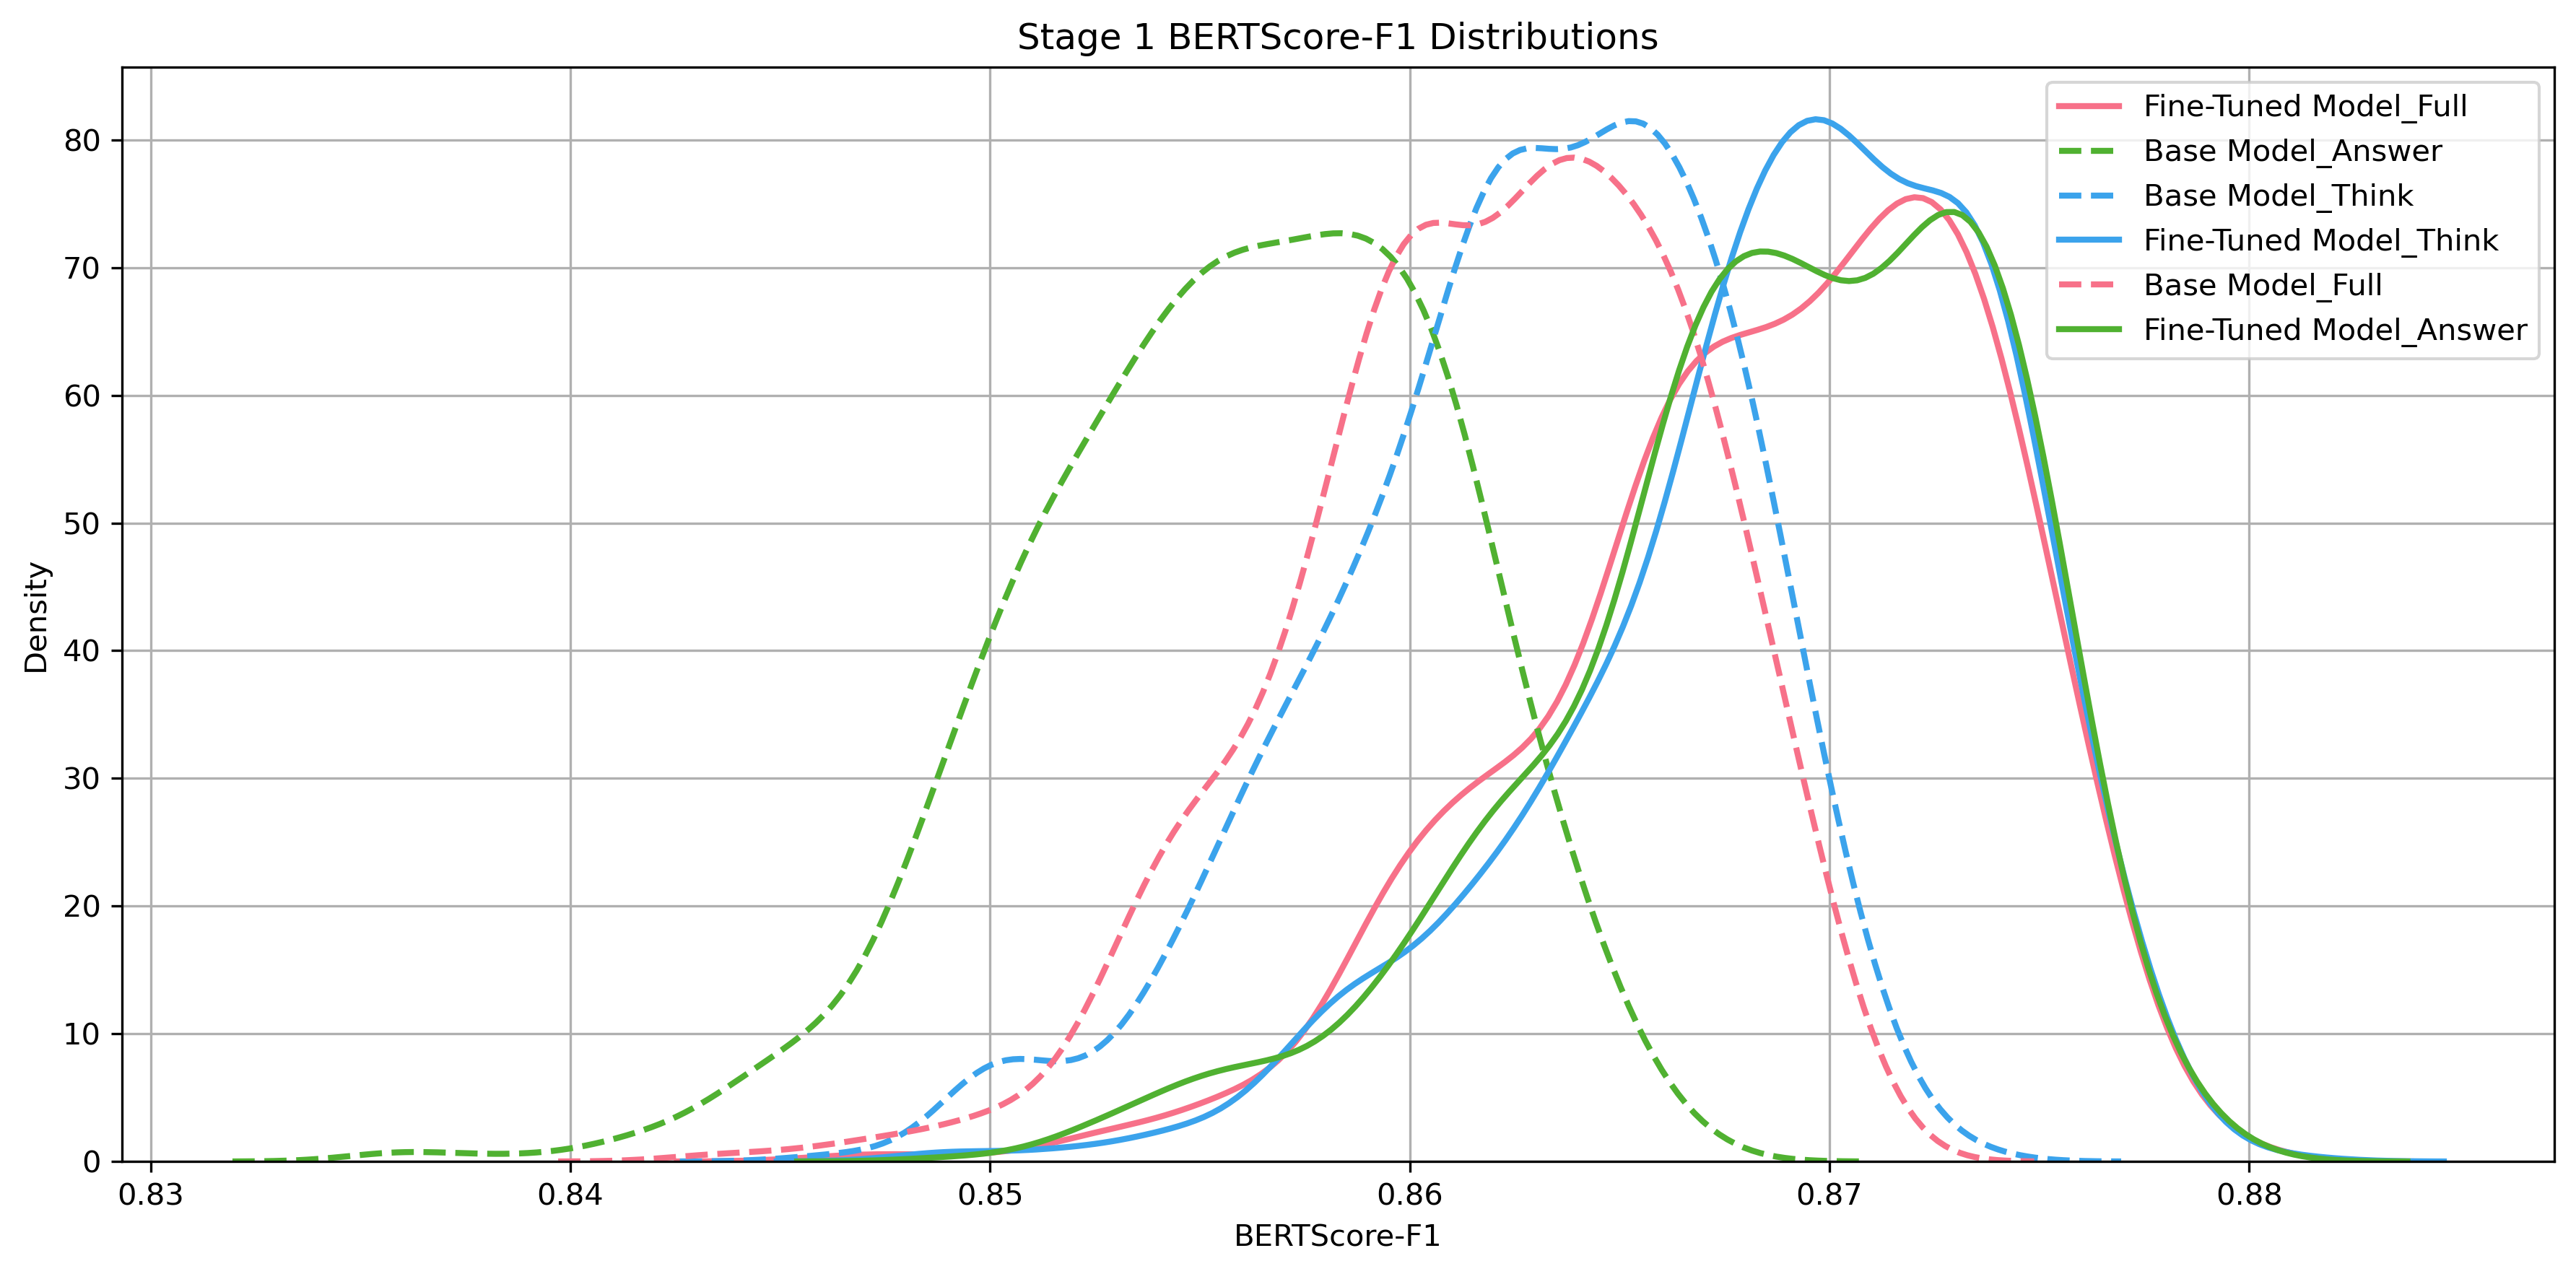
\includegraphics[width=\linewidth]{stage1_eval_figures/BERTScore-F1_distribution.png}
%         \caption{Overall Training Results for BertScore-F1}
%         \label{fig:ch2:stage1-f1}
%     \end{minipage}
% \end{figure}

% \begin{figure}[htp]
%     \centering
%     \begin{minipage}[t]{0.48\textwidth}
%         \centering
%         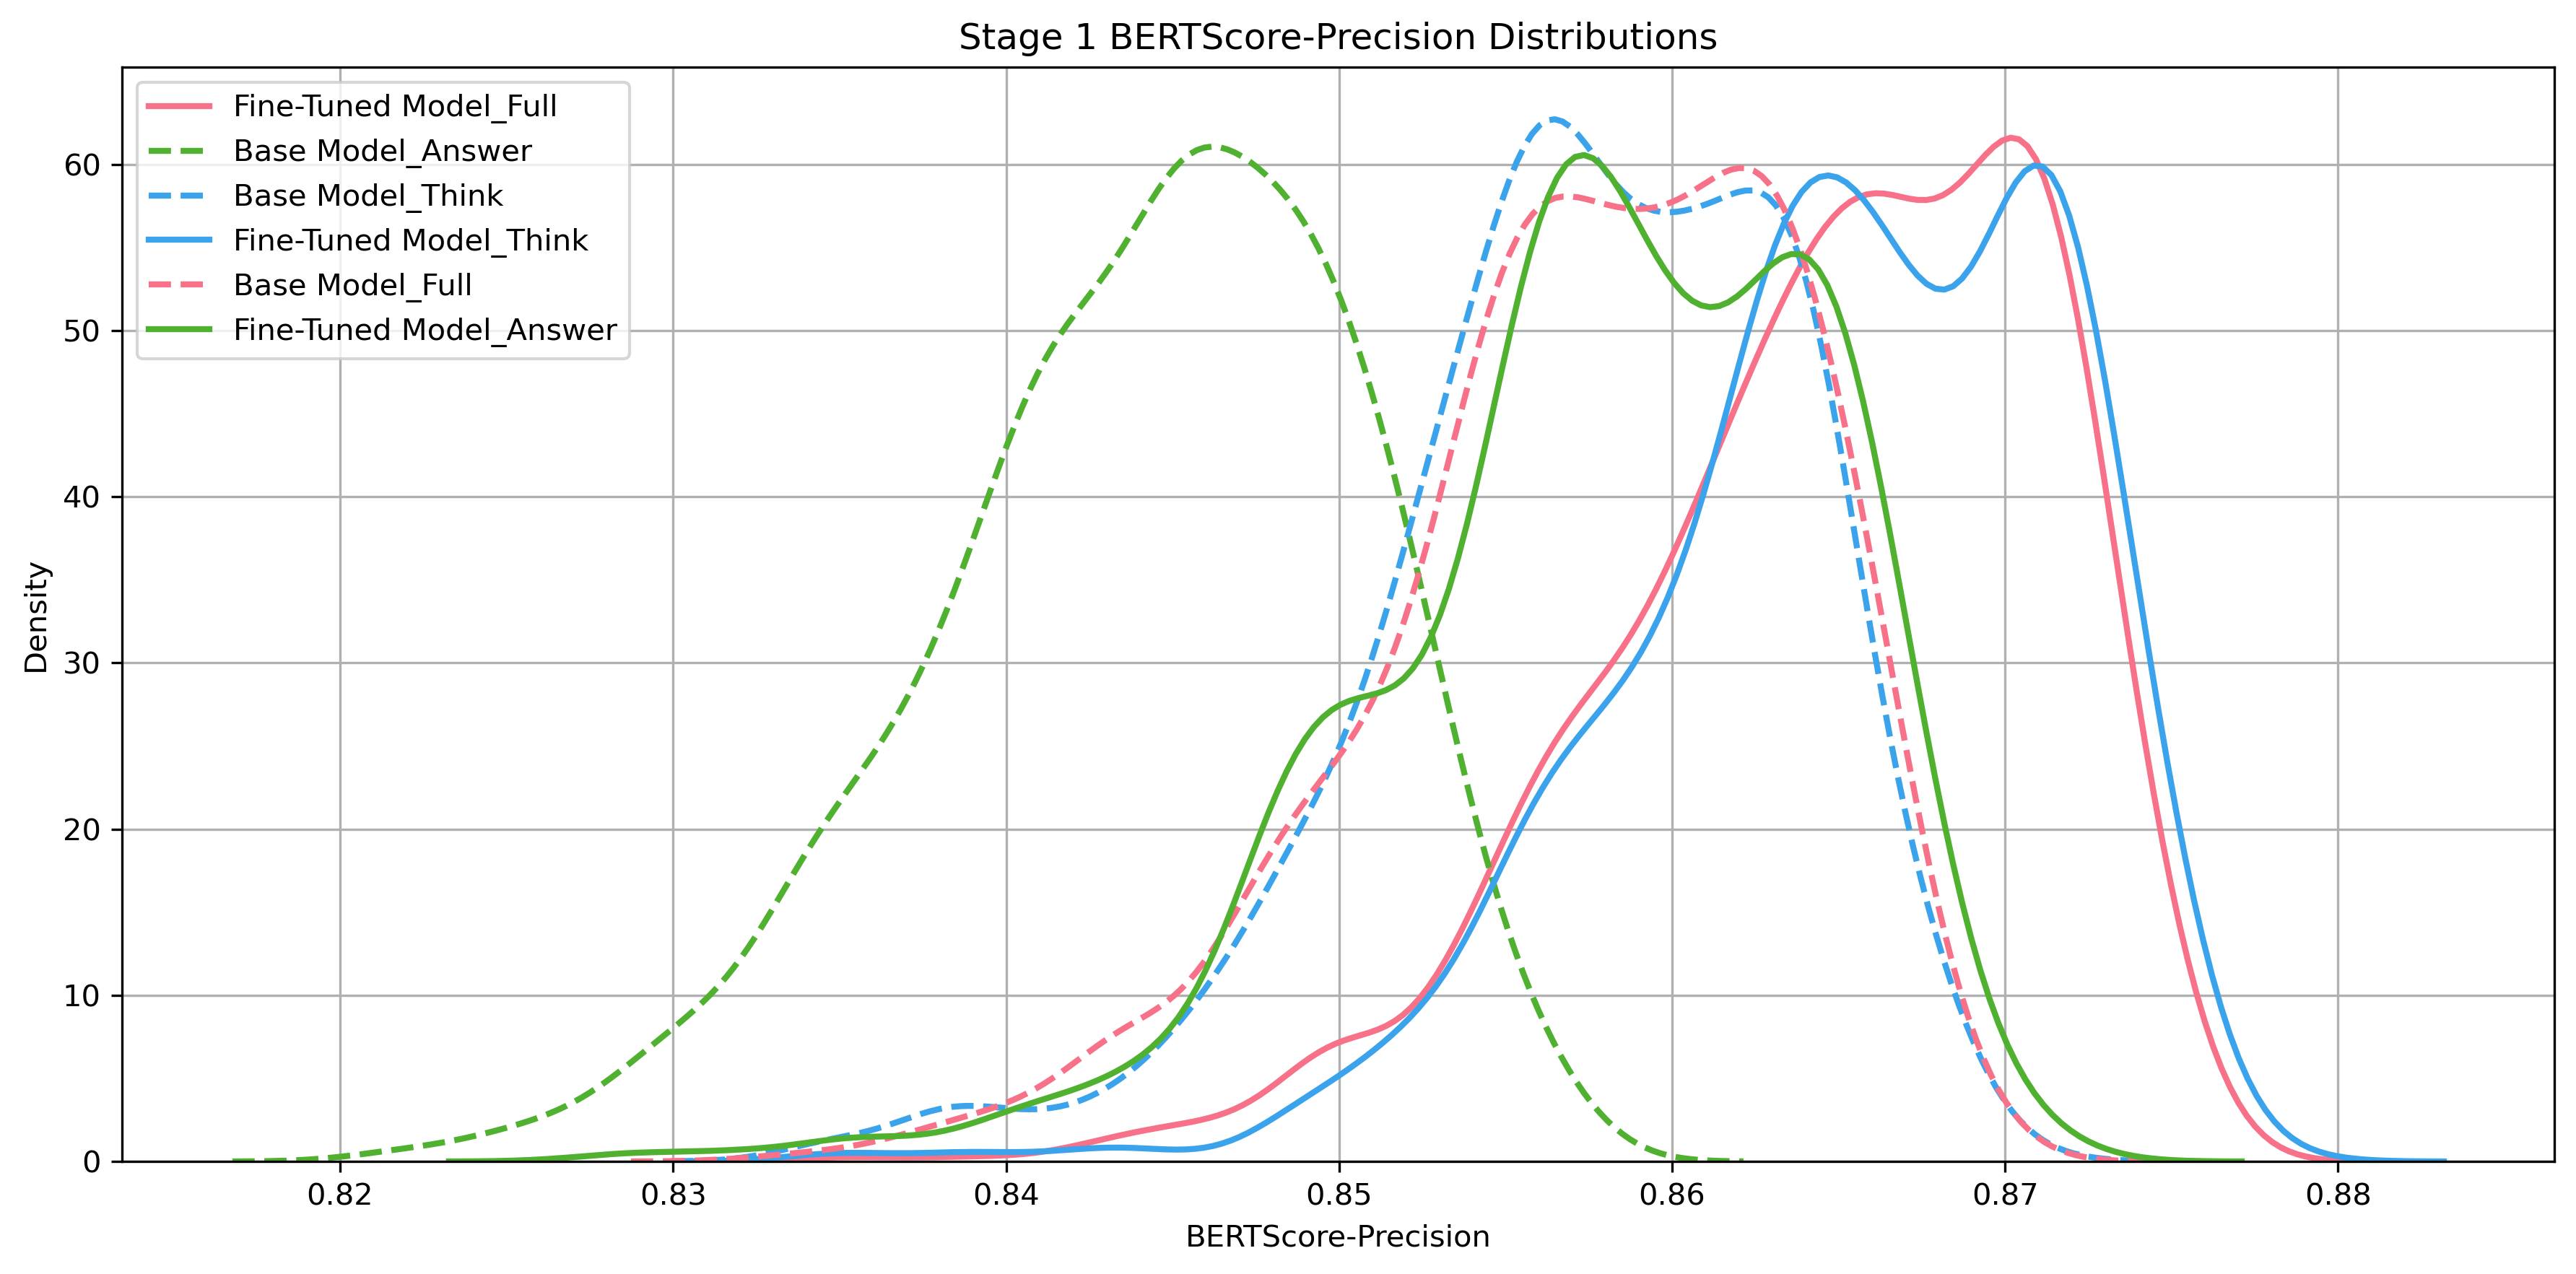
\includegraphics[width=\linewidth]{stage1_eval_figures/BERTScore-Precision_distribution.png}
%         \caption{Overall Training Results for BertScore-Precision}
%         \label{fig:ch2:stage1-precision}
%     \end{minipage}
%     \hfill
%     \begin{minipage}[t]{0.48\textwidth}
%         \centering
%         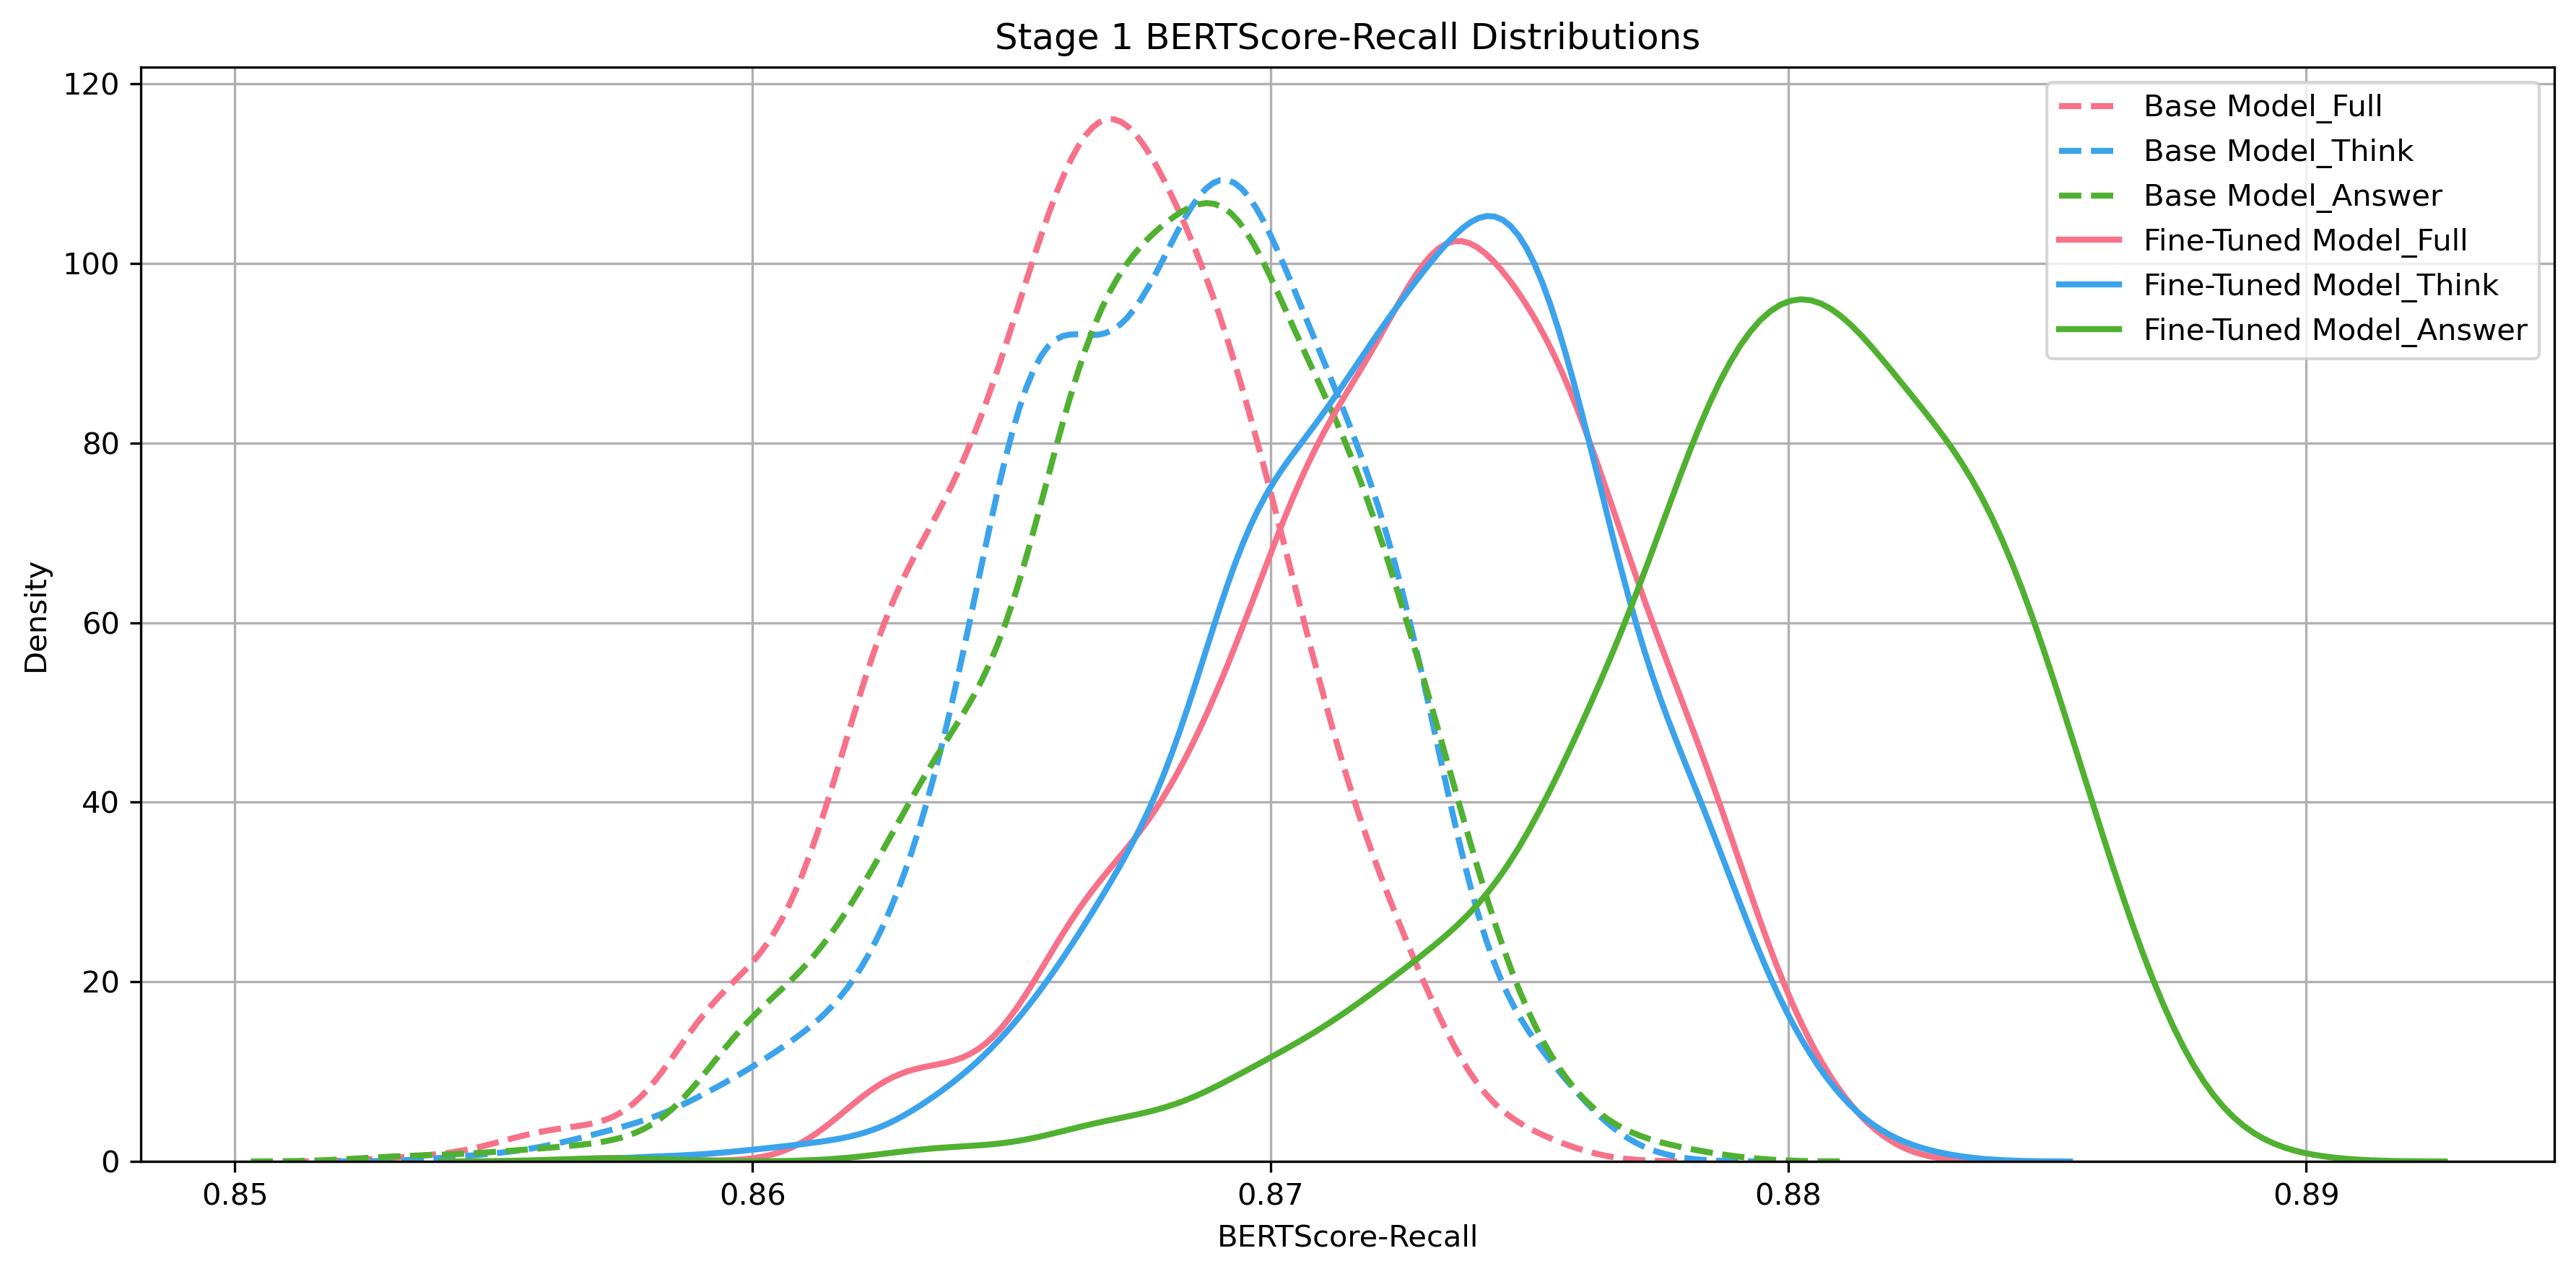
\includegraphics[width=\linewidth]{stage1_eval_figures/BERTScore-Recall_distribution.png}
%         \caption{Overall Training Results for BertScore-Recall}
%         \label{fig:ch2:stage1-recall}
%     \end{minipage}
% \end{figure}


% \begin{table}[htp]
%     \centering
%     \footnotesize
%     \begin{tabular}{l c c c}
%         \toprule
%                     & Fine-Tuned Model&     Base Model& Difference (in \%)\\
%         \hline
%         $Cos_{full}$&           0.9357&         0.9287& 0.7575 \\
%                     &  $({2912.33}^{***})$&$({5742.71}^{***})$& $({19.45}^{***})$ \\
%         $Cos_{think}$& 0.9178&0.9033&1.617 \\
%                     &$({5898.69}^{***})$&$({5396.43}^{***})$&$({62.87}^{***})$ \\
%         $Cos_{answer}$&0.929&0.9031&2.872 \\
%                     &$({2365.92}^{***})$&$({3488.41}^{***})$&$({53.63}^{***})$ \\
%         \hline
%         $BertScore_{full}^{Precision}$&0.8647&0.8575&0.8441 \\
%                     &$({4224.71}^{***})$&$({4297.97}^{***})$&$({25.10}^{***})$ \\
%         $BertScore_{think}^{Precision}$&0.8653&0.8574&0.917 \\
%                     &$({4266.65}^{***})$&$({4402.03}^{***})$&$({28.16}^{***})$ \\
%         $BertScore_{answer}^{Precision}$& 0.8579& 0.8441& 1.6387\\
%                     &$({4049.85}^{***})$&$({4181.28}^{***})$&$({47.84}^{***})$ \\

%         \hline
%         $BertScore_{full}^{Recall}$&0.8728&0.8664&0.7372 \\
%                     &$({7081.24}^{***})$&$({7889.06}^{***})$&$({37.86}^{***})$ \\
%         $BertScore_{think}^{Recall}$&0.8728&0.8681&0.5398 \\
%                     &$({7361.39}^{***})$&$({7787.30}^{***})$&$({28.21}^{***})$ \\
%         $BertScore_{answer}^{Recall}$&0.8796&0.868&1.3372 \\
%                     &$({6304.12}^{***})$&$({7364.94}^{***})$&$({63.64}^{***})$ \\

%         \hline
%         $BertScore_{full}^{F1}$&0.8686&0.862&0.7673\\
%                     &$({5207.58}^{***})$&$({5842.11}^{***})$&$({29.61}^{***})$ \\
%         $BertScore_{think}^{F1}$&0.8691&0.8628&0.7350\\
%                     &$({5509.68}^{***})$&$({5800.15}^{***})$&$({29.43}^{***})$\\
%         $BertScore_{answer}^{F1}$&0.8688&0.8558&1.5207 \\
%                     &$({5245.30}^{***})$&$({5465.88}^{***})$&$({57.07}^{***})$ \\
%         \bottomrule
%     \end{tabular}
%     \caption{Summary Overall Training Results for Cosine Similarity and BertScore tests}
%     \label{tab:ch2:result_cos}
% \end{table}



% %%% end of overall performance


\subsubsection*{Textual Similarity Performance}

% To assess the effectiveness of the fine-tuned model compared to the base model, we measured performance across sentence-level Cosine Similarity and token-level BertScore metrics.  We conduct the both tests for all three parts: the full generated text, the reasoning process ($c_i$, marked as ``think''), and the final answer ($a_i$, marked as ``answer'').
%
% Table~\ref{tab:ch2:result_cos_stage2_synthetic} illustrated the test result for the Fine-tuned Model and the Base Model (the model from Stage 1). Figure~\ref{fig:ch2:stage2-cos} illustrates the distribution of Cosine Similarity scores. Figures~\ref{fig:ch2:stage2-f1}, \ref{fig:ch2:stage2-precision}, and \ref{fig:ch2:stage2-recall} display the BERTScore results for this stage in terms of F1 Score, Precision, and Recall, respectively. As our target is to generate synthetic FOMC minutes,  the ``answer'' part is our priority focus. 
% [Codex 修改版] 2026-02-26: 消除“Stage 1/Stage 2”在不同任务间的混用，明确对比对象为“Minutes 对齐模型 vs. 领域适配基线”。
To assess the effectiveness of Minutes-style alignment, we evaluate performance using sentence-level Cosine Similarity and token-level BERTScore. We report results for (i) the full generated text, (ii) the reasoning trajectory ($c_i$, marked as ``think''), and (iii) the final answer ($a_i$, marked as ``answer'').

% [CH2-125][Original Start]
% Table~\ref{tab:ch2:result_cos_stage2_synthetic} compares the Minutes-aligned fine-tuned model against the domain-adapted baseline model (trained via the two-step SFT+GRPO pipeline). Figure~\ref{fig:ch2:stage2-cos} shows the distribution of Cosine Similarity scores, while Figures~\ref{fig:ch2:stage2-f1}, \ref{fig:ch2:stage2-precision}, and \ref{fig:ch2:stage2-recall} report BERTScore in terms of F1, Precision, and Recall. Since the primary objective is synthetic Minutes generation, we focus on the ``answer'' segment.
% [CH2-125][Original End]
Table~\ref{tab:ch2:result_cos_stage2_synthetic} compares Checkpoint-3 (Minutes-style alignment) against Checkpoint-2 (analysis GRPO). Figure~\ref{fig:ch2:stage2-cos} shows the distribution of Cosine Similarity scores, while Figures~\ref{fig:ch2:stage2-f1}, \ref{fig:ch2:stage2-precision}, and \ref{fig:ch2:stage2-recall} report BERTScore in terms of F1, Precision, and Recall. Since the primary objective is synthetic Minutes generation, we focus on the ``answer'' segment.

% [CH2-089][Original Start]
% Noticeably, the results from all evaluation metrics confirmed the improvements of the fine-tuning. The percentage changes in all metrics of the ``answer'' part is significantly higher than the other parts. For instance, the $Cos$ difference for the ``answer'' is 2.872\% while only 0.7575\% for the ``full'' response. The $BertScore_{answer}^{F1}$ difference is 1.5207\% which is twice higher than the $BertScore_{full}^{f1}$ (0.7673\%). Both results are statistically significant at 0.1\% level.
% [CH2-089][Original End]
% [CH2-110][Original Start]
% All reported metrics improve after fine-tuning, with the largest gains in the ``answer'' segment. For example, the cosine-similarity gain is 2.872\% for ``answer'' versus 0.7575\% for ``full'' text. The gain in $BertScore_{answer}^{F1}$ is 1.5207\%, roughly twice the $BertScore_{full}^{F1}$ gain (0.7673\%). These differences are statistically significant at the 0.1\% level.
% [CH2-110][Original End]
% [CH2-126][Original Start]
% All reported metrics improve after fine-tuning, with the largest gains in the ``answer'' segment. For example, the cosine-similarity gain is 2.872\% for ``answer'' versus 0.7575\% for ``full'' text. The gain in $BERTScore_{answer}^{F1}$ is 1.5207\%, roughly twice the $BERTScore_{full}^{F1}$ gain (0.7673\%). These differences are statistically significant at the 0.1\% level.
% [CH2-126][Original End]
All reported metrics improve for Checkpoint-3 relative to Checkpoint-2, with the largest gains in the ``answer'' segment. For example, the cosine-similarity gain is 2.872\% for ``answer'' versus 0.7575\% for ``full'' text. The gain in $BERTScore_{answer}^{F1}$ is 1.5207\%, roughly twice the $BERTScore_{full}^{F1}$ gain (0.7673\%). These differences are statistically significant on the held-out alignment split used for the reported comparison.



\begin{figure}[htp]
    \centering
    \begin{minipage}[t]{0.48\textwidth}
        \centering
        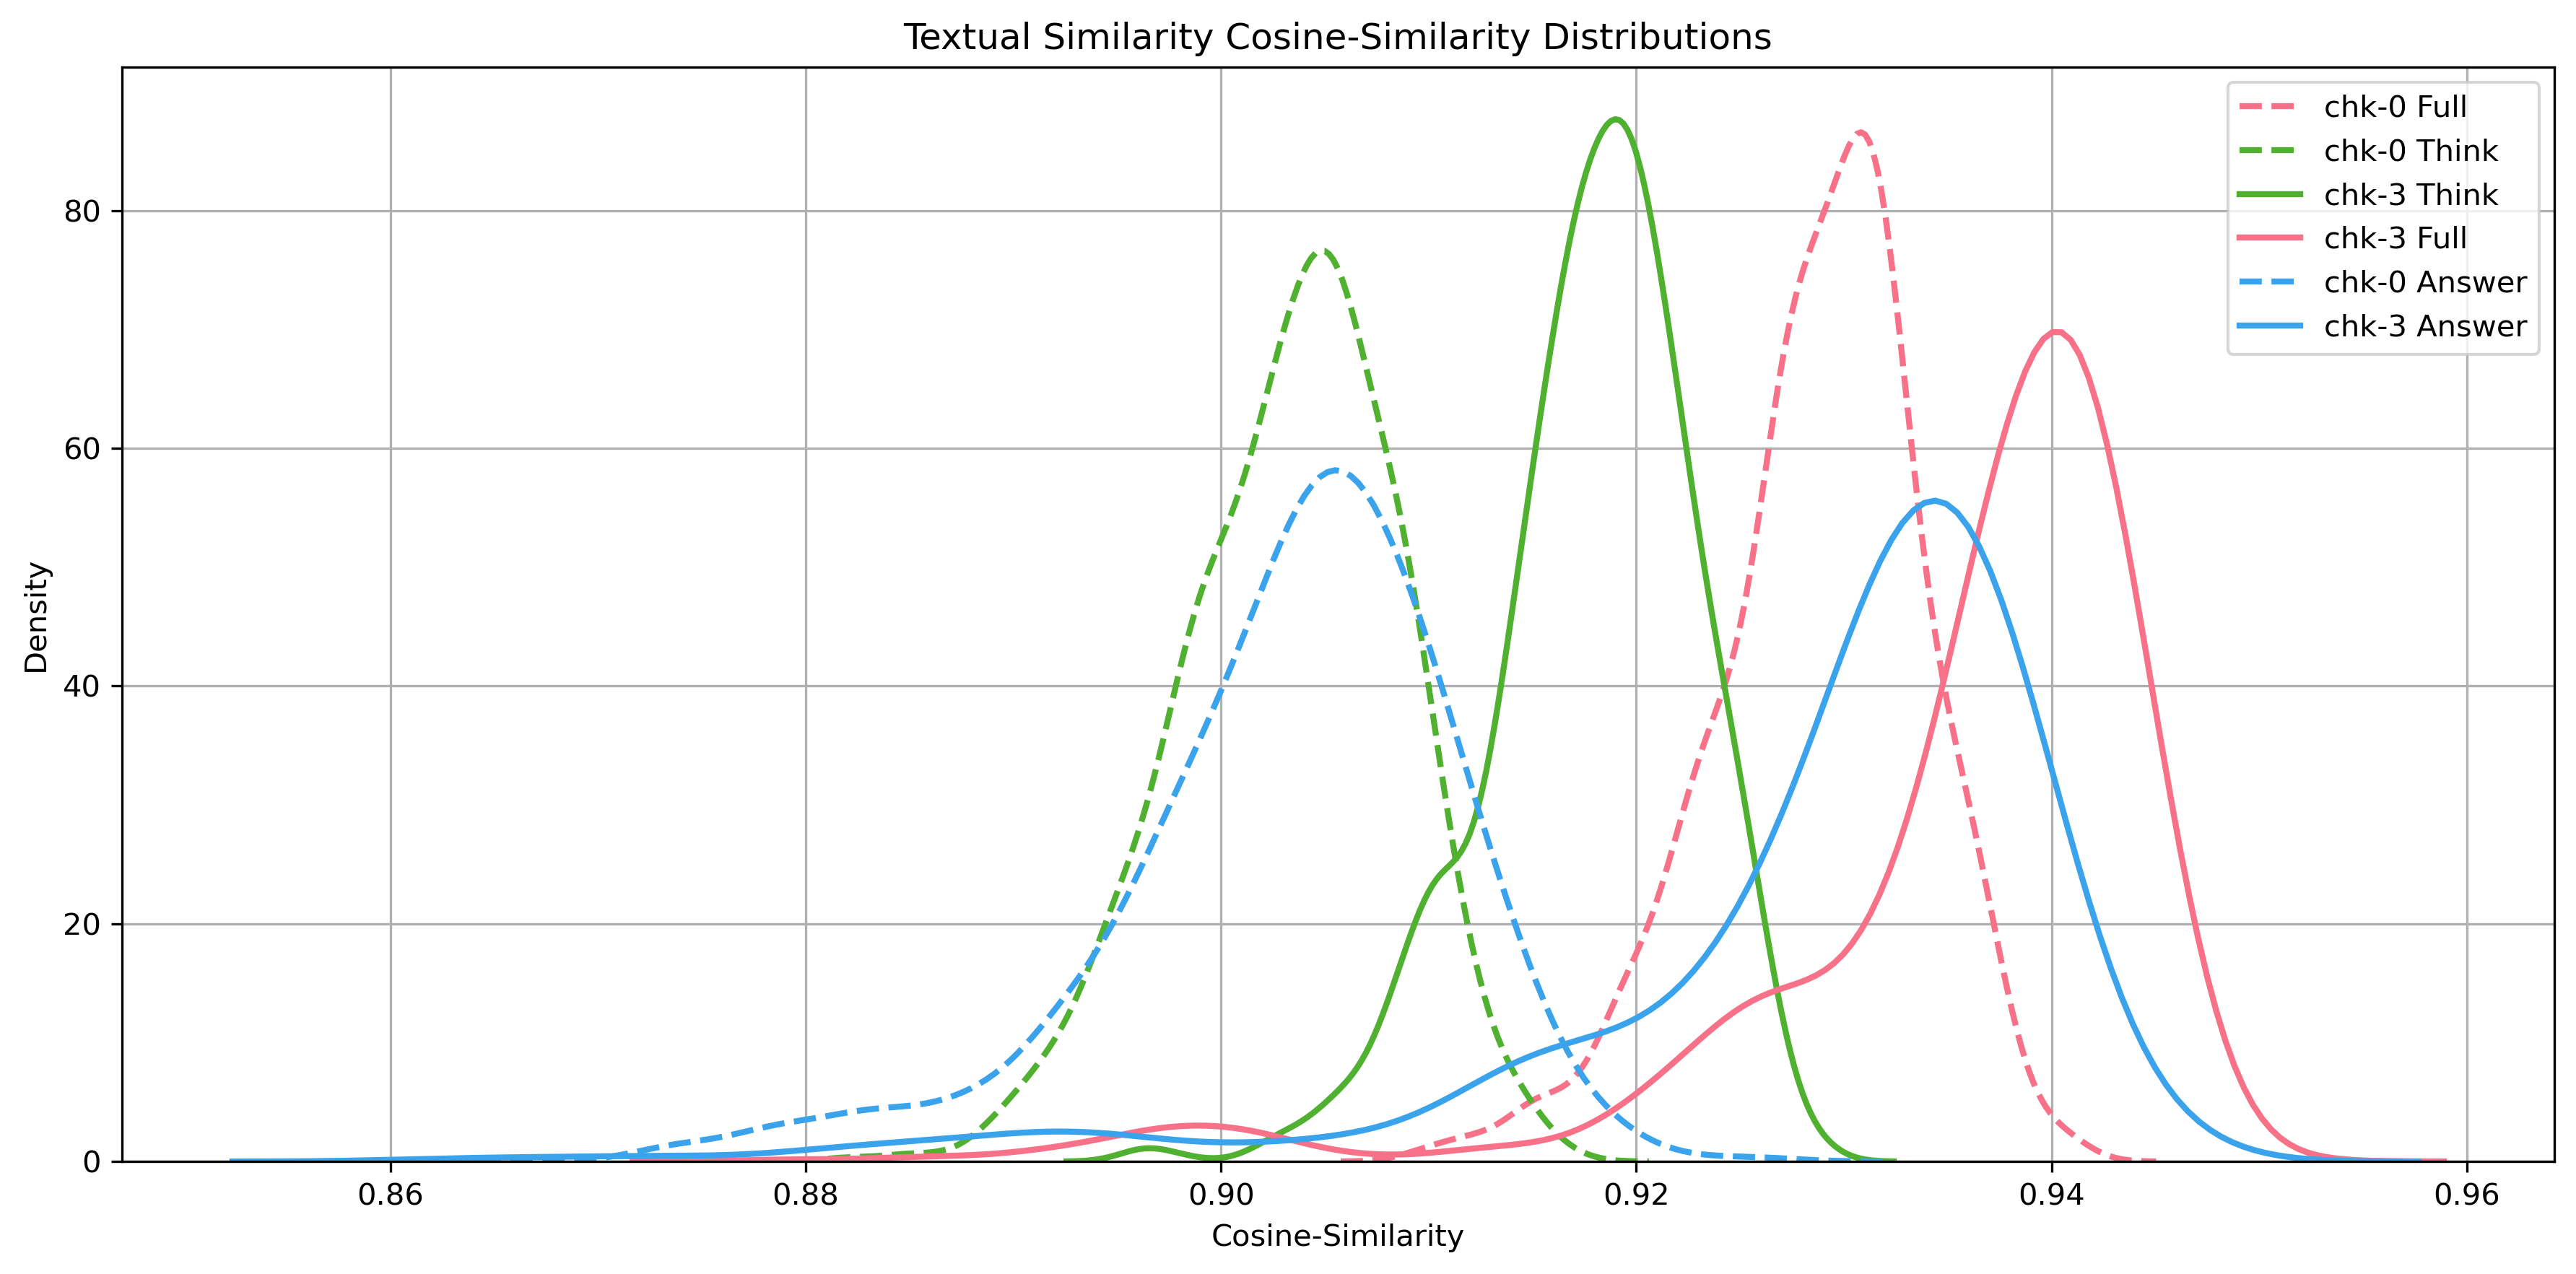
\includegraphics[width=\linewidth]{stage2_eval_figures/stage2_Cosine-Similarity_distribution.png}
        \caption{Textual Similarity Result for Cosine-Similarity}
        \label{fig:ch2:stage2-cos}
    \end{minipage}
    \hfill
    \begin{minipage}[t]{0.48\textwidth}
        \centering
        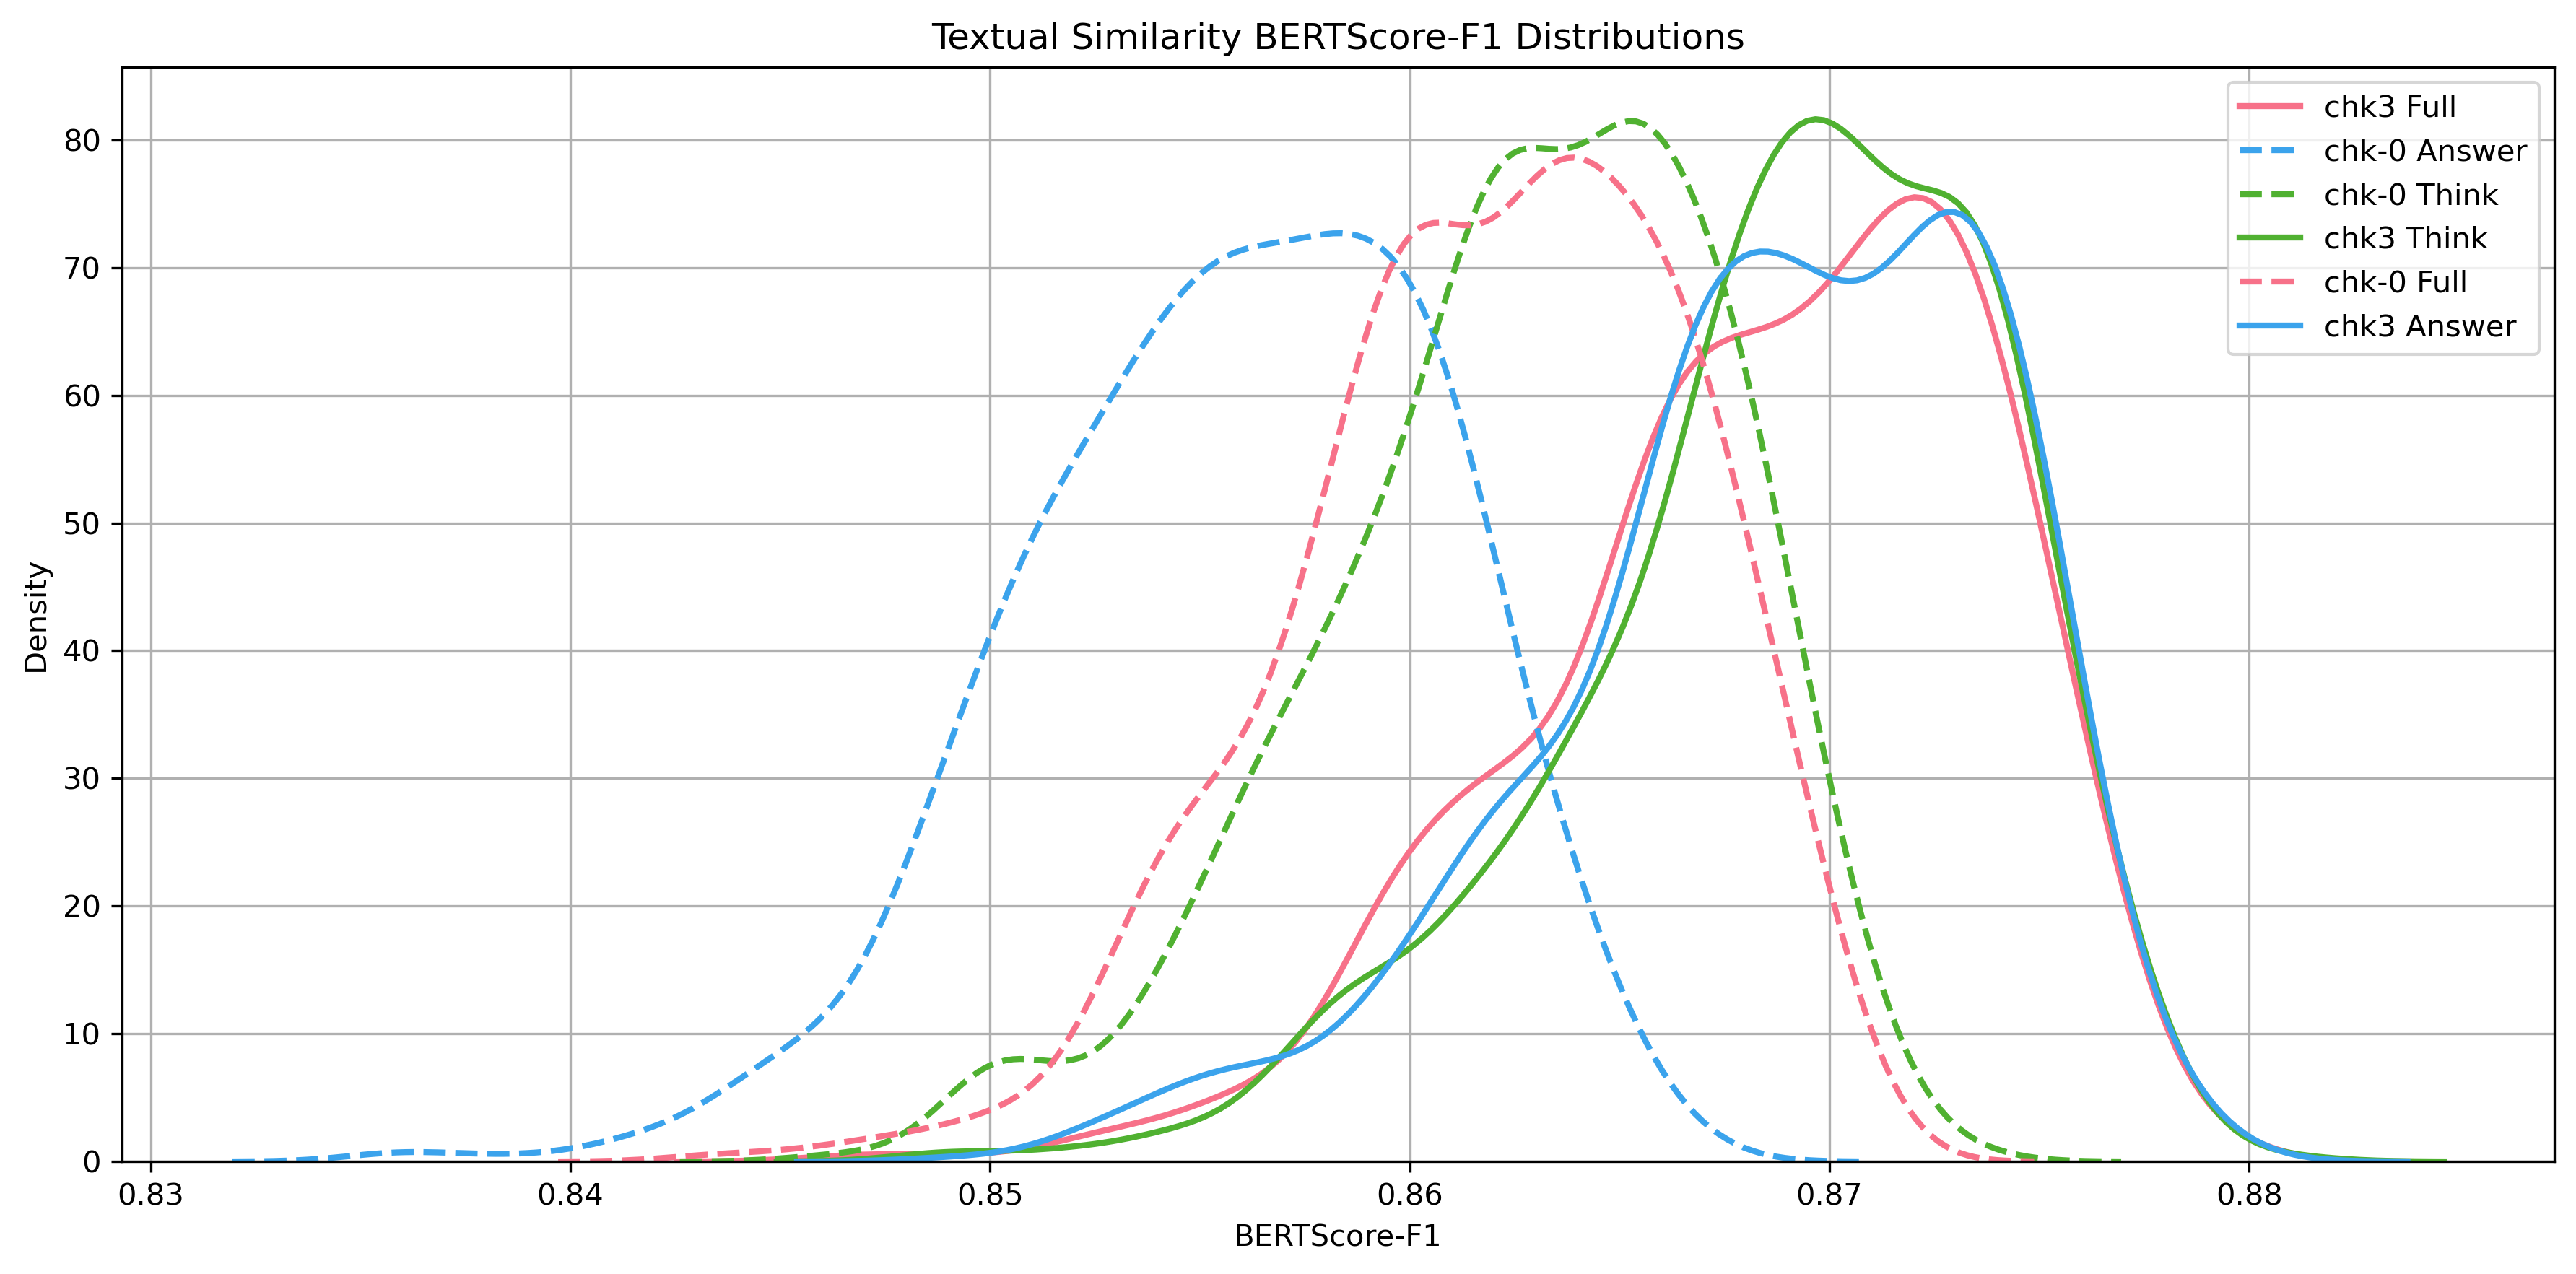
\includegraphics[width=\linewidth]{stage2_eval_figures/stage2_BERTScore-F1_distribution.png}
        \caption{Textual Similarity Result for BERTScore-F1}
        \label{fig:ch2:stage2-f1}
    \end{minipage}
\end{figure}

\begin{figure}[htp]
    \centering
    \begin{minipage}[t]{0.48\textwidth}
        \centering
        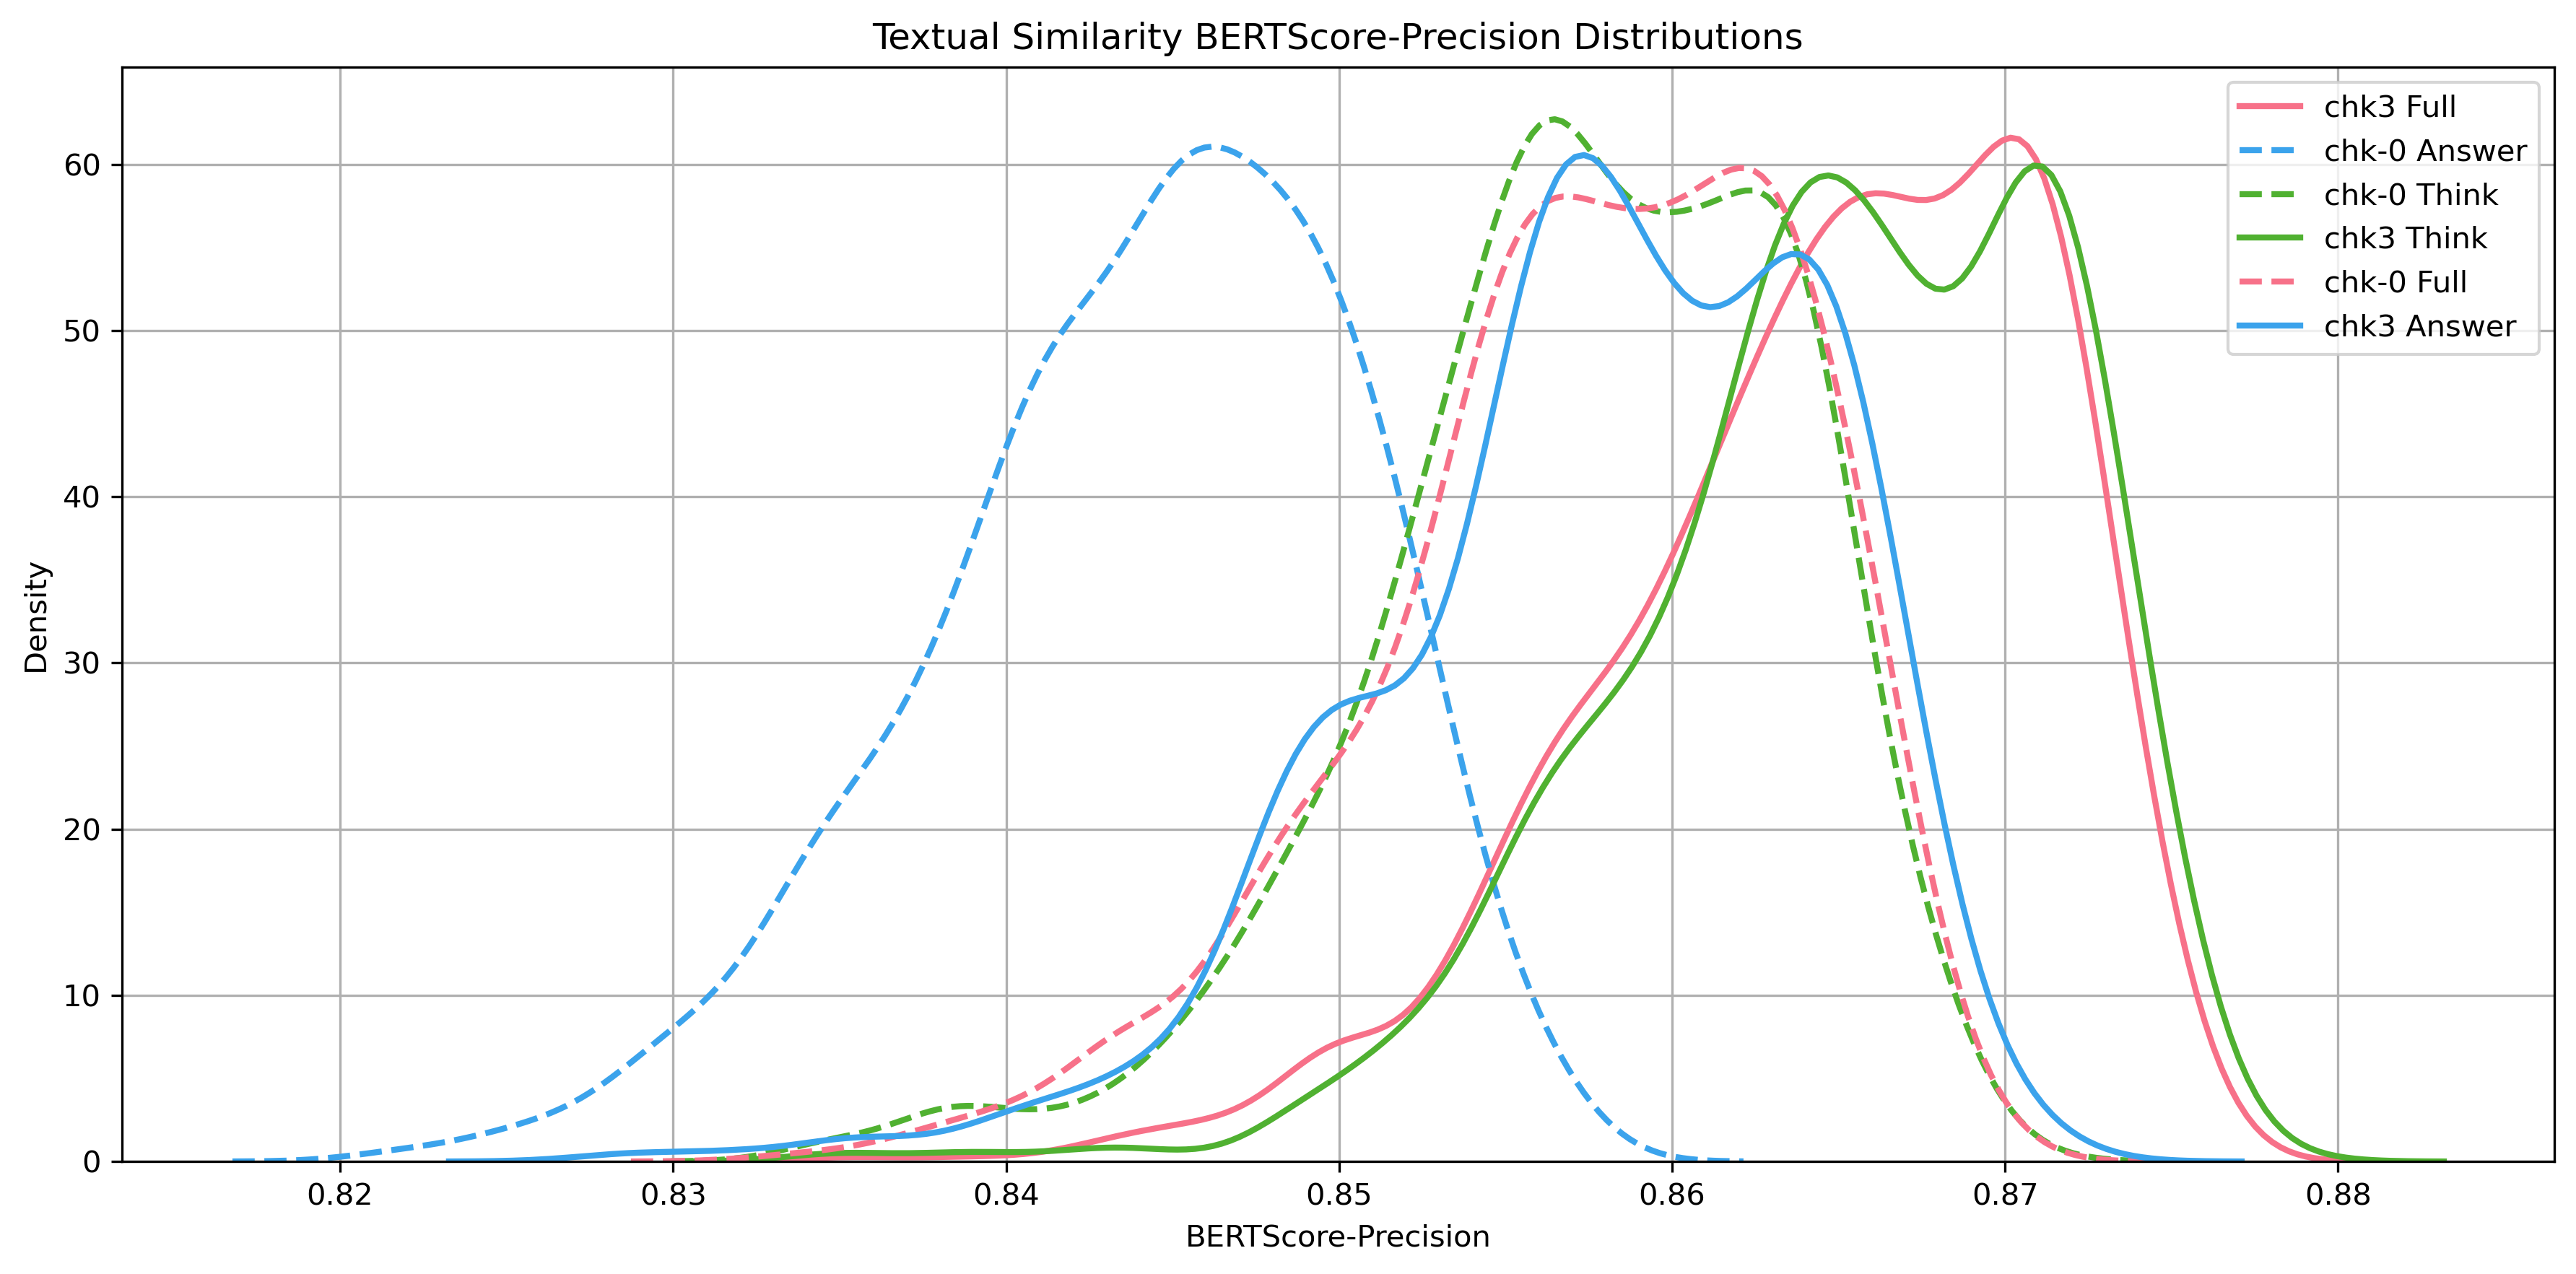
\includegraphics[width=\linewidth]{stage2_eval_figures/stage2_BERTScore-Precision_distribution.png}
        \caption{Textual Similarity Result for BERTScore-Precision}
        \label{fig:ch2:stage2-precision}
    \end{minipage}
    \hfill
    \begin{minipage}[t]{0.48\textwidth}
        \centering
        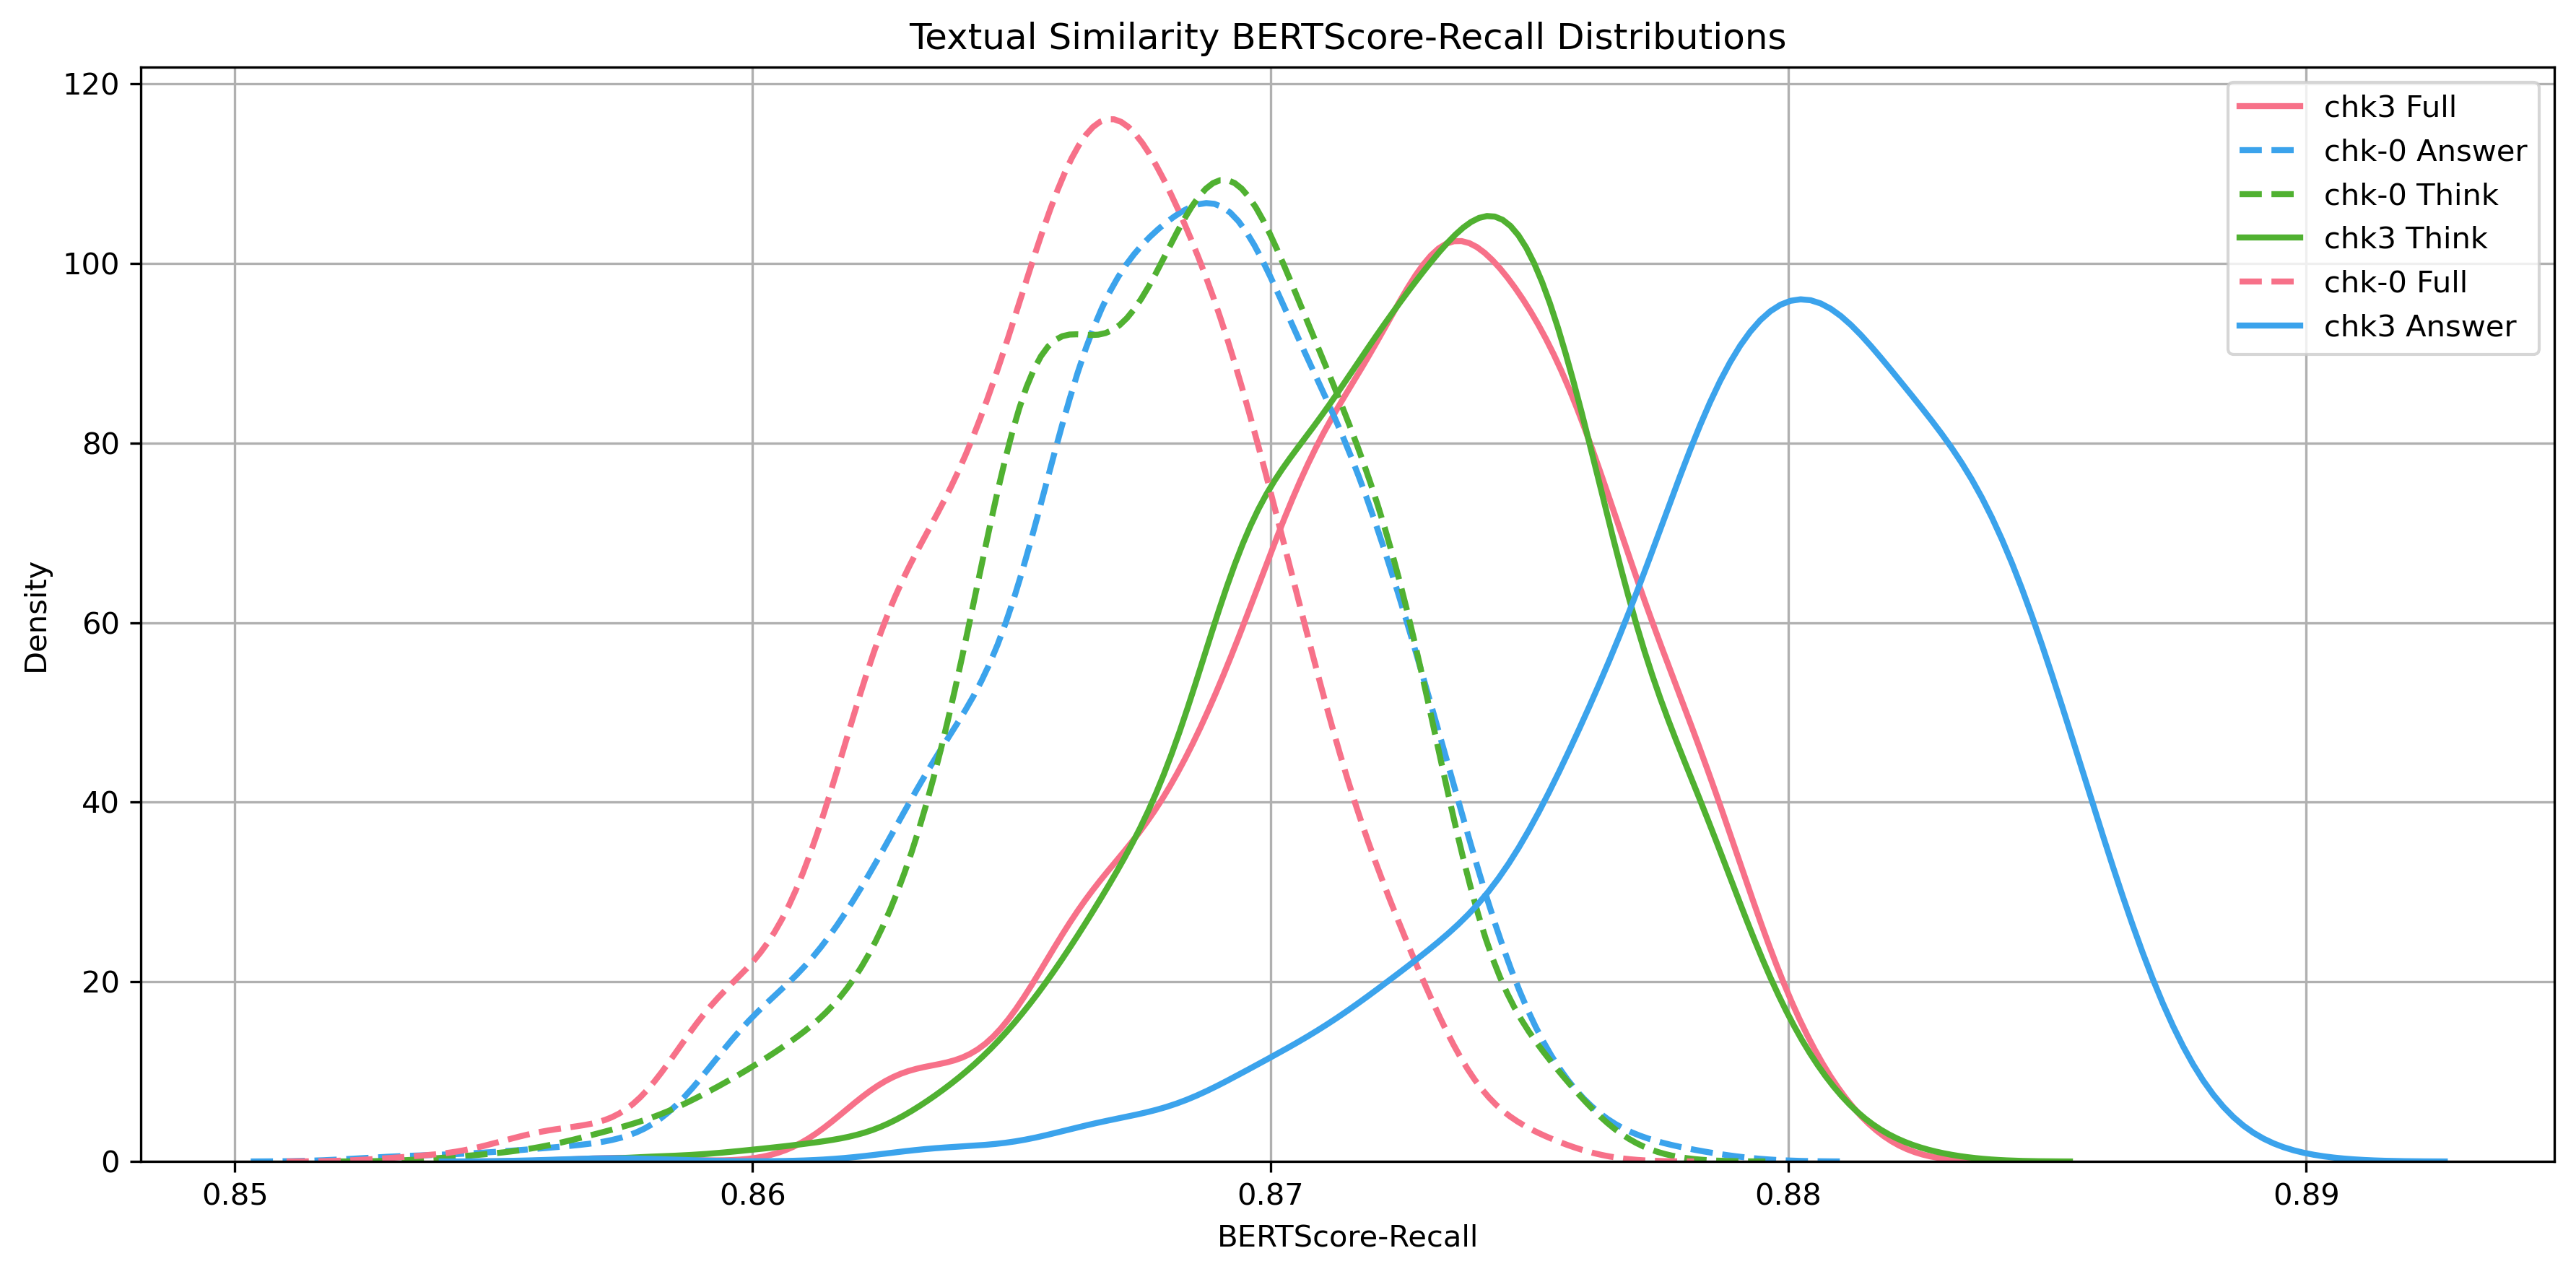
\includegraphics[width=\linewidth]{stage2_eval_figures/stage2_BERTScore-Recall_distribution.png}
        \caption{Textual Similarity Result for BERTScore-Recall}
        \label{fig:ch2:stage2-recall}
    \end{minipage}
\end{figure}






\begin{table}[htp]
    \centering
    \footnotesize
    \begin{tabular}{l c c c}
        \toprule
        & Checkpoint-3&     Checkpoint-2& Difference (in \%)\\
        \hline
        $Cos_{full}$&0.9357&0.9287&0.7575\\ 
                    &$({2912.33}^{***})$&$({5742.71}^{***})$&$({19.49}^{***})$\\ 
        $Cos_{think}$&0.9178&0.9033&1.617\\ 
                    &$({5898.69}^{***})$&$({5396.43}^{***})$&$({62.87}^{***})$\\ 
        $Cos_{answer}$&0.929&0.9031&\textbf{2.872}\\ 
                    &$({2365.92}^{***})$&$({3488.41}^{***})$&$({53.63}^{***})$\\
        \hline
        % [CH2-111][Original Start]
        % $BertScore_{full}^{Precision}$&0.8647&0.8575&0.8441\\ 
        %             &$({4224.71}^{***})$&$({4297.97}^{***})$&$({25.10}^{***})$\\ 
        % $BertScore_{think}^{Precision}$&0.8653&0.8574&0.917\\ 
        %             &$({4266.65}^{***})$&$({4402.03}^{***})$&$({28.16}^{***})$\\ 
        % $BertScore_{answer}^{Precision}$&0.8579&0.8441&\textbf{1.6387}\\ 
        %             &$({4049.85}^{***})$&$({4181.28}^{***})$&$({47.84}^{***})$\\ 
        %
        % \hline
        % $BertScore_{full}^{Recall}$&0.8728&0.8664&0.7372\\ 
        %             &$({7081.24}^{***})$&$({7889.06}^{***})$&$({37.86}^{***})$\\ 
        % $BertScore_{think}^{Recall}$&0.8728&0.8681&0.5398\\ 
        %             &$({7361.39}^{***})$&$({7787.30}^{***})$&$({28.21}^{***})$\\ 
        % $BertScore_{answer}^{Recall}$&0.8796&0.868&\textbf{1.3372}\\ 
        %             &$({6304.12}^{***})$&$({7364.94}^{***})$&$({63.64}^{***})$\\ 
        %
        % \hline
        % $BertScore_{full}^{F1}$&0.8686&0.862&0.7673\\ 
        %             &$({5207.58}^{***})$&$({5842.11}^{***})$&$({29.61}^{***})$\\ 
        % $BertScore_{think}^{F1}$&0.8691&0.8628&0.735\\ 
        %             &$({5509.68}^{***})$&$({5800.15}^{***})$&$({29.43}^{***})$\\ 
        % $BertScore_{answer}^{F1}$&0.8688&0.8558&1.5207\\ 
        %             &$({5245.30}^{***})$&$({5465.88}^{***})$&$({57.07}^{***})$\\ 
        % [CH2-111][Original End]
        $BERTScore_{full}^{Precision}$&0.8647&0.8575&0.8441\\ 
                    &$({4224.71}^{***})$&$({4297.97}^{***})$&$({25.10}^{***})$\\ 
        $BERTScore_{think}^{Precision}$&0.8653&0.8574&0.917\\ 
                    &$({4266.65}^{***})$&$({4402.03}^{***})$&$({28.16}^{***})$\\ 
        $BERTScore_{answer}^{Precision}$&0.8579&0.8441&\textbf{1.6387}\\ 
                    &$({4049.85}^{***})$&$({4181.28}^{***})$&$({47.84}^{***})$\\ 

        \hline
        $BERTScore_{full}^{Recall}$&0.8728&0.8664&0.7372\\ 
                    &$({7081.24}^{***})$&$({7889.06}^{***})$&$({37.86}^{***})$\\ 
        $BERTScore_{think}^{Recall}$&0.8728&0.8681&0.5398\\ 
                    &$({7361.39}^{***})$&$({7787.30}^{***})$&$({28.21}^{***})$\\ 
        $BERTScore_{answer}^{Recall}$&0.8796&0.868&\textbf{1.3372}\\ 
                    &$({6304.12}^{***})$&$({7364.94}^{***})$&$({63.64}^{***})$\\ 

        \hline
        $BERTScore_{full}^{F1}$&0.8686&0.862&0.7673\\ 
                    &$({5207.58}^{***})$&$({5842.11}^{***})$&$({29.61}^{***})$\\ 
        $BERTScore_{think}^{F1}$&0.8691&0.8628&0.735\\ 
                    &$({5509.68}^{***})$&$({5800.15}^{***})$&$({29.43}^{***})$\\ 
        $BERTScore_{answer}^{F1}$&0.8688&0.8558&1.5207\\ 
                    &$({5245.30}^{***})$&$({5465.88}^{***})$&$({57.07}^{***})$\\ 
        \bottomrule
    \end{tabular}
    \caption{Summary Textual Similarity Results for Cosine Similarity and BERTScore Tests}
    \label{tab:ch2:result_cos_stage2_synthetic}
\end{table}


% [CH2-127][Original Start]
% In summary, the findings indicate that the fine-tuned model effectively captures and reproduces the linguistic style, analytical reasoning, and structural coherence of authentic FOMC Minutes, demonstrating high fidelity at both the sentence and token levels.
% [CH2-127][Original End]
In summary, the reported comparison indicates that Checkpoint-3 is closer than Checkpoint-2 to the reference Minutes on this alignment split, especially for the final answer segment. This supports the claim that the Minutes-style adaptation stage improves stylistic and semantic closeness, although the evidence should still be interpreted as random held-out meeting validation rather than as a temporal holdout.



%%%% end of textual similarity result

\subsubsection*{Input Grounding Results under Leave-one-out Masking}

% In this section, we apply the \textbf{TokenShapley} method to compute the Shapley Value (denoted as $\mathcal{SV}_i$; see Eq.~\ref{eq:ch2:shapley}) in order to evaluate whether the generated sections contain sufficient information derived from the input prompts. Two empirical tests are conducted for this purpose. In the first test, we calculate the Shapley Value by sequentially masking different indicators in the input prompts, using both the synthetic Minutes and the actual FOMC Minutes as target outputs ($o_{target}$) for comparison. In the second test, we further examine the relative percentage contribution of each indicator to specific sections by setting the unmasked input prompt as the baseline.
% [Codex 修改版] 2026-02-26: 将结果部分与前文 leave-one-out 贡献度定义保持一致，避免“TokenShapley/ Shapley”名不副实。
% In this section, we evaluate whether the generated sections contain sufficient information grounded in the input indicators using the leave-one-out masking contribution score defined in Eq.~\ref{eq:ch2:shapley}. Two tests are conducted. In the first test, we sequentially remove each indicator from the prompt and compute its contribution $\Delta_i$ using either (i) the synthetic Minutes (generated under the unmasked prompt) or (ii) the actual FOMC Minutes as the target output $o_{target}$. In the second test, we examine relative percentage differences in $\Delta_i$ across sections to assess whether the model assigns indicators to the most contextually relevant Minutes sections.
% [Codex 修改版] 2026-02-26: 第二个测试在表格中以“相似度水平/相对变化”呈现，因此用更贴近结果展示的表述。
% [CH2-128][Original Start]
% In this section, we evaluate whether the generated sections contain sufficient information grounded in the input indicators using leave-one-out masking (Eq.~\ref{eq:ch2:shapley}). Two tests are conducted. In the first test, we sequentially remove each indicator from the prompt and evaluate its marginal effect on similarity to a target text (synthetic or real). In the second test, we examine relative percentage differences in similarity (under masking) across sections to assess whether indicators exhibit stronger relevance for specific Minutes sections.
% [CH2-128][Original End]
In this section, we evaluate whether the generated sections contain sufficient information grounded in the input indicators using leave-one-out masking (Eq.~\ref{eq:ch2:loo_masking}). Two tests are conducted. In the first test, we sequentially remove each indicator from the prompt and evaluate its marginal effect on similarity to a target text (synthetic or real). In the second test, we examine relative percentage differences in similarity (under masking) across sections to assess whether indicators exhibit stronger relevance for specific Minutes sections.

% [Codex 修改版] 2026-04-17: 明确结果表来自仓库中的过滤导出，但不把历史目录名当作方法名。
The detailed three-section tables below are regenerated from the filtered workbook exports preserved in the repository. These exports retain a historical directory naming convention, but in the chapter text the results are interpreted solely as leave-one-out masking outputs.


% In the first test, we begin by masking a specific indicator ($p_i$) within the prompt and instruct the model to generate the corresponding section of the FOMC Minutes. The resulting output with the masked prompt is denoted as $o(S)$. Simultaneously, we generate the same section based on the full prompt that includes the indicator $p_i$, denoted as $o(S \cup p_i)$. Cosine Similarity is then employed as the utility function ($Cos(\cdot)$) to evaluate the quality of the output, and the change in similarity before and after masking is used to measure the marginal contribution of each indicator. A statistically significant positive difference indicates that the masked indicator contributes positively to the generated section, reflecting its marginal informational value.
% [Codex 修改版] 2026-02-26
Concretely, for each indicator $p_i$, we generate the section once with the full prompt $\mathcal{P}$ and once with $p_i$ removed. We then compute $\Delta_i$ as the change in Cosine Similarity to the target text. A statistically significant positive $\Delta_i$ indicates that the indicator provides marginal informational value for generating that section.

We first use the synthetic Minutes generated from the unmasked prompt as the target output ($o_{target}$) in the Cosine calculation. Table~\ref{tab:ch2:shapley_result} reports the test results across the three main sections, evaluated using 25 key macroeconomic and financial indicators.

\begin{table}[htbp]
\centering
\scriptsize
\begin{threeparttable}
\begin{tabular}{p{3.6cm} p{4.3cm} p{3.1cm} p{3.1cm}}
\toprule
\textbf{Key Indicator} &
\textbf{Participants’ Views on Current Conditions and the Economic Outlook} &
\textbf{Staff Review of the Economic Situation} &
\textbf{Staff Review of the Financial Situation} \\
\midrule
Bank-Capital & $0.2164^{***}$ & $0.2054^{***}$ & $0.2168^{***}$ \\
Bank-Credit-to-Private-Sector & $0.2067^{***}$ & $0.2119^{***}$ & $0.2183^{***}$ \\
Business-Investment & $0.2121^{***}$ & $0.2162^{***}$ & $0.2094^{***}$ \\
Commodity-Prices & $0.2093^{***}$ & $0.2121^{***}$ & $0.2194^{***}$ \\
Consumer-Confidence-Index & $0.1567^{***}$ & $0.1646^{***}$ & $0.1669^{***}$ \\
Consumer-Price-Index (CPI) & $0.2081^{***}$ & $0.2153^{***}$ & $0.2152^{***}$ \\
Equity-Market-Indices & $0.2102^{***}$ & $0.2088^{***}$ & $0.2137^{***}$ \\
Exchange-Rate & $0.2079^{***}$ & $0.2119^{***}$ & $0.2173^{***}$ \\
Federal-Funds-Rate & $0.2063^{***}$ & $0.2144^{***}$ & $0.2176^{***}$ \\
Federal-Reserve-Balance-Sheet & $0.2096^{***}$ & $0.2120^{***}$ & $0.2198^{***}$ \\
GDP-Growth & $0.2093^{***}$ & $0.2100^{***}$ & $0.2131^{***}$ \\
Government-Purchases & $0.2103^{***}$ & $0.2081^{***}$ & $0.2096^{***}$ \\
Home-Prices & $0.2063^{***}$ & $0.2143^{***}$ & $0.2178^{***}$ \\
Housing-Starts & $0.2043^{***}$ & $0.2054^{***}$ & $0.2133^{***}$ \\
Industrial-Production & $0.2110^{***}$ & $0.2132^{***}$ & $0.2212^{***}$ \\
International-Equity-Markets & $0.2080^{***}$ & $0.2091^{***}$ & $0.2136^{***}$ \\
Labour-Market & $0.2323^{***}$ & $0.2336^{***}$ & $0.2380^{***}$ \\
Market-Volatility (VIX) & $0.2067^{***}$ & $0.2082^{***}$ & $0.2236^{***}$ \\
Money-Supply & $0.1990^{***}$ & $0.2066^{***}$ & $0.2045^{***}$ \\
Mortgage-Rates & $0.2039^{***}$ & $0.2074^{***}$ & $0.2080^{***}$ \\
Overnight-Rate & $0.2057^{***}$ & $0.2082^{***}$ & $0.2094^{***}$ \\
Personal-Consumption-Expenditures (PCE) & $0.2097^{***}$ & $0.2084^{***}$ & $0.2154^{***}$ \\
Trade-Balance & $0.2070^{***}$ & $0.2065^{***}$ & $0.2136^{***}$ \\
Treasury-Yields & $0.2058^{***}$ & $0.2136^{***}$ & $0.2145^{***}$ \\
Unemployment-Rate & $0.2045^{***}$ & $0.2098^{***}$ & $0.2125^{***}$ \\
\bottomrule
\end{tabular}
\begin{tablenotes}[flushleft]
\footnotesize
% \item \textit{Notes:} This table reports the Shapley Value results for 25 macroeconomic and financial indicators across three major FOMC sections using the synthetic minutes with unmasked prompt as the target output. 
% [Codex 修改版] 2026-02-26: 将表述与 Eq.~\ref{eq:ch2:shapley} 的 leave-one-out 贡献度一致。
\item \textit{Notes:} This table reports leave-one-out indicator contribution scores ($\Delta_i$; Eq.~\ref{eq:ch2:loo_masking}) across three major FOMC sections, using the synthetic Minutes generated under the unmasked prompt as the target output. 
$^{***}$ denotes statistical significance at the 1\% level.
\end{tablenotes}
% \caption{Shapley Value Results for Key Indicators across Sections Compared with Synthetic Minutes}
% [Codex 修改版] 2026-02-26
\caption{Leave-one-out Indicator Contribution Scores across Sections (Target: Synthetic Minutes)}
\label{tab:ch2:shapley_result}
\end{threeparttable}
\end{table}

The synthetic-target results are uniformly positive because the exercise measures how strongly the model relies on each indicator to reproduce its own unmasked synthetic section. This should be interpreted as evidence of prompt sensitivity under the archived template, not as evidence that every indicator contributes positively to fidelity with the historical Minutes.


% Meanwhile, we also employ the actual FOMC Minutes as our target output ($o_{target}$) to calculate the marginal contribution of each indicator across different sections. The results of this analysis, which reflect how each macroeconomic and financial variable contributes to the actual minutes, are presented in Table~\ref{tab:ch2:shapley_by_raw_result}.
% [Codex 修改版] 2026-02-26: 表 4.21 包含 “Unmasked” 基线，因此更自然地表述为“相似度水平 + leave-one-out 遮蔽后相似度”；贡献可由差值获得。
We also employ the actual FOMC Minutes as the target output ($o_{target}$). Because the unmasked-prompt similarity to real Minutes is generally below one, we report the baseline cosine similarity under the full prompt (``Unmasked'') and the cosine similarity under leave-one-out masking for each indicator. The implied marginal contribution of an indicator can be interpreted as the decrease relative to the unmasked baseline. Results are presented in Table~\ref{tab:ch2:shapley_by_raw_result}.

\begin{table}[htbp]
\centering
\scriptsize
\begin{threeparttable}
\begin{tabular}{p{3.6cm} p{4.3cm} p{3.1cm} p{3.1cm}}
\toprule
\textbf{Indicator} & 
\textbf{Participants' Views on Current Conditions and the Economic Outlook} & 
\textbf{Staff Review of the Economic Situation} & 
\textbf{Staff Review of the Financial Situation} \\
\midrule
Unmasked & $0.2401^{***}$ & $0.2195^{***}$ & $0.2091^{***}$ \\
\midrule
Bank-Capital & $0.2424^{***}$ & $0.2194^{***}$ & $0.2091^{***}$ \\
Bank-Credit-to-Private-Sector & $0.2419^{***}$ & $0.2210^{***}$ & $0.2282^{***}$ \\
Business-Investment & $0.2451^{***}$ & $0.2284^{***}$ & $0.2122^{***}$ \\
Commodity-Prices & $0.2372^{***}$ & $0.2201^{***}$ & $0.2117^{***}$ \\
Consumer-Confidence-Index & $0.2412^{***}$ & $0.2210^{***}$ & $0.2113^{***}$ \\
Consumer-Price-Index (CPI) & $0.2424^{***}$ & $0.2256^{***}$ & $0.2114^{***}$ \\
Corporate-Bond-Yields & $0.2407^{***}$ & $0.2198^{***}$ & $0.2085^{***}$ \\
Equity-Market-Indices & $0.2417^{***}$ & $0.2211^{***}$ & $0.2085^{***}$ \\
Exchange-Rate & $0.2419^{***}$ & $0.2238^{***}$ & $0.2104^{***}$ \\
Federal-Funds-Rate & $0.2443^{***}$ & $0.2206^{***}$ & $0.2099^{***}$ \\
Federal-Reserve-Balance-Sheet & $0.2393^{***}$ & $0.2212^{***}$ & $0.2111^{***}$ \\
GDP-Growth & $0.2487^{***}$ & $0.2289^{***}$ & $0.2120^{***}$ \\
Government-Purchases & $0.2388^{***}$ & $0.2187^{***}$ & $0.2106^{***}$ \\
Home-Prices & $0.2426^{***}$ & $0.2193^{***}$ & $0.2116^{***}$ \\
Housing-Starts & $0.2438^{***}$ & $0.2190^{***}$ & $0.2112^{***}$ \\
Industrial-Production & $0.2430^{***}$ & $0.2206^{***}$ & $0.2108^{***}$ \\
International-Equity-Markets & $0.2436^{***}$ & $0.2196^{***}$ & $0.2096^{***}$ \\
Labour-Market & $0.2631^{***}$ & $0.2451^{***}$ & $0.2353^{***}$ \\
Market-Volatility (VIX) & $0.2398^{***}$ & $0.2225^{***}$ & $0.2086^{***}$ \\
Money-Supply & $0.2408^{***}$ & $0.2199^{***}$ & $0.2092^{***}$ \\
Mortgage-Rates & $0.2418^{***}$ & $0.2203^{***}$ & $0.2130^{***}$ \\
Overnight-Rate & $0.2410^{***}$ & $0.2230^{***}$ & $0.2089^{***}$ \\
Personal-Consumption-Expenditures (PCE) & $0.2314^{***}$ & $0.2220^{***}$ & $0.2121^{***}$ \\
Trade-Balance & $0.2424^{***}$ & $0.2255^{***}$ & $0.2115^{***}$ \\
Treasury-Yields & $0.2412^{***}$ & $0.2212^{***}$ & $0.2106^{***}$ \\
Unemployment-Rate & $0.2434^{***}$ & $0.2217^{***}$ & $0.2101^{***}$ \\
\bottomrule
\end{tabular}
\begin{tablenotes}[flushleft]
\footnotesize
% \item \textit{Notes:} This table reports the Shapley Value results for 25 macroeconomic and financial indicators across three major FOMC sections using the actual FOMC minutes with unmasked prompt as the target output. 
% [Codex 修改版] 2026-02-26
% \item \textit{Notes:} This table reports leave-one-out indicator contribution scores ($\Delta_i$; Eq.~\ref{eq:ch2:shapley}) across three major FOMC sections, using the actual FOMC Minutes as the target output. 
% [Codex 修改版] 2026-02-26: 与表中 “Unmasked” 基线一致，这里报告的是“相似度水平（unmasked 与 leave-one-out masking）”，贡献由与基线的差值解释。
\item \textit{Notes:} This table reports cosine similarity to the actual FOMC Minutes under the unmasked prompt (baseline) and under leave-one-out masking for each indicator. Indicator contribution can be interpreted via the change relative to the unmasked baseline. 
$^{***}$ denotes statistical significance at the 1\% level.
\end{tablenotes}
% \caption{Shapley Value results for indicators across different sections compared with actual Minutes.}
% [Codex 修改版] 2026-02-26
% \caption{Leave-one-out Indicator Contribution Scores across Sections (Target: Actual Minutes)}
% [Codex 修改版] 2026-02-26
\caption{Cosine Similarity to Actual Minutes under Leave-one-out Masking}
\label{tab:ch2:shapley_by_raw_result}
\end{threeparttable}
\end{table}


% TODO: shapley value regression here!!!!!

% Finally, for the second test we use the ``Unmasked'' indicator values from Table~\ref{tab:ch2:shapley_by_raw_result} to calculate the relative percentage change in the Shapley Value. This analysis aims to determine whether specific indicators have stronger influence on particular sections of the Minutes. For instance, the ``Equity Market Index'' is expected to contribute more significantly to the ``Staff Review of the Financial Situation'' than to the ``Staff Review of the Economic Situation''. Such differentiation underscores the model’s capacity to capture the contextual relevance of each indicator within distinct analytical contexts. The results of this test are presented in Table~\ref{tab:ch2:shapley_diff_by_raw_result}.
% [Codex 修改版] 2026-02-26: 与表 4.22 的呈现一致（相对“Unmasked”基线的百分比变化），避免把该表误写为 $\Delta_i$ 的百分比变化。
Finally, for the second test, we use the ``Unmasked'' baseline values from Table~\ref{tab:ch2:shapley_by_raw_result} to compute the relative percentage change in cosine similarity under leave-one-out masking across sections. This analysis assesses whether specific indicators exhibit stronger relevance for particular Minutes sections. For example, equity-related indicators are expected to matter more for ``Staff Review of the Financial Situation'' than for ``Staff Review of the Economic Situation''. The results are presented in Table~\ref{tab:ch2:shapley_diff_by_raw_result}.

\begin{table}[htbp]
\centering
\scriptsize
\begin{threeparttable}
\begin{tabular}{p{3.6cm} p{4.3cm} p{3.1cm} p{3.1cm}}
\toprule
\textbf{Indicator} & 
\textbf{Participants' Views on Current Conditions and the Economic Outlook} & 
\textbf{Staff Review of the Economic Situation} & 
\textbf{Staff Review of the Financial Situation} \\
\midrule
Bank-Capital & $1.0003$ & $-0.0138$ & $-0.0138$ \\
Bank-Credit-to-Private-Sector & $0.8737$ & $0.6401$ & $\mathbf{8.9746^{***}}$ \\
Business-Investment & $2.5514^{*}$ & $\mathbf{3.7643^{**}}$ & $1.4490^{\cdot}$ \\
Commodity-Prices & $-1.0619$ & $0.2888$ & $1.2553$ \\
Consumer-Confidence-Index & $0.4444$ & $0.6876$ & $1.0231$ \\
Consumer-Price-Index (CPI) & $1.3992$ & $\mathbf{2.6931^{*}}$ & $1.0456$ \\
Corporate-Bond-Yields & $0.2440$ & $0.1597$ & $-0.3511$ \\
Equity-Market-Indices & $0.7524$ & $0.6013$ & $-0.3112$ \\
Exchange-Rate & $0.7344$ & $\mathbf{1.9603^{*}}$ & $0.5481$ \\
Federal-Funds-Rate & $1.8543$ & $0.3812$ & $0.3018$ \\
Federal-Reserve-Balance-Sheet & $-0.1974$ & $0.7834$ & $0.9588$ \\
GDP-Growth & $\mathbf{3.8937^{***}}$ & $\mathbf{3.9467^{**}}$ & $1.3159$ \\
Government-Purchases & $-0.0611$ & $-0.6966$ & $0.6479$ \\
Home-Prices & $1.1099$ & $-0.0818$ & $1.1658$ \\
Housing-Starts & $1.6854$ & $-0.5030$ & $0.9880$ \\
Industrial-Production & $1.3603$ & $0.1469$ & $0.7985$ \\
International-Equity-Markets & $1.4565$ & $0.0483$ & $0.1888$ \\
Labour-Market & $\mathbf{10.0625^{***}}$ & $\mathbf{11.3390^{***}}$ & $\mathbf{12.5217^{***}}$ \\
Market-Volatility (VIX) & $-0.1548$ & $1.2944$ & $-0.2475$ \\
Money-Supply & $0.2915$ & $0.1889$ & $0.0125$ \\
Mortgage-Rates & $0.7044$ & $0.3880$ & $\mathbf{1.8339^{\cdot}}$ \\
Overnight-Rate & $0.3765$ & $1.6018$ & $-0.1633$ \\
Personal-Consumption-Expenditures (PCE) & $\mathbf{-3.3180^{**}}$ & $0.8978$ & $1.4151$ \\
Trade-Balance & $0.9183$ & $\mathbf{2.4729^{*}}$ & $1.1277$ \\
Treasury-Yields & $0.6058$ & $0.6652$ & $0.6901$ \\
Unemployment-Rate & $1.6550$ & $0.8989$ & $0.4222$ \\
\bottomrule
\end{tabular}
\begin{tablenotes}[flushleft]
\footnotesize
% \item \textit{Notes:} This table reports the percentage change of the Shapley Value results for 25 macroeconomic and financial indicators across three major FOMC sections using the unmasked prompt's output as baseline. 
% [Codex 修改版] 2026-02-26
% \item \textit{Notes:} This table reports percentage changes in the leave-one-out indicator contribution score $\Delta_i$ relative to the unmasked-prompt baseline, across three major FOMC sections. 
% [Codex 修改版] 2026-02-26
\item \textit{Notes:} This table reports percentage changes in cosine similarity to the actual Minutes under leave-one-out masking, relative to the unmasked-prompt baseline, across three major FOMC sections. 
$^{***}$ denotes statistical significance at the 1\% level.
\end{tablenotes}
% \caption{Percentage differences in Shapley Value means relative to the raw Minutes for each indicator.}
% [Codex 修改版] 2026-02-26
% \caption{Percentage Differences in Leave-one-out Contribution Scores Relative to the Baseline}
% [Codex 修改版] 2026-02-26
\caption{Percentage Differences in Cosine Similarity under Leave-one-out Masking (Relative to Baseline)}
\label{tab:ch2:shapley_diff_by_raw_result}
\end{threeparttable}
\end{table}

% [Codex 修改版] 2026-04-17: 新增基于 archive/code/jobs/shapley_summary.py 的紧凑摘要表，压缩 section-level pattern。
\begin{table}[htbp]
    \centering
    \footnotesize
    \begin{tabular}{p{0.31\textwidth} p{0.22\textwidth} c p{0.22\textwidth} c}
        \toprule
        \textbf{Section} & \textbf{Largest Positive Indicator} & \textbf{$\Delta\%$} & \textbf{Most Negative Indicator} & \textbf{$\Delta\%$} \\
        \midrule
        Participants' Views on Current Conditions and the Economic Outlook & Labour Market & 10.0625 & Personal Consumption Expenditures (PCE) & -3.3180 \\
        Staff Review of the Economic Situation & Labour Market & 11.3390 & Government Purchases & -0.6966 \\
        Staff Review of the Financial Situation & Labour Market & 12.5217 & Corporate Bond Yields & -0.3511 \\
        \bottomrule
    \end{tabular}
    \caption{Compact Summary of Section-specific Leave-one-out Percentage Changes}
    \label{tab:ch2:loo_delta_summary}
\end{table}

Several entries in Tables~\ref{tab:ch2:shapley_by_raw_result} and~\ref{tab:ch2:shapley_diff_by_raw_result} are negative or imply that masking slightly increases similarity to the actual Minutes. This is substantively important: the leave-one-out test does \textit{not} assume all indicators should have positive contributions. Instead, negative values indicate that an indicator may be redundant, noisy, or mapped to the target section in a way that does not improve faithfulness to the historical text.

Table~\ref{tab:ch2:loo_delta_summary} makes the section-level pattern easier to read. Labour-market information delivers the largest positive percentage change in all three major sections, while the most notable negative effect appears in the participants' section for PCE. This reinforces two points: first, the archived model is sensitive to economically important indicators; second, the contribution pattern is heterogeneous rather than uniformly positive across all prompts.








\subsubsection*{Empirical Models Test Results}

% As a further step, we first adopt the sentiment analysis framework (Eq.\ref{eq:ch2:sentiment_reg}) proposed by \citet{tadle2022fomc} to test whether the synthetic minutes generated by the LLM can explain variations in financial market variables, such as the federal funds futures rate and the USD exchange rate. These empirical tests provide an additional layer of validation that complements our text-based similarity tests, ultimately supporting the use of fine-tuned LLMs as credible simulators of policy communication texts.

% As a further step, we explore the simulation power of our Fine-Tuned model. We adopt the sentiment analysis framework (Eq.\ref{eq:ch2:sentiment_reg}) proposed by \citet{tadle2022fomc} to test whether the synthetic minutes generated by the LLM can explain variations in financial market variables, such as the federal funds futures rate and the USD exchange rate. The synthetic minutes provides an additional robustness test of the empricial models' statbility.


% [CH2-091][Original Start]
% As a further step, we evaluate the \textit{simulation capability} of our fine-tuned model. Specifically, we adopt the sentiment–return regression framework (Eq.~\ref{eq:ch2:sentiment_reg}) originally proposed by \citet{tadle2022fomc} to examine whether the synthetic Minutes generated by the LLM can explain variation in financial market variables, such as federal funds futures rates and the USD exchange rate. Using synthetic Minutes in this exercise also offers an additional robustness check on the stability of the empirical model, as it allows us to assess whether statistically significant relationships persist when the textual input is generated by the model rather than sourced from historical records. Fig.~\ref{fig:ch2:bootstrap_ft_base} illustrates the bootstrapped $\beta_{Z_m}$ and corresponding p-values for both Fine-tuned model and Base model.
% [CH2-091][Original End]
% [CH2-129][Original Start]
% As a further validation step, we evaluate the \textit{simulation capability} of the fine-tuned model using the sentiment--return regression in Eq.~\ref{eq:ch2:sentiment_reg} (\citet{tadle2022fomc}). We test whether sentiment extracted from synthetic Minutes explains variation in financial-market variables (federal funds futures and USD exchange rates). This provides a robustness check on whether empirical relationships persist when text inputs are model-generated rather than historical. Figure~\ref{fig:ch2:bootstrap_ft_base} reports bootstrapped $\beta_{Z_m}$ and $t$-statistic distributions for the fine-tuned and baseline models.
% [CH2-129][Original End]
As a further validation step, we evaluate the \textit{simulation capability} of Checkpoint-3 using the sentiment--return regression in Eq.~\ref{eq:ch2:sentiment_reg} (\citet{tadle2022fomc}). We test whether sentiment extracted from synthetic Minutes explains variation in financial-market variables (federal funds futures and USD exchange rates). This is best viewed as an exploratory robustness exercise: it asks whether the aligned checkpoint moves the estimated coefficient in the same direction as the benchmark, rather than establishing robust market relevance. Figure~\ref{fig:ch2:bootstrap_ft_base} reports bootstrapped $\beta_{Z_m}$ and $t$-statistic distributions for Checkpoint-3 and Backbone-0.


\begin{figure}[htbp]
    \centering
    %----------------- FT -----------------%
    \begin{subfigure}[t]{0.48\textwidth}
        \centering
        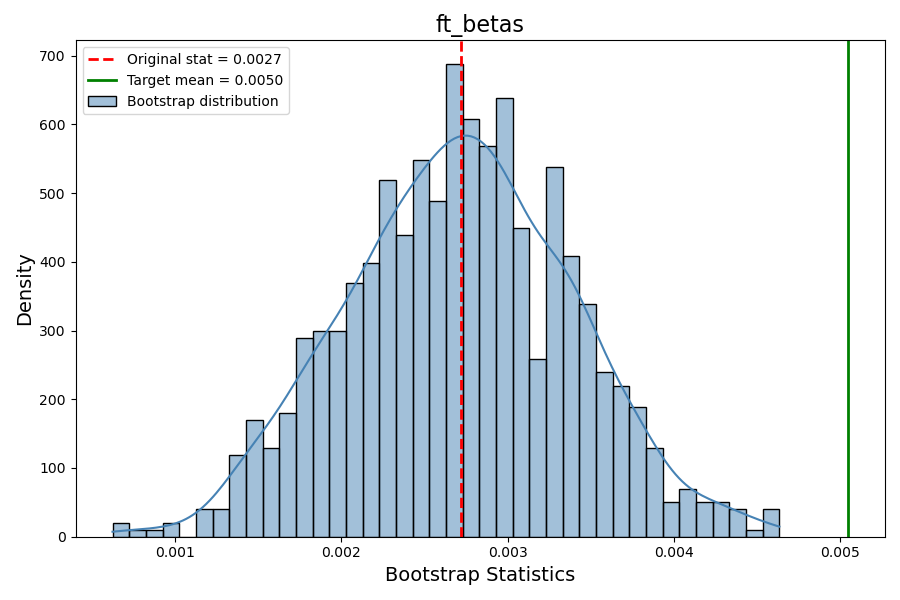
\includegraphics[width=\textwidth]{simulation_figure/ft_betas.png}
        \caption{Checkpoint-3: coefficient distribution}
    \end{subfigure}
    \hfill
    \begin{subfigure}[t]{0.48\textwidth}
        \centering
        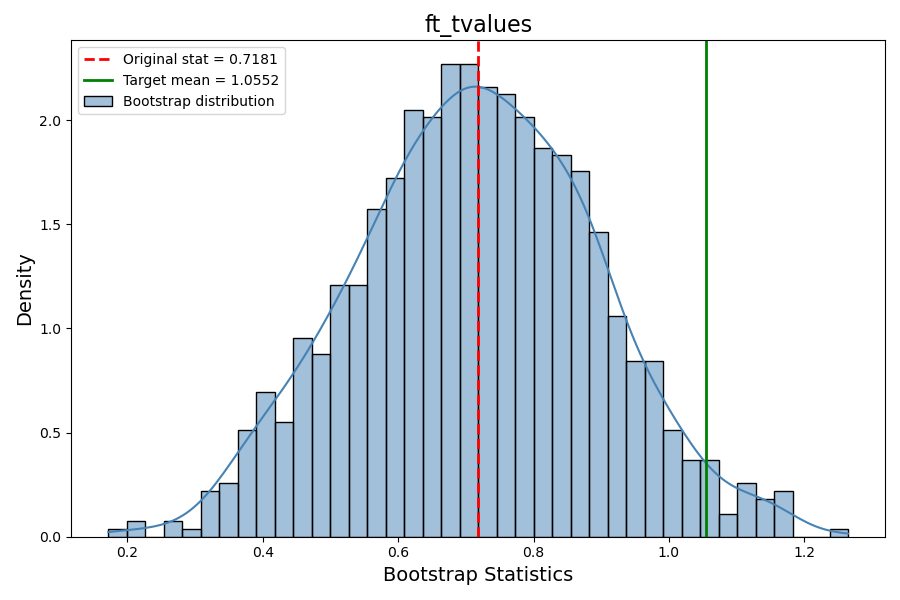
\includegraphics[width=\textwidth]{simulation_figure/ft_tvalues.png}
        \caption{Checkpoint-3: t-statistics distribution}
    \end{subfigure}
    \vspace{0.8em}

    %----------------- Base -----------------%
    \begin{subfigure}[t]{0.48\textwidth}
        \centering
        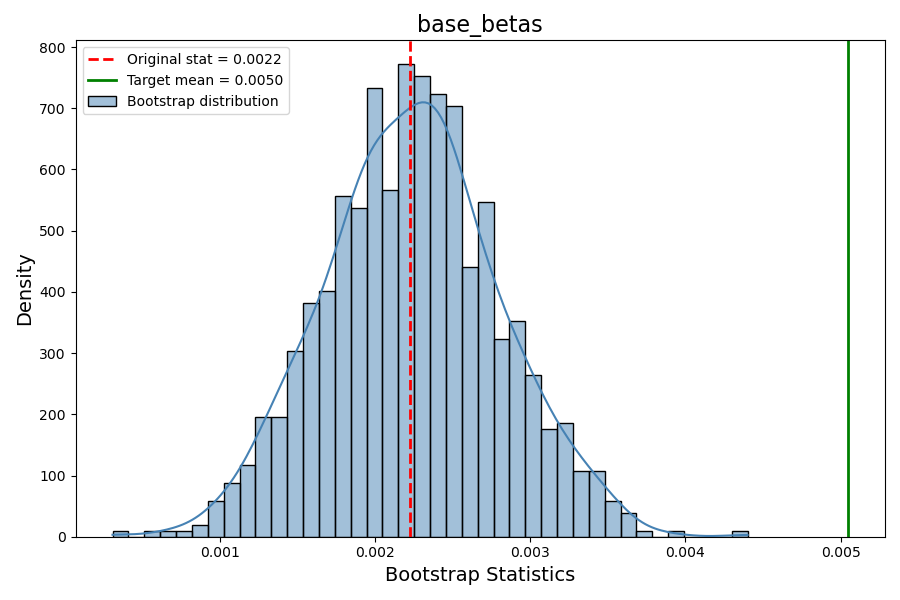
\includegraphics[width=\textwidth]{simulation_figure/base_betas.png}
        \caption{Backbone-0: coefficient distribution}
    \end{subfigure}
    \hfill
    \begin{subfigure}[t]{0.48\textwidth}
        \centering
        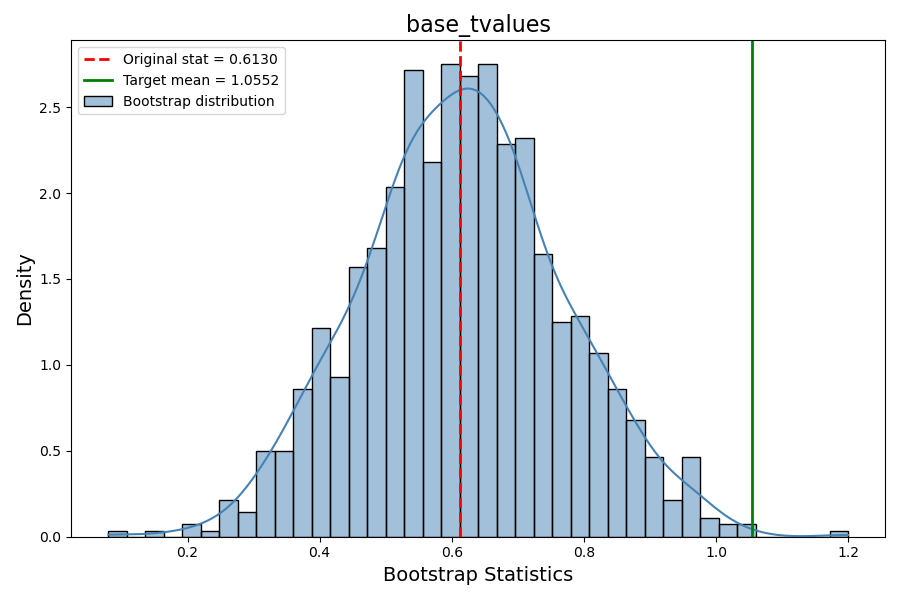
\includegraphics[width=\textwidth]{simulation_figure/base_tvalues.png}
        \caption{Backbone-0: t-statistics distribution}
    \end{subfigure}
    \caption{Bootstrap distributions of $Z_{t}^{M}$ coefficients and t-statistics for Checkpoint-3 and Backbone-0}
    \label{fig:ch2:bootstrap_ft_base}
\end{figure}

% coefficient
% base: 0.0022399151956866616, ft:0.0027096296763361653
% target: 0.005048811

% t-statistics
% base: 0.6168947613082458, ft: 0.7152094287360642
% target: -0.289101766
% 
% [CH2-092][Original Start]
% The bootstrap mean coefficient of $Z_{t}^{m}$ reached at 0.00271 for the Fine-tuned model and 0.00224 for the base model. Compared with the target coefficient (0.00505), there is a  20.97\% improvement. As for the t-statistics, there is a 15.94\% improvement from 0.61689 (base model) to 0.71521 (fine tuned model).
%
% The bootstrap mean coefficient of $Z_t^{m}$ is 0.00271 for the fine-tuned model and 0.00224 for the base model. Relative to the benchmark coefficient of 0.00505, the fine-tuned model reduces the estimation gap by 20.97\% compared with the base model. In terms of statistical significance, the corresponding $t$-statistic increases from 0.6169 for the base model to 0.7152 for the fine-tuned model, representing a 15.94\% improvement.
% [CH2-092][Original End]
% [CH2-130][Original Start]
% The bootstrap mean coefficient for $Z_t^m$ is 0.00271 for the fine-tuned model and 0.00224 for the baseline model. Relative to the benchmark coefficient (0.00505), the fine-tuned model reduces the estimation gap by 20.97\%. The corresponding $t$-statistic increases from 0.6169 to 0.7152, a 15.94\% improvement.
% [CH2-130][Original End]
The bootstrap mean coefficient for $Z_t^m$ is 0.00271 for Checkpoint-3 and 0.00224 for Backbone-0. Relative to the benchmark coefficient (0.00505), Checkpoint-3 reduces the estimation gap by 20.97\% versus the backbone comparison. However, the associated mean $t$-statistic only increases from 0.6169 to 0.7152, which remains far below conventional significance thresholds such as $|t|\approx1.96$. Accordingly, these regressions should be interpreted as exploratory directional evidence rather than as robust proof of market relevance.







% decision making accuracy 

\subsubsection*{Decision Prediction Performance}

% Finally, to assess factuality hallucination, we focus on the committee's voted actions. Specifically, we compare the model-generated policy decisions with the actual outcomes. To evaluate the effectiveness of our training in this stage, we compute the \textit{Decision-Making Accuracy} for both the \textit{Base Model} and the \textit{Fine-Tuned Model}.
% [Codex 修改版] 2026-02-26: 明确“决策预测”是下游评估任务，并避免与前文“Stage”命名混用。
% [CH2-131][Original Start]
% Finally, to assess factual grounding in a decision-relevant setting, we evaluate whether the model can infer the Committee’s voted action from the analytical context. Concretely, we compare model-predicted policy decisions with realized outcomes and report \textit{Decision-Making Accuracy} for a baseline model and a fine-tuned (Minutes-aligned) model.
%
% For this assessment, we use the non-decision sections from the FOMC Minutes as input prompts. Notably, because ``Committee Policy Action'' text was excluded from the analysis-generation dataset used for core training, the models are not directly trained on realized decisions. This design enables a more meaningful test of inferential capability: the models must predict the policy action based on the analytical discussion alone. We also use the supplementary Minutes (1994--2008) as an out-of-sample test set. Table~\ref{tab:ch2:decision_acc} reports the resulting decision-prediction accuracy.
%
% ... legacy accuracy tables and synthetic-Minutes table removed ...
% [CH2-131][Original End]
Finally, we evaluate decision-result exports for Backbone-0 and Checkpoint-4 on a common meeting-date-deduplicated set. To place the LLM results in context, we also compute historical baselines on the same meetings, and the Chapter 2 v2 pipeline additionally supports multinomial-logit and market-implied comparisons when the required data are available. Because model outputs sometimes fail to return a valid boxed vote, invalid predictions are reported separately and counted as errors in accuracy.

The deduplicated archive contains 237 meetings spanning March 23, 1993 to January 29, 2025. For comparability, we collapse detailed rate choices into three coarse classes: \textit{Cut}, \textit{No change}, and \textit{Raise}. Table~\ref{tab:ch2:decision_acc} reports overall accuracy, balanced accuracy, macro-F1, and invalid-vote counts. Table~\ref{tab:ch2:decision_confusion} reports the corresponding confusion matrices for the non-trivial predictors; these matrices count only valid three-class outputs, while invalid votes are excluded from the matrix and tracked separately.

% [Codex 修改版] 2026-04-17: 增加基于 archived decision-summary workbook 的 raw exact-match 补充说明，同时不在正文暴露目录拼写错误。
A complementary exact-match check on the archived decision-summary workbook uses all 241 decision rows before meeting-date deduplication and retains the original detailed vote labels (e.g., 25/50/75 basis-point moves). On this finer-grained criterion, Backbone-0 reaches 49.79\% exact match with 64 invalid detailed votes, while Checkpoint-4 reaches 58.92\% with 61 invalid detailed votes. These exact-match rates are not directly comparable to the three-class results in Table~\ref{tab:ch2:decision_acc}, but they show that the decision-specific branch improves relative to Backbone-0 on the archived workbook even though it still trails the simple lag-1 baseline once the evaluation is collapsed to policy direction.

\begin{table}[htbp]
    \centering
    \footnotesize
    \begin{tabular}{l c c c c}
        \toprule
        \textbf{Model} & \textbf{$n$ Meetings} & \textbf{Accuracy} & \textbf{Balanced Accuracy} & \textbf{Macro-F1} \\
        \midrule
        Backbone-0 & 237 & 0.5190 & 0.5434 & 0.5591 \\
        Checkpoint-4 & 237 & 0.6034 & 0.5550 & 0.5995 \\
        Majority baseline & 237 & 0.7089 & 0.3333 & 0.2765 \\
        Lag-1 action baseline & 237 & \textbf{0.7384} & \textbf{0.6424} & \textbf{0.6424} \\
        \midrule
        Backbone-0 invalid votes & \multicolumn{4}{c}{64} \\
        Checkpoint-4 invalid votes & \multicolumn{4}{c}{61} \\
        \bottomrule
    \end{tabular}
    \caption{Decision Prediction on Meeting-Date-Deduplicated Archived Outputs}
    \label{tab:ch2:decision_acc}
\end{table}

\begin{table}[htbp]
    \centering
    \scriptsize
    \begin{tabular}{l l c c c}
        \toprule
        \textbf{Model} & \textbf{Actual Class} & \textbf{Pred.\ Cut} & \textbf{Pred.\ No change} & \textbf{Pred.\ Raise} \\
        \midrule
        \multirow{3}{*}{Backbone-0}
            & Cut & 9 & 2 & 2 \\
            & No change & 3 & 79 & 43 \\
            & Raise & 0 & 0 & 35 \\
        \midrule
        \multirow{3}{*}{Checkpoint-4}
            & Cut & 8 & 2 & 4 \\
            & No change & 5 & 103 & 22 \\
            & Raise & 0 & 0 & 32 \\
        \midrule
        \multirow{3}{*}{Lag-1 action baseline}
            & Cut & 15 & 11 & 0 \\
            & No change & 11 & 137 & 20 \\
            & Raise & 0 & 20 & 23 \\
        \bottomrule
    \end{tabular}
    \caption{Decision Confusion Matrices for Valid Three-Class Outputs}
    \label{tab:ch2:decision_confusion}
\end{table}

Table~\ref{tab:ch2:decision_acc} shows that historical baselines remain strong. The majority baseline benefits from the dominance of ``No change'' meetings and therefore attains high raw accuracy, but its balanced accuracy and macro-F1 are weak. The lag-1 baseline performs best among the simple persistence rules reported here; multinomial-logit and market-implied baselines should be interpreted as additional context when their required inputs are available.

Relative to Backbone-0, the decision-specific branch now looks meaningfully better in the updated archived workbook: Checkpoint-4 reaches 0.6034 accuracy, 0.5550 balanced accuracy, and 0.5995 macro-F1, versus 0.5190, 0.5434, and 0.5591 for Backbone-0. It also reduces invalid votes from 64 to 61. However, this improvement is not enough to overturn the baseline comparison, because the lag-1 rule still dominates both LLM checkpoints on all three coarse metrics.

The confusion matrices clarify where the models succeed and fail. Backbone-0 overpredicts ``Raise'' for many ``No change'' meetings, while Checkpoint-4 reduces this particular error and materially improves the ``No change'' diagonal. At the same time, both LLM checkpoints still struggle on ``Cut'' relative to the lag-1 baseline, and invalid boxed votes remain non-trivial. Consequently, the archived evidence supports a narrower claim than the original draft: policy-direction inference is possible and Checkpoint-4 improves over Backbone-0 on the archived workbook, but the overall system is still weaker than a simple historical persistence rule on this dataset.

% [Codex 修改版] 2026-04-17: 集中写明当前 Chapter 2 的证据边界与未完成比较。
\subsection*{Limitations and Evidence Boundary}

The evidence in this chapter should be interpreted with several explicit limits in mind. First, the canonical split is meeting-level but random rather than chronological, so the reported textual and decision results should be read as held-out meeting validation rather than as forward-only time-series generalization. Second, the decision comparison is strongest when the same held-out meeting set is used for Backbone-0, Checkpoint-4, majority class, lag-1 persistence, multinomial logit, and any available market-implied baseline; if market data coverage is incomplete, the resulting comparison should be labeled accordingly. Third, the sentiment--return regression moves the coefficient estimate in the expected direction, but the associated $t$-statistics remain far below conventional significance thresholds. Finally, while optimizer, scheduler, reward, checkpoint lineage, and runtime configuration are now recorded in machine-readable manifests, the econometric evidence remains exploratory rather than definitive.









\section{Conclusion}\label{ch2:sec:conclusion}

% [CH2-096][Original Start]
% In conclusion, our research introduces a novel methodology for generating structured synthetic text data. More specifically, we have established that a fine-tuned Large Language Model (LLM) can effectively produce simulations of the Federal Open Market Committee (FOMC) Minutes. Empirical evidence demonstrates that the fine-tuned model outperforms the base model in generating responses that are similar to structured texts. Moreover, our findings indicate that the fine-tuned model possesses the capability to analyze data in a manner reflective of the FOMC's approach. This enables the model to rewrite the Minutes using simulated input data, offering fresh perspectives for risk management professionals concerning the impact of government announcements on the financial sector.
% [CH2-096][Original End]
% [CH2-132][Original Start]
% In conclusion, this chapter presents a framework for generating structured synthetic policy text with a fine-tuned LLM. The empirical results show that the Minutes-aligned model outperforms the baseline in textual fidelity, input grounding, and decision-relevant downstream tasks. These findings support the use of LLM-based policy-text simulation for macro-financial scenario analysis and risk-management research.
% [CH2-132][Original End]
In conclusion, this chapter presents a checkpointed framework for generating structured synthetic policy text with a post-trained LLM. The strongest empirical result is that Checkpoint-3 improves textual fidelity relative to Checkpoint-2 on the held-out Minutes split, while the leave-one-out masking tests show that generated sections remain sensitive to the conditioning indicators. On the decision task, Checkpoint-4 should be evaluated against Backbone-0 and the full baseline set on the same deduplicated held-out meetings. More broadly, the sentiment--return regressions and decision-prediction exercises remain exploratory because the split is random rather than temporal and the regression $t$-statistics stay well below conventional significance thresholds.

% Nonetheless, several avenues for future research remain open. Primarily, there is a need for the model to not only ensure consistency in its output but also sufficiency, ensuring that all pertinent economic and financial information from the prompts is included in the responses. To this end, employing the Shapley Value ($\mathcal{SV}$) to assess the marginal contribution of each prompt to the response could prove insightful. Given that the inclusion of additional prompts should ideally yield non-decreasing informational content, monitoring the Shapley Value could help in optimizing the model's responsiveness to new information.
% [Codex 修改版] 2026-02-26: 与本文采用的 leave-one-out 贡献度指标保持一致，并将“精确 Shapley”作为可扩展方向。
Nonetheless, several avenues for future research remain open. Primarily, beyond consistency, the model should also ensure \textit{sufficiency}: generated sections should incorporate the relevant economic and financial information contained in the prompts. In this chapter, we quantify grounding using a leave-one-out masking contribution score. Future work could extend this analysis toward more comprehensive Shapley-style attribution (e.g., subset sampling approximations), which would provide a stronger notion of expected marginal contribution when many prompts interact nonlinearly.

% [CH2-097][Original Start]
% Additionally, the use of standardized prompts presents an efficient pathway for generating results, eliminating the necessity for users to guide the model through multiple steps to achieve desired outcomes. Therefore, an upcoming focus will be to rigorously evaluate the generative capacity of such standardized prompts, ensuring they elicit responses that are both informative and contextually appropriate. Through these endeavors, we aim to refine our model further, enhancing its utility in the financial domain and beyond.
%
% By addressing these research gaps, we anticipate advancing the capabilities of our fine-tuned model, making it an even more powerful tool for simulating complex textual data, particularly in scenarios requiring nuanced understanding and detailed analysis, such as in financial risk assessment.
% [CH2-097][Original End]
Future work should further validate standardized prompt templates, improve robustness under distribution shifts, and extend attribution methods beyond leave-one-out masking. These directions can strengthen reliability and expand the practical value of synthetic policy communication in financial applications.
